\documentclass[12pt, a4paper]{article}
\usepackage{cmap}
\usepackage[T2A]{fontenc}
\usepackage[utf8]{inputenc}
\usepackage[english,russian]{babel}
\usepackage{amsmath,amsfonts,amssymb,amsthm,mathtools}
\usepackage[left=20mm, top=15mm, right=20mm, bottom=15mm, includehead, includefoot]{geometry}
\usepackage{multirow}
\usepackage{array}
\usepackage{multicol}
\usepackage{graphicx}
\usepackage{wrapfig}
\usepackage{indentfirst}
\usepackage{fancyhdr}
\usepackage{lipsum}
\usepackage{wallpaper}
\usepackage{fix-cm}
\usepackage{csquotes}
\usepackage{hyperref}

\hypersetup{
    colorlinks=false,
    linktoc=all
}

%=======================================SQ  CASES====================================
\makeatletter
\newenvironment{sqcases}{%
  \matrix@check\sqcases\env@sqcases
}{%
  \endarray\right.%
}
\def\env@sqcases{%
  \let\@ifnextchar\new@ifnextchar
  \left\lbrack
  \def\arraystretch{1.2}%
  \array{@{}l@{\quad}l@{}}%
}
\makeatother
%=======================================SQ  CASES====================================

\fancyhf{}
\renewcommand{\headrulewidth}{1pt}
\renewcommand{\footrulewidth}{1pt}
\chead{\leftmark}
\rfoot{\rightmark}
\lfoot{\thepage}

\graphicspath{{./visuals/}}
\setlength{\columnsep}{1cm}
\linespread{1}
\pagestyle{fancy}
\newcommand{\di}{\mathrm{d}}
\newcommand{\grad}{\mathrm{grad}}
\newcommand{\cov}{\mathrm{cov}}
\newcommand{\dop}{\textrm{доп.}}
\newcommand{\kr}{\textrm{кр.}}
\newcommand{\const}{\textit{const}}
\newcommand{\irv}[1]{\langle #1 \rangle}
\newcommand{\defeq}{\stackrel{\mathclap{\mathrm{def}}}{=}}
\newcommand{\eu}{\textrm{e}}
\author{ГМВ}
\title{Вышмат}

\begin{document}

\thispagestyle{empty}

\ThisCenterWallPaper{1}{forsatz.pdf}

\vspace*{63mm}
\begin{center}
{\fontsize{80}{90}\selectfont \textbf{\textsc{Высшая \\ Математика}}} \\

\vspace{5mm}

{\Large Лекции,} \\

\vspace{5mm}

записанные студентом М. В. Григорьевым \\ после прослушанного курса Н. А. Волковой

\vspace{5mm}

СПбГУ \\
2020
\end{center}
\vspace*{\fill}

\newpage\clearpage\pagenumbering{arabic}

\tableofcontents

\newpage

\section{Методы математической статистики}

\textbf{Математическая статистика} - о математической обработке результатов измерений, которые касаются большого количества явлений (слишком большого, чтобы рассмотреть это всё).

В статистике вместо понятия \textit{случайная величина} часто используют понятие \textit{признак}.

(\textit{вставить материал из прописанных билетов: "введение в статистику"})

\subsection{Введение}

\textbf{Математическая статистика} - методы обработки эмпирических исследований.

\subsubsection{Основные задачи математической статистики}
\begin{itemize}
 \item определение закона распределения изучаемой \textit{величины} (признака, вариации);
 \item определение \textit{параметров} распределения - построение оценок и интервалов изменения параметра;
 \item построение \textit{критериев} для оценки вероятностей сделать правильный выбор закона распределения.
\end{itemize}

\subsubsection{Основные понятия}
\textbf{Случайная выборка} - случайный вектор $(x_1, x_2, \cdots, x_n) \in \mathbb{R}^n$, где $x_i, \quad i = \overline{1, n}$ - случайные величины с одинаковым законом распределения.

\textbf{Оценкой} неизвестного параметра распределения $\theta$ называется функция
\[\hat{\theta}_n = \hat{\theta}_n(x_1, x_2, \cdots, x_n) \]

Оценка $\hat{\theta}_n$ \textbf{несмещённая}, если
\[M(\hat{\theta}_n) = \theta \]

Оценка $\hat{\theta}_n$ \textbf{состоятельная}, если она сходится по вероятности к $\theta$, то есть:
\[P(|\hat{\theta}_n - \theta| < \varepsilon) \xrightarrow[n \to +\infty]{} 1 \]

\textbf{Пример} Закон Больших Чисел в форме Бернулли:
\[P(| \frac{m}{n} - p| < \varepsilon) \xrightarrow[n \to +\infty]{} 1 \]
То есть относительная частота $\frac{m}{n}$ - состоятельная оценка для теоретической вероятности $p$.

Оценка называется \textbf{эффективной}, если $D(\hat{\theta}_n(x_1, x_2, \cdots, x_n)) = D_{\min}$ (минимальная дисперсия из всех дисперсий оценок данного параметра).

Следовательно, надо стараться, чтобы оценка параметра $\theta$ была \textit{несмещённой}, \textit{состоятельной}, \textit{эффективной}.

Кроме точечных оценок существуют интервальные оценки. \textbf{Доверительный интервал} - оценка неизвестного параметра $\theta$ снизу и сверху, то есть интервал
\[(\underline{\theta}_n(x_1, x_2, \cdots, x_n), \overline{\theta}_n(x_1, x_2, \cdots, x_n)) \]
такой что $\underline{\theta}_n < \theta < \overline{\theta}_n$ с вероятностью $(1-2\alpha)$, которая называется доверительной вероятностью, $\alpha$ - уровень значимости (несколько процентов на практике), то есть:
\[P(\theta \in (\underline{\theta}_n, \overline{\theta}_n)) = 1-2\alpha \]

\textbf{Замечание}: на практике используют $1-2\alpha = 0.95, 0.99, 0.999, \cdots$

\subsubsection{Свойства выборочного среднего и выборочной дисперсии}
\begin{center}
\begin{Large}
Выборочное среднее
\end{Large}
\end{center}

\[\overline{X} = \frac{1}{n} \sum_{k=1}^n x_k \]

Утверждение 1: $\overline{X}$ - несмещённая оценка.

Доказательство: $X$ - случайная величина с $MX = a$, а $x_1, x_2, \cdots, x_n$ - его реализации, то есть $x_i, \quad i = \overline{1, n}$ - случайные независимые величины с тем же законом распределения.

Тогда из свойств матожидания имеем:
\[M(\overline{X}) = M(\frac{1}{n} \sum_{i=1}^n x_i) = \{\textrm{по свойствам матожидания} \} = \frac{1}{n} M(\sum_{i=1}^n x_i) = \frac{1}{n} \sum_{i=1}^n M(x_i) = \]
\[= \frac{1}{n} \sum_{i=1}^n a = \frac{n \cdot a}{n} = a \]

Утверждение 2: $\overline{X}$ - состоятельная оценка.

Доказательство:
\[P(| \frac{1}{n} \sum_{i=1}^n x_i - a| < \varepsilon) \xrightarrow[n \to +\infty]{} 1\]
по следствию ЗБЧ в форме Чебышёва.

Утверждение 3: $D(\overline{X}) = \frac{DX}{n}$.

Доказательство:
\[D(\overline{X}) = D(\frac{1}{n} \sum_{i=1}^n x_i) = \frac{1}{n^2} D(\sum_{i=1}^n x_i) = \{в силу независимости x_i \} = \frac{1}{n^2} \sum_{i=1}^n DX = \frac{n \cdot DX}{n^2} = \frac{DX}{n} \]

Следствие: $D(\overline{X}) \xrightarrow[n \to +\infty]{} 0$.

То есть выборочное среднее - несмещённая, эффективная и состоятельная оценка матожидания.

\begin{center}
\begin{Large}
Выборочная дисперсия
\end{Large}
\end{center}

\[S^2 = \frac{1}{n} \sum_{k=1}^n (x_k - \overline{X})^2 \]

Утверждение 1: $S^2$ - смещённая оценка.

Доказательство:
\[M(S^2) = M(\frac{1}{n} \sum_{k=1}^n (x_k - \overline{X})^2) = M(\frac{1}{n} \sum_{k=1}^n (x_k - \frac{1}{n} \sum_{i=1}^n x_i)^2) = \{DX = MX^2 - (MX)^2 \} = \]
\[= \frac{1}{n} M(\sum_{k=1}^n x_k^2) - \frac{1}{n^2} \sum_{k=1}^n M(x_k^2) - \frac{2}{n^2} \sum_{i,k=1}^n M(x_i \cdot x_k) = \]
\[= \{\textrm{не умаляя общности MX=0} \Rightarrow M(X^2) = M(X^2) - (MX)^2 (=0) = DX \} = \]
\[= \frac{n-1}{n^2} \sum_{i=1}^n DX = \frac{n-1}{n^2} DX \xrightarrow[n \to +\infty]{} DX \]

Отсюда следует, что несмещённой оценкой для дисперсии будет:
\[S_1^2 = \frac{n}{n-1} S^2 = \frac{1}{n-1} \sum_{i=1}^n (x_i - \overline{X})^2 \]
\textbf{несмещённая выборочная дисперсия}.

Можно показать, что несмещённая выборочная дисперсия состоятельная и эффективная.

\textbf{Замечание:} состоятельная и несмещённая оценка дисперсии - выборочная несмещённая дисперсия $S_1^2 = \frac{1}{n-1} \sum_{i=1}^n (x_i - \overline{x})^2$, а несмещённой, состоятельной и \textit{эффективной} будет:
\[S^2_{*} = \frac{1}{n} \sum_{i=1}^n (x_i - MX)^2 \]
Для этого должно быть известным $MX$.

\subsubsection{Метод наибольшего правдоподобия для оценок параметров распределения}

\begin{center}
\begin{Large}
Дискретная величина
\end{Large}
\end{center}

Пусть $X$ - \textbf{дискретная} случайная величина и ряд распределения: $P(X=x_i) = P(x_i, \theta)$ - содержит неизвестный параметр $\theta$.

\textbf{Функцией правдоподобия} для выборки $(x_1, x_2, \cdots, x_n)$ называется функция вида:
\[L(x_1, x_2, \cdots, x_n) = P(x_1, \theta) \cdot P(x_2, \theta) \cdots P(x_n, \theta) \]
В качестве оценки параметра берут $\theta^*$, при котором $L(x_1, x_2, \cdots, x_n, \theta^*) = \max L$.

Проще дифференцировать сумму, чем произведение. Вместо $L$ рассмотрим $\ln L$, которая принимает экстремальные значения в тех же точках, что и $L$ (ввиду монотонного возрастания логарифма). Тогда условие экстремума:
\[\frac{\partial \ln L}{\partial \theta} = 0 \]
или
\[\frac{\partial}{\partial \theta} [\ln \prod_{i=1}^n P(x_i, \theta)] = \frac{\partial}{\partial \theta} \sum_{i=1}^n \ln (P(x_i, \theta)) = \sum_{i=1}^n \frac{\frac{\partial P(x_i, \theta)}{\partial \theta}}{P(x_i, \theta)} = 0 \]

\textbf{Замечание:} в общем случае, когда закон распределения содержит несколько неизвестных параметров $\theta_1, \theta_2, \cdots, \theta_k$, функция правдоподобия тоже будет содержать $k$ неизвестных аргументов $L(x_1, \cdots, x_n, \theta_1, \cdots, \theta_k)$, и тогда максимально правдоподобной оценкой будет решение системы из $k$ уравнений, а именно:
\[\frac{\partial}{\partial \theta_j} (\ln L(x_1, \cdots, x_n, \theta_1, \cdots, \theta_k)) = 0, \quad j=\overline{1, k} \]

\begin{center}
\begin{Large}
Непрерывная величина
\end{Large}
\end{center}

Пусть $X$ - \textbf{непрерывная} случайная величина с неизвестным параметром распределения $\theta$,  но известным видом функции плотности распределения вероятностей $f(x, \theta)$, тогда по аналогии с дискретным случаем по заданной выборке $(x_1, x_2, \cdots, x_n)$ строим \textbf{функцию правдоподобия} $L(x_1, \cdots, x_n, \theta) = \prod_{i=1}^n f(x_i, \theta)$ и ищем $\theta^*$, такое что $L(x_1, \cdots, x_n, \theta^*) = \max L$.

Вместо самой функции $L$ рассматриваем её логарифм, как и в прошлом случае. Решаем уравнение:
\[\frac{\partial}{\partial \theta} \ln L(x_1, \cdots, x_n, \theta) = 0 \]

\textbf{Замечание:} если $f(x_1, \cdots, x_n, \theta_1, \cdots, \theta_k)$ - функция с $k$ параметрами, то оценкой $\theta_1, \cdots, \theta_k$ будет решение системы уравнений:
\[\frac{\partial}{\partial \theta_j} (\ln L(x_1, \cdots, x_n, \theta_1, \cdots, \theta_k)) = 0, \quad j=\overline{1, k} \]

\textit{Оценка, полученные методом максимального правдоподобия:
\begin{itemize}
 \item не обязана быть состоятельными;
 \item может быть смещённой;
 \item может быть не единственной.
\end{itemize}}

\textbf{Пример:} $X$ - случайная величина с дискретным пуассоновским распределением:
\[P(X=m) = \frac{\exp [-\lambda] \cdot \lambda^m}{m!} \]
с неизвестным параметром $\lambda$. Пусть $(x_1, \cdots, x_n), \quad x_i \in \mathbb{N}, \quad i = \overline{1, n}$.

Функция правдоподобия:
\[L(x_1, \cdots, x_n, \lambda) = \prod_{i=1}^n \frac{\exp [-\lambda] \lambda^{x_i}}{x_i!} \]

Логарифм функции:
\[\ln L(x_1, \cdots, x_n, \lambda) = \ln \prod_{i=1}^n \frac{\exp [-\lambda] \lambda^{x_i}}{x_i!} = \sum_{i=1}^n \ln \frac{\exp [-\lambda] \lambda^{x_i}}{x_i!} \]

Условие экстремума:
\[\frac{\partial}{\partial \lambda} \sum_{i=1}^n \ln \frac{\exp [-\lambda] \lambda^{x_i}}{x_i!} = 0 \quad \Leftrightarrow \quad \sum_{i=1}^n (-\lambda - x_i \ln \lambda - 0) = 0 \]
\[\mathfrak{Differenzierung} \]
\[\lambda = \frac{\sum_{i=1}^n x_i}{n} = \overline{X} \]

\subsubsection{Метод моментов для оценивания параметров распределения}
Пусть $F(x, \theta_1, \theta_2, \cdots, \theta_k)$ - функция распределения с $k$ неизвестными параметрами, но известного вида. Соответственно моменты (начальные $\nu_i$ и центральные $\mu_i$) будут функциями параметров $\theta_1, \cdots, \theta_k$. По выборке определяют выборочные (начальные $\alpha_i$ или центральные $\beta_i$) моменты и приравнивают теоретически вычисленные к выборочным:
\[\nu_i(\theta_1, \cdots, \theta_k) = \alpha_i, \quad i = \overline{1, k} \]
\[\mu_i(\theta_1, \cdots, \theta_k) = \beta_i, \quad i = \overline{1, k} \]

\textbf{Замечание:} надёжность метода моментов растёт с объёмом выборки.

\textbf{Пример:} пусть $X$ - случайная величина с равномерным распределением:
\begin{wrapfigure}{r}{0.3\textwidth}
  \centering
  \vspace{5mm}
  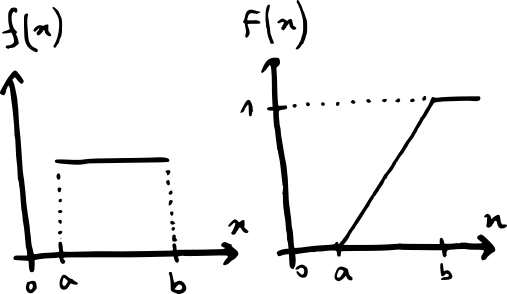
\includegraphics[width=0.3\textwidth]{01}
  \vspace{-4mm}
  \caption{Плотность и функция равномерного распределения}
\end{wrapfigure}
\[\begin{cases} 0, & x \leq a \\
\frac{x-a}{b-a}, & a \leq x \leq b \\
1, & x > b \\
\end{cases} \]
Имеем 2 параметра: $a, b$. Известны теоретические моменты:
\[\nu_1 = MX = \frac{b+a}{2} \hspace{3cm} \mu_2 = DX = \frac{(b-a)^2}{12} \]
Находим $\overline{X}$ и $S^2_1$ и составим систему уравнений:
\[\begin{cases} \frac{b^* + a^*}{2} = \overline{X} \\
\frac{(b^* - a^*)^2}{12} = S^2_1 \\
\end{cases} \quad \Leftrightarrow \quad
\begin{cases} a^* = \overline{X} - \sqrt{3S_1^2} \\
b^* = \overline{X} + \sqrt{3S_1^2} \\
\end{cases} \]

Так как $\overline{X}$ и $S^2_1$ - несмещённые величины, то и их оценки будут несмещёнными.

\subsection{Интервальные оценки}
\subsubsection{Доверительные интервалы и доверительная вероятность}
Основная проблема - построить доверительный интервал $[\theta_1, \theta_2]$, куда входит величина с доверительной вероятностью $1-2\alpha$, на практике $0.9$, $0.95$, $0.99$, $0.999$.

\subsubsection{Построение доверительных интервалов для нормально распределённых случайных величин}

\begin{center}
\begin{Large}
Дисперсия $\sigma^2$ известна
\end{Large}
\end{center}

$X$ - случайная величина (признак) генеральной совокупности, такой что: $X \in N(a, \sigma^2)$, где $\sigma$ - точность измерительной системы - известна. Имеем выборку $x_1, x_2, \cdots, x_n$. Тогда в качестве точечной оценки для $a$ берётся несмещённая, состоятельная, эффективная оценка - \textit{выборочное среднее} $\overline{X} = \frac{1}{n} \sum_{i=1}^n x_i$. Тогда дисперсия случайной величины $\overline{X} = \frac{1}{n} \sum_{i=1}^n x_i, \quad x_i \in N(a, \sigma^2)$ есть $M\overline{X} = a, \quad D\overline{X} = \frac{DX}{n} = \frac{\sigma^2}{n}$, то есть $\overline{X} = N(a, \frac{\sigma^2}{n})$, тогда $\frac{\overline{X} - a}{\sigma^2 / \sqrt{n}} \in N(0, 1)$.

\begin{wrapfigure}[8]{l}{0.3\textwidth}
  \centering
  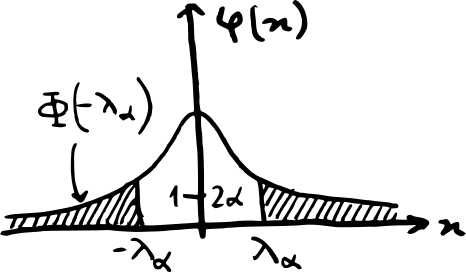
\includegraphics[width=0.3\textwidth]{02}
  \vspace{-4mm}
  \caption{Плотность стандартного нормального распределения}
\end{wrapfigure}

Следовательно, $P(|\frac{\overline{X} - a}{\sigma / \sqrt{n}}| < \lambda_{\alpha}) = 1 - 2\alpha$, где $\beta = 1-2\alpha$ - доверительная вероятность (0.9, 0.95, 0.99, 0.999), а $2\alpha$ - уровень значимости.

\textbf{Замечание} к иллюстрации: если $\Phi (x) = \int \limits_{-\infty}^x \frac{1}{\sqrt{2\pi} \exp [-\frac{t^2}{2}]} \di t$ - функция стандартного нормального распределения, то $\alpha = \Phi(\lambda_{\alpha})$, то есть $\lambda_{\alpha}$ - корень этого трансцендентного уравнения, который можно взять в соответствующих таблицах.

\begin{center}
\begin{tabular}{|c|c|c|c|c|}
\hline
$\beta$ & 0.9 & 0.95 & 0.99 & 0.999 \\
\hline
$\alpha$ & 0.05 & 0.025 & 0.005 & 0.0005 \\
\hline
$\lambda_{\alpha}$ & 1.64 & 1.96 & 2.51 & 3.3 \\
\hline
\end{tabular}
\end{center}

Тогда с вероятностью (надёжностью) $\beta = 1-2\alpha$ доверительный интервал:
\[|\frac{\overline{X} - a}{\sigma / \sqrt{n}}| < \lambda_{\alpha} \quad \Leftrightarrow \]
\[\Leftrightarrow \quad \overline{X} - \lambda_{\alpha} \frac{\sigma}{\sqrt{n}} < a < \overline{X} + \lambda_{\alpha} \frac{\sigma}{\sqrt{n}} \quad \Leftrightarrow \]
\[\Leftrightarrow \quad a \in (\overline{X} - \lambda_{\alpha} \frac{\sigma}{\sqrt{n}}, \overline{X} + \lambda_{\alpha} \frac{\sigma}{\sqrt{n}}) \textrm{покрывает параметр} a \]

\begin{center}
\begin{Large}
Дисперсия $\sigma^2$ неизвестна
\end{Large}
\end{center}

Пусть признак $X \in N(a, \sigma^2)$, где $a$, $\sigma$ - неизвестны. По выборке $(x_1, x_2, \cdots, x_n)$ определим точечные оценки $a$ и $\sigma^2$ - выборочное среднее $\overline{X} = \frac{1}{n} \sum_{i=1}^n x_i$ и несмещённая выборочная дисперсия:
\[S_1^2 = \frac{1}{n-1} \sum_{i=1}^n (x_i - \overline{X})^2 = \frac{1}{n-1} (\sum_{i=1}^n x_i^2 - \overline{X})^2 \]
($\frac{n}{n-1}$ - поправка Бесселя). 

Случайная величина $(\tau_n, t_n, T)$, равная $\frac{\overline{X} - a}{S_1 / \sqrt{n}}$ - распределение Стьюдента с $n-1$ степенями свободы, плотность распределения которого имеет вид:
\[S_{n-1}(t) = \frac{\Gamma (\tfrac{n}{2})}{\sqrt{\pi (n-1)} \Gamma (\tfrac{n-1}{2})} (1+\frac{t^2}{n-1})^{-\tfrac{n}{2}} \]
где $\Gamma (x) = \int \limits_0^{+\infty} \tau^{x-1} \mathrm{e}^{-\tau} \di \tau$. $S_{n-1}(t) = -S_{n-1}(-t)$, то есть функция чётная. Аналогично сказанному в пункте выше:
\[P(|\frac{\overline{X} - a}{S_1 / \sqrt{n}}| < t_{\alpha}) = 1-2\alpha = 1-2S_{n-1}(-t_{\alpha}) \]

\begin{wrapfigure}[11]{l}{0.28\textwidth}
  \centering
  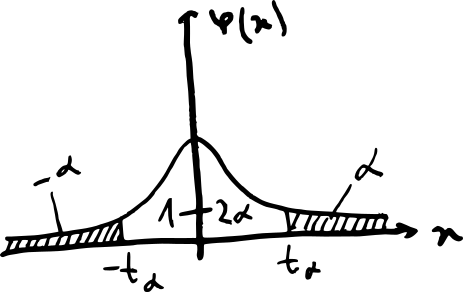
\includegraphics[width=0.28\textwidth]{03}
  \vspace{-4mm}
  \caption{Плотность стандартного нормального распределения}
\end{wrapfigure}

Корни уравнения $S_{n-1}(t_{\alpha}) = \alpha$ протабулированы. Отсюда можем получить соответствующую оценку для $a$ с надёжностью $1-2\alpha$, то есть доверительный интервал:
\[(\overline{X} - t_{\alpha} \frac{S_1}{\sqrt{n}}, \overline{X} + t_{\alpha} \frac{S_1}{\sqrt{n}}) \]

\textbf{Замечание:} оценка дисперсии $\sigma^2$ более сложна, так как соответствующая величина имеет отношение к более сложному распределению величины $\chi^2$.

\subsection{Исследование зависимостей между парами случайных признаков}

\subsubsection{Выборочные характеристики двумерного признака, характеризующие генеральную совокупность}

Имеем выборку $n$ упорядоченных пар значений двумерной случайной величины $(X, Y)$ - $((x_1, y_1), \cdots, (x_n, y_n))$.

Тогда \textbf{выборочными средними} для $X$, $Y$ называются характеристики вида:
\[\overline{X} = \frac{1}{n} \sum_{i=1}^n x_i \hspace{2cm} \overline{Y} = \frac{1}{n} \sum_{i=1}^n y_i \]

\textbf{Выборочной ковариацией} называется: 
\[R(X, Y) = r(X, Y) = \overline{\cov} (X, Y) = \frac{1}{n} \sum_{i=1}^n (x_i - \overline{X})(y_i - \overline{Y}) = \frac{1}{n} x_iy_i - \overline{XY} \]

\textbf{Выборочной дисперсией} называется величина:
\[S^2(X) = \frac{1}{n} \sum_{i=1}^n (x_i - \overline{X})^2 = \frac{1}{n} \sum_{i=1}^n x_i^2 - \overline{X}^2 \]
\[S^2(Y) = \frac{1}{n} \sum_{i=1}^n (y_i - \overline{Y})^2 = \frac{1}{n} \sum_{i=1}^n y_i^2 - \overline{Y}^2 \]

\textbf{Выборочным коэффициентом корреляции} называется величина:
\[k(X, Y) = \frac{r(X, Y)}{S(X)S(Y)} \]

\textbf{Утверждение}: при линейной зависимости $Y = aX + b$:
\[|k(X, Y)| = 1 \]
Принято говорить, что чем ближе коэффициент корреляции по модулю к 1, тем теснее связь между $X$ и $Y$.

\subsubsection{Линии регрессии}

\textbf{Линии регрессии} - моделирование линейной зависимости между $X$ и $Y$ вида $y = k_1x + b_1$ или $x = k_2y + b_2$. Тогда вводят следующие определения.

\begin{wrapfigure}{r}{0.25\textwidth}
  \centering
  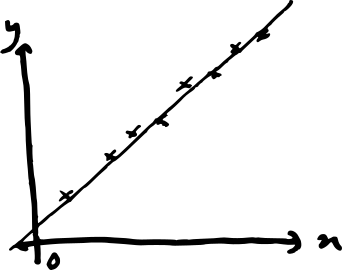
\includegraphics[width=0.25\textwidth]{04}
  \vspace{-7mm}
  \caption{Линия регрессии}
\end{wrapfigure}

\textbf{Выборочный коэффициент регрессии} $y$ на $x$ - величина, равная $l_0 = r(x, y) \frac{S(y)}{S(x)} = \frac{k(X, Y)}{S(X)}$. ВКР $x$ на $y$: $l_1 = \frac{k(X, Y)}{S(Y)}$.

Тогда уравнения регрессии примут вид:
\[y = \overline{y} + l_0(x-\overline{x}) \quad y \quad \textrm{на} \quad x \]
\[x = \overline{x} + l_1(y-\overline{y}) \quad x \quad \textrm{на} \quad y \]

\subsubsection{Метод наименьших квадратов (МНК)}

Эффективный метод, дающий при достаточно общих условиях состоятельную оценку параметров функциональной зависимости 2-х случайных величин. Чаще всего применяется для определения параметров линейной зависимости между случайными величинами $X$ и $Y$. В общем случае, постановка задачи выглядит следующим образом.

Даны $n$ наблюдений 2-х случайных величин $X$ и $Y$: $(x_1, y_1), \cdots, (x_n, y_n)$. Предполагается функциональная зависимость, зависящая от $k$ параметров $a_i, \quad i = \overline{1,k}$ вида $Y = f(X, a_1, a_2, \cdots, a_k)$, где вид $f$ считается известным.

\textbf{Примеры:}
\begin{figure}[h]
 \centering
 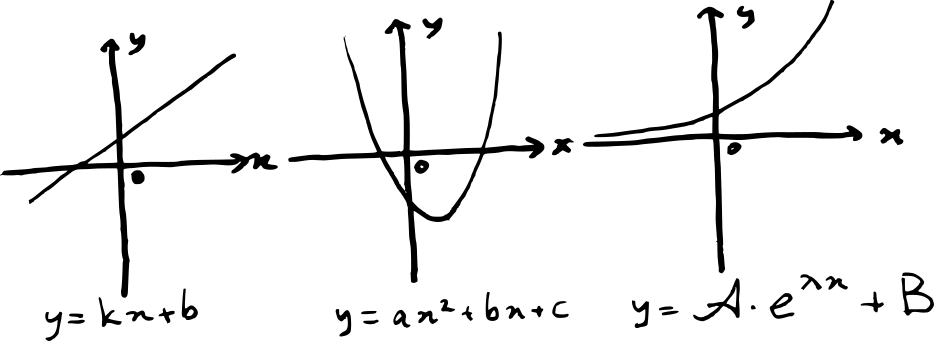
\includegraphics[width=0.6\textwidth]{05}
 \vspace{-4mm}
  \caption{Функциональные зависимости}
\end{figure}

Тогда в качестве значений неизвестных параметров принимаются те, что дают суммарное наименьшее отклонение от наблюдаемых значений $X$ и $Y$. Рассмотрим функцию:
\[Q(a_1, a_2, \cdots, a_k) = \sum_{i=1}^n (y_i - f(x_i, a_1, \cdots, a_k))^2 \xrightarrow[a_i]{} \min \]
Точки экстремума - это точки $(a_1^*, \cdots, a_k^*)$ - решения системы уравнений:
\[\frac{\partial Q}{\partial a_j} = 0, \quad j=\overline{1,k} \]

\textbf{Пример:} Определение параметров линейной зависимости $Y = kX + b$. Тогда:
\[Q(k, b) = \sum_{i=1}^n (y_i - kx_i - b)^2 \xrightarrow[a_i]{} \min \]
Значения $k^*$ и $b^*$ - решения системы уравнений:
\[\begin{cases}
\frac{\partial Q}{\partial k} = \sum_{i=1}^n 2(y_i - kx_i - b)(-x_i) = 0 \\
\frac{\partial Q}{\partial b} = \sum_{i=1}^n 2(y_i - kx_i - b)(-1) = 0 \\
\end{cases} \]

\subsection{Проверка статистических гипотез}

\subsubsection{Постановка задач}

\textbf{Статистической гипотезой} называют любое утверждение о законе распределения признака $X$ генеральной совокупности и его характеристиах (параметрах).

\textit{Самые важные}:
\begin{enumerate}
 \item Оценка параметра $\theta$ типа принадлежности к интервалу, сравнения с числом или определения значения.
 \item Данный признак $X$ имеет закон распределения $F_X(x, \theta_1, \cdots, \theta_k)$.
\end{enumerate}

Формулируются 2 \textit{альтернативные} (как правило) гипотезы $H_0$ и $H_1$, которая состоит в том, что не имеет места $H_0$.

\textbf{Статистический критерий} - это правило, которое по данной выборке $(x_1, x_2, \cdots, x_n)$ позволяет либо принять, либо отвергнуть гипотезу $H_0$.

Общая формулировка статистического критерия.
\begin{figure}[h]
 \centering
 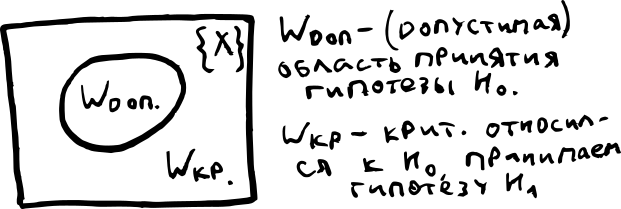
\includegraphics[width=0.5\textwidth]{06}
 \vspace{-4mm}
  \caption{Допустимая и критическая области}
\end{figure}

Статистическим критерием называется область $W_{\dop} \subset \mathbb{R}^n$, если $(x_1, \cdots, x_n) \in W_{\dop} \Rightarrow H_0$, если $(x_1, \cdots, x_n) \notin W_{\dop} \land (x_1, \cdots, x_n) \in W_{\kr} \Rightarrow$ гипотеза $H_0$ отвергается, и имеет место $H_1$.

\begin{center}
\begin{tabular}{|c|c|c|}
\hline
Гипотеза $H_0$ & Верна & Неверна \\
\hline
Принята & Правильно & Ошибка 2-го рода \\
Отвергнута & Ошибка 1-го рода & Правильно \\
\hline
\end{tabular}
\end{center}

Вероятность $\alpha$ - вероятность ошибки 1-го рода - \textit{уровень значимости}, который на практике принимает значения 0.05, 0.01, 0.005, 0.001.

Вероятность $\beta$ - сделать ошибку 2-го рода называется \textbf{оперативной характеристикой критерия}, а $\beta' = 1-\beta$ - называется \textbf{мощностью критерия}.

\textbf{Замечание:} на практике более существенна ошибка 2-го рода - принять партию бракованных изделий часто опаснее, чем забраковать партию хорошего.

\textbf{Пример} с оценкой параметра распределения с односторонним и двусторонним критерием. Пусть $\tilde{\theta}$ - выборочная оценка параметра $\theta$ - имеет плотность распределения $p(\tilde{\theta})$. Гипотеза $H_0: \quad \theta = \theta_0$. Если $\theta = \theta_0$ верно, то $M(\tilde{\theta}) = \theta_0$.

\begin{wrapfigure}[0]{r}{0.25\textwidth}
  \centering
  \vspace{-8mm}  
  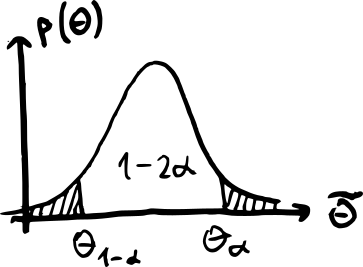
\includegraphics[width=0.25\textwidth]{07}
  \vspace{-9mm}
  \caption{Плотность распределения}
\end{wrapfigure}
\[P(\tilde{\theta} < \theta_{1-\alpha}) = \int \limits_{-\infty}^{\theta_{1-\alpha}} p(t) \di t = \alpha \]
\[P(\tilde{\theta} > \theta_{\alpha}) = \int \limits_{\theta_{\alpha}}^{+\infty} p(t) \di t = \alpha \]
\textit{Статистический критерий}: если выборочная оценка $\tilde{\theta} (x_1, \cdots, x_n) \in (\theta_{1-\alpha}, \theta_{\alpha})$, то гипотеза $\theta = \theta_0$ верна, в противном случае - нет. Предположим, что гипотеза $H_0$ - неверна и $\theta = \theta_0 \pm \alpha$.

\begin{figure}[h]
 \centering
 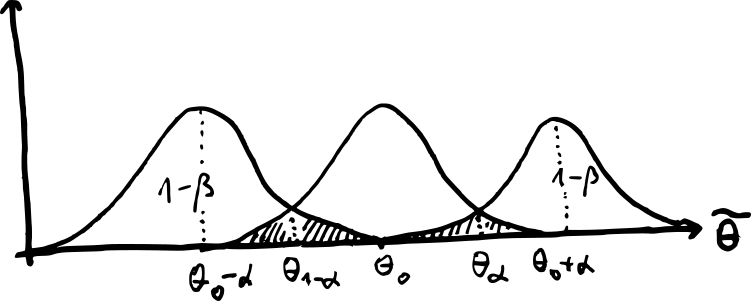
\includegraphics[width=0.5\textwidth]{08}
 \vspace{-4mm}
 \caption{Вероятности ошибок 1-го и 2-го рода}
\end{figure}

Тогда при фиксированном объёме выборки и при уменьшении веротяности ошибки 1-го рода вероятность ошибки 2-го рода возрастает. Чтобы уменьшить вероятности и $\alpha$, и $\beta$, нужно увеличить объём выборки.

\subsubsection{Проверка статистических гипотез о характере распределения}

\textbf{Критерий согласия Пирсона "хи-квадрат" ($\chi^2$)}. Гипотеза $H_0$: случайная величина $X$ имеет закон распределения $F_0(x)$. $H_1$ - не имеет этого закона распределения.

\textit{Статистический критерий}:
\[\chi^2 = \sum_{i=1}^l \frac{(m_i-np_i)^2}{np_i} = \sum_{i=1}^l \frac{m_i^2}{np_i^2} - n \]
где $m_i$ - число элементов в $i$-том интервале, $p_i$ - теоретически вычисленная вероятность $P(X \in \Delta i)$.

Результат наблюдений и вычислений:
\begin{center}
\begin{tabular}{|c|cccc|}
\hline
Интервал $\Delta_i$ & $\Delta_1$ & $\Delta_2$ & $\cdots$ & $\Delta_l$ \\
\hline
Эмп. частота $m_i$ & $m_1$ & $m_2$ & $\cdots$ & $m_l$ \\
\hline
Теор. частота $np_i$ & $np_1$ & $np_2$ & $\cdots$ & $np_l$ \\
\hline
\end{tabular}
\end{center}

По теореме Пирсона:
\[\chi^2 \xrightarrow[n \to +\infty]{} \chi^2_{l-1} \]
где $\chi^2 = \sum_{i=1}^n \chi^2_i$, а $\chi_i \in N(0, 1)$.

Тогда гипотеза $H_0$ принимается с доверительной вероятностью $1-2\alpha$, если $\chi^2 \leq \chi^2_{l-1, \alpha}$ и отвергается, если $\chi^2 > \chi^2_{l-1, \alpha}$. Последняя величина определяется по таблицам.

Более общий случай, когда $F_0(x, \theta_1, \theta_2, \cdots, \theta_k)$. Тогда параметры заменяются на их оценки по \textit{методу максимального правдоподобия}: $\tilde{\theta}_1, \tilde{\theta}_2, \cdots, \tilde{\theta}_k$. Тогда по методу Фишера:
\[\chi^2 \xrightarrow[n \to +\infty]{} \chi^2_{l-1-k} \]
Тогда гипотеза $H_0$ принимается, если $\chi^2 \leq \chi^2_{l-1-k, \alpha}$.
\newpage

\begin{center}
Литература:
\end{center}
\noindent
\textit{Математическая статистика} в 4-х томах

\noindent
Беннард и Пирсон \textit{Прикладной анализ статистических данных}

\textbf{Замечание}: наличие функциональной связи ещё не означает причинно-следственной связи.

\section{Функциональные ряды. Ряды Фурье}

Ряды Фурье служат для единообразного представления периодических функций, обладающих особенностями, например, разрывами 1-го или 2-го рода.

Функции одного класса гладкости образуют множество, замкнутое относительно операций сложения и умножения, то есть \textit{линейное пространство}. Следовательно, в пространстве функций можно ввести понятия \textit{базиса} и \textit{разложения по базису}. Введя понятие \textit{скалярного произведения}, можно ввести понятия \textit{ортогональности} и \textit{нормы}.

\begin{center}
\begin{large}
\textbf{Повторение материала линейной алгебры}
\end{large}
\end{center}

\begin{small}
\textbf{Отображение} $f$ из множества $A$ в $B$ - это тройка $A$, $B$ и $f$, сопоставляющего $\forall a \in A ! b \in B$.

\textbf{Примеры:}
\begin{itemize}
 \item функция: $f: \mathbb{R} \to \mathbb{R}, \quad y = f(x)$;
 \item последовательность: $f: \mathbb{N} \to \mathbb{R}, \quad a_n = f(n)$;
 \item оператор:
 \begin{itemize}
  \item $f: \mathbb{R}^n \to \mathbb{R}^m$, если $f$ - линейный оператор, то он задаётся матрицей оператора $A^{(f)}_{m \times n}$;
  \item $f: \{f(x) \} \to \{f(x) \}$, например, оператор дифференцирования $\frac{\di}{\di x}$;
 \end{itemize}
 \item функционал: $f: \{f(x) \} \to \mathbb{R}$, например, определённый интеграл $\int \limits_a^b f(x) \di x$.
\end{itemize}

\textbf{Линейное пространство} - это множество $V$, замкнутое по операциям \textit{сложения} и \textit{умножения на константу} $\alpha \in K$ (числовое поле), удовлетворяющее аксиомам (первые 4 - относительно сложения, последние - умножения) ($\forall a,b,c \in V, \quad \forall \alpha, \beta \in K$):
\begin{enumerate}
 \item $(a+b)+c = a+(b+c)$;
 \item $\exists 0 \in V: a+0 = a$;
 \item $\exists (-a) \in V: a + (-a) = 0$;
 \item $a+b=b+a$;
 \item $\exists 1 \in K: 1 \cdot a = a$;
 \item $(\alpha \cdot \beta) a = \alpha (\beta \cdot a)$;
 \item $(\alpha + \beta) a = \alpha a + \beta a$;
 \item $\alpha (a + b) = \alpha a = \alpha b$.
\end{enumerate}

\textbf{Примеры:} Пространство вектор-столбцов (строк), пространство свободных векторов, пространство решений ОЛДУn (базис - фундаментальная система решений).

\textbf{Базисом} пространства $V$ называется набор линейно независимых векторов $\{e_i \}$, таких что:
\[\forall a \in V \quad \Rightarrow \quad a = \sum_i a_i \cdot e_i, \quad a_i \in K \]

\textbf{Размерностью} пространства $V$ называется количество векторов базиса. Для трёхмерного пространства имеем, например, векторы $\bar{i}, \bar{j}, \bar{k}$.
\end{small}

\subsection{Системы ортогональных функций}

\textbf{Скалярным произведением} функций $f(x)$ и $g(x)$, интегрируемых со своим квадратом на интервале $[a, b]$ называется число $(f, g) = \int \limits_a^b f(x)g(x) \di x$.

Функции $f(x)$, $g(x)$ называются \textbf{ортогональными}, если их скалярное произведение равно нулю: $(f, g) = 0$.

\textbf{Нормой} (модулем) функции $f(x)$, интегрируемой со своим квадратом на $[a, b]$ называется число $||f(x)|| = \sqrt{(f, f)} = \sqrt{\int \limits_a^b f^2(x) \di x}$.

%Система функций $||f_n(x)||_{n \geq 0}$ - \textbf{ортонормированная}, если:
%\begin{enumerate}
% \item $(f_n(x), f_k(x)) = 0, \quad k \not = n, \quad k, n \in \mathbb{N}$;
% \item $...$.
%\end{enumerate}

\textbf{Пример} ортогональной системы функций:
\[\{\sin nx \}_{n \geq 1}, \quad \{\cos mx \}_{m \geq 0}, \quad \forall x \in [-\pi, \pi] \]
\[(\sin nx, \cos mx) = \int \limits_{-\pi}^{\pi} \sin nx \cdot \cos mx \di x = \tfrac{1}{2} \int \limits_{-\pi}^{\pi} [\sin (n-m)x + \sin (n+m)x] \di x = \]
\[= -\tfrac{1}{2} \left[\frac{\cos (m-n)x}{m-n} |^{\pi}_{-\pi} + \frac{\cos (m+n)x}{m+n} |^{\pi}_{-\pi}\right] = 0 \]

Нормы функций:
\[\int \limits_{-\pi}^{\pi} \sin^2 x \di x = \int \limits_{-\pi}^{\pi} \frac{1-\cos 2nx}{2} \di x = \pi \]
Для косинуса то же самое, то есть:
\[||\sin x|| = ||\cos x|| = \sqrt{\pi} \]

\subsection{Тригонометрические многочлены и ряды}

Тригонометрическим многочленом $T_n(x)$ называется выражение вида:
\[T_n(x) = \sum_{k=0}^n (a_k \cos kx + b_k \sin kx) \]
Свойства:
\begin{enumerate}
 \item $2\pi$ - периодичная функция;
 \item бесконечно дифференцируемая функция.
\end{enumerate}

\textbf{Рядом Фурье} называется функциональный ряд вида:
\[\sum_{k=0}^{\infty} (a_k \cos kx + b_k \sin kx) = \frac{a_o}{2} + \sum_{k=1}^{\infty} (a_k \cos kx + b_k \sin kx) \]

\subsection{Ряд Фурье функции $f(x)$ на $[-\pi, \pi]$}

Функция $f(x)$ \textbf{представима на интервале} $[-\pi, \pi]$ в виде ряда Фурье, если:
\[f(x) = \frac{a_0}{2} + \sum_{n=1}^{\infty} (a_n \cos nx + b_n \sin nx), \quad \forall x \in [-\pi, \pi] \]

\textbf{Рядом Фурье для функции} $f(x)$, интегрируемой на интервале $[\pi, \pi]$, называется ряд: $\frac{a_0}{2} + \sum_{n=1}^{\infty} (a_n \cos nx + b_n \sin nx)$, где коэффициенты ряда Фурье определяются по формулам:
\[a_n = \frac{1}{\pi} \int \limits_{-\pi}^{\pi} f(x) \cos nx \di x, \quad n \geq 0 \]
\[b_n = \frac{1}{\pi} \int \limits_{-\pi}^{\pi} f(x) \sin nx \di x, \quad n \geq 0 \]
Обозначается как $f(x) \sim \frac{a_0}{2} + \sum_{n=1}^{\infty} (a_n \cos nx + b_n \sin nx)$.

\textbf{Замечания:}
\begin{enumerate}
 \item Знак $\sim$ означает соответствие в определённом смысле, но не равенство.
 \item Иногда используют и другое представление ряда Фурье, а именно $f(x) \sim$ \\ $\sum_{n=0}^{\infty} (a_n \cos nx + b_n \sin nx)$, где $a_0 = \frac{1}{2\pi} \int \limits_{\pi}^{\pi} f(x) \di x$.
\end{enumerate}

\textbf{Теорема о единственности разложения в ряд Фурье:} Если $f(x)$ задана и интегрируема на интервале $[-\pi, \pi]$, тогда разложение в ряд Фурье единственно.

\textbf{Док-во:} $f(x) = \frac{a_0}{2} + \sum_{n=1}^{\infty} (a_n \cos nx + b_n \sin nx)$
Умножим скалярно обе части равенства на функции $\cos nx, \sin nx, \quad n = 0, 1, 2, \cdots$. В силу ортогональности системы функций $\{\cos nx, \sin nx \}_{n \geq 0}$ имеем:
\[(f(x), \cos nx) = (a_n \cos nx, \cos nx) = a_n(\cos nx, \cos nx) = \pi a_n \Rightarrow \]
\[\Rightarrow a_n = \frac{1}{\pi} \int \limits_{-\pi}^{\pi} f(x) \cos x \di x \]
Аналогично:
\[(f(x), \sin nx) = (b_n \sin nx, \sin nx) = b_n(\sin nx, \sin nx) = \pi b_n \Rightarrow \]
\[\Rightarrow b_n = \frac{1}{\pi} \int \limits_{-\pi}^{\pi} f(x) \sin x \di x \]

\textbf{Следствия:}
\begin{enumerate}
 \item Если $f(x)$ - чётная функция на интервале $[-\pi, \pi]$, тогда:
 \[a_n = \frac{2}{\pi} \int \limits_{0}^{\pi} \underbrace{f(x) \cos x}_{\textrm{чётная функция}} \di x \]
 \[b_n = \frac{1}{\pi} \int \limits_{-\pi}^{\pi} \underbrace{f(x) \sin x}_{\textrm{нечётная функция}} \di x = 0 \]
 \item Если $f(x)$ - нечётная функция на интервале $[-\pi, \pi]$, тогда:
 \[a_n = \frac{1}{\pi} \int \limits_{-\pi}^{\pi} \underbrace{f(x) \cos x}_{\textrm{нечётная функция}} \di x = 0 \]
 \[b_n = \frac{2}{\pi} \int \limits_{0}^{\pi} \underbrace{f(x) \sin x}_{\textrm{чётная функция}} \di x \]
\end{enumerate}

\begin{wrapfigure}{r}{0.25\textwidth}
  \centering
  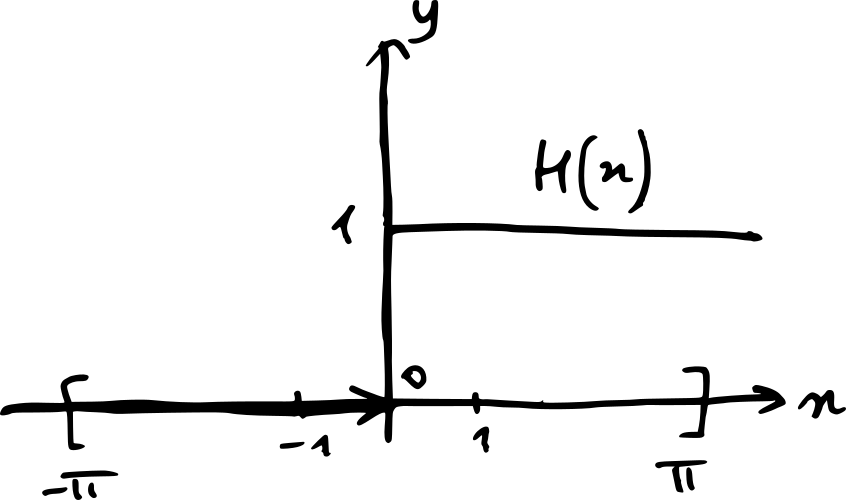
\includegraphics[width=0.25\textwidth]{09}
  \vspace{-4mm}
  \caption{Функция Хэвисайда}
\end{wrapfigure}

\textbf{Пример:} Функция Хэвисайда $H(x) = \begin{cases} 1, & x \geq 0 \\ 0, & x < 0 \end{cases}$ удовлетворяет условиям существования ряда Фурье. Ряд Фурье функции:
\[H(x) \sim \frac{a_0}{2} + \sum_{n=1}^{\infty} (a_n \cos nx + b_n \sin nx) \]
\[a_n = \frac{1}{\pi} \int \limits_{-\pi}^{\pi} H(x) \cos nx \di x = \frac{1}{\pi} \int \limits_{0}^{\pi} \cos nx \di x = \frac{1}{n\pi} \sin nx |^{\pi}_0, \quad n>0 \]
\[a_0 = \frac{1}{\pi} \int \limits_{-\pi}^{\pi} H(x) \di x = \frac{1}{\pi} \int \limits_{0}^{\pi} \di x = \frac{1}{\pi} x |^{\pi}_0 = 1, \quad n=0 \]
\[b_n = \frac{1}{\pi} \int \limits_{-\pi}^{\pi} H(x) \sin nx \di x = \frac{1}{\pi} \int \limits_{0}^{\pi} \sin nx \di x = \frac{1}{\pi} \left( -\frac{\cos nx}{n} \right) |^{\pi}_0 = \frac{1}{n\pi} (\cos n\pi - \cos 0) = \]
\[= \frac{1}{n\pi} (1-\cos n\pi) = \frac{2}{\pi (2k+1)}, \quad n = 2k+1, \quad k \geq 0 \]
Тогда ряд Фурье функции $H(x)$ имеет вид:
\[\tfrac{1}{2} + \sum_{k=0}^{\infty} \frac{2}{\pi (2k+1)} \sin (2k+1) \]

\subsection{Виды сходимости рядов Фурье}

Как известно, ряды Фурье как функциональные ряды могут сходиться поточечно или равномерно на $[-\pi, \pi]$. Но для рядов Фурье существует ещё один вид сходимости, \textit{сходимость в среднем} или \textit{сходимость по площадям}.

Ряд $\sum_{n=1}^{\infty} f_n(x)$ \textbf{сходится поточечно} на множестве $\irv{a, b} \subseteq \mathbb{R}$, если $\forall x \in \irv{a, b}$ числовой ряд $\sum_{n=1}^{\infty} f_n(x)$ сходится.

Ряд $\sum_{n=1}^{\infty} f_n(x)$ \textbf{сходится равномерно} на множестве $I = \irv{a, b} \subseteq \mathbb{R}$ к функции $f(x)$, если последовательность частичных сумм ряда $\{S_n(x) \}_{n \geq 1}$ сходится к ней равномерно на множестве $\irv{a, b} \subseteq \mathbb{R}$, то есть:
\[\forall \varepsilon > 0 \quad \exists N(\varepsilon), \quad \forall n>N(\varepsilon), \forall x \in I \quad \Rightarrow \quad |S_n(x) - f(x)|<\varepsilon \Leftrightarrow |R_n(x)|<\varepsilon \]

\begin{figure}[h]
 \centering
 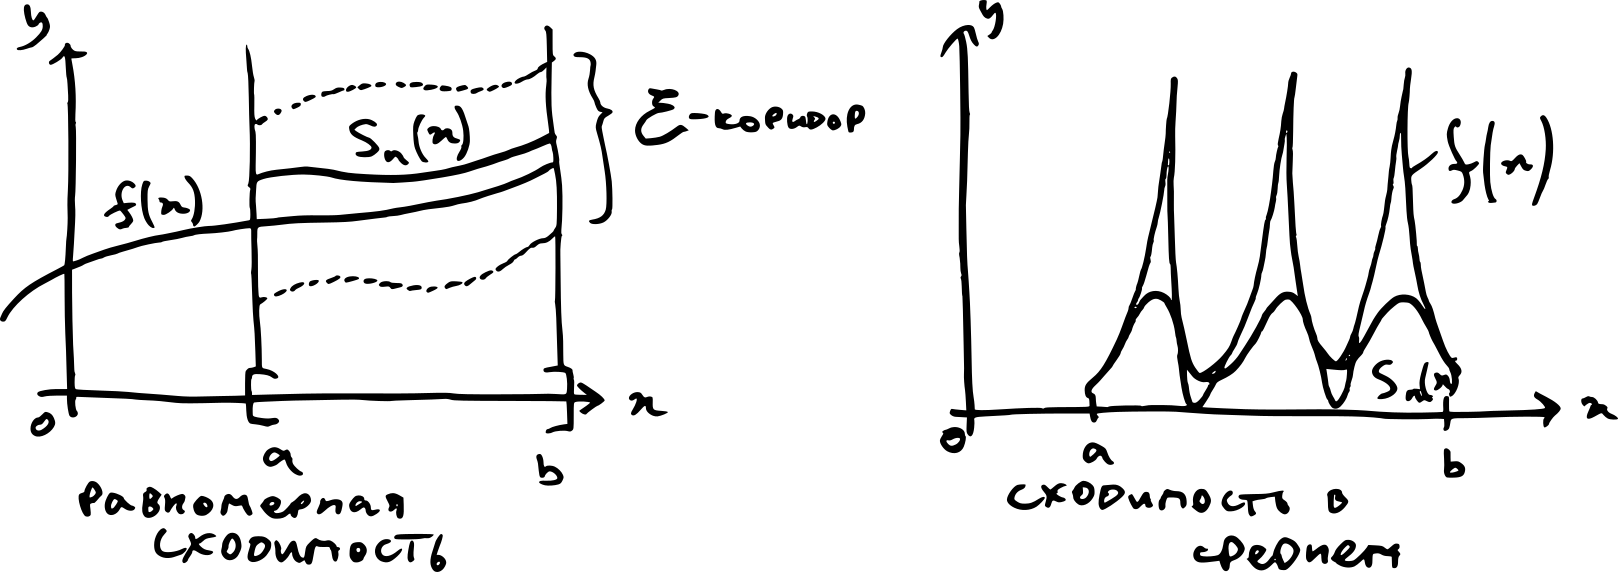
\includegraphics[width=0.6\textwidth]{10}
 \vspace{-4mm}
  \caption{Виды сходимости рядов Фурье}
\end{figure}

Ряд $\sum_{n=1}^{\infty} f_n(x)$ \textbf{сходится в среднем} на множестве $\irv{a, b} \subseteq \mathbb{R}$ к функции $f(x)$, интегрируемой со своим квадратом на интервале $\irv{a, b} \subseteq \mathbb{R}$, если $||f(x) - S_n(x)|| \xrightarrow[n \to +\infty]{} 0 $.

Геометрический смысл \textit{сходимости в среднем} состоит в том, что площадь подграфика разности $||f(x) - S_n(x)||$ стремится к нулю с ростом $n$ при возможной сколь угодно большой разности в отдельных точках. В отличие от равномерной сходимости, когда на всём интервале для любых $x \in \irv{a, b}$ значения частичных сумм $S_n(x)$ находятся в $\varepsilon$-коридоре от предельной функции $f(x)$.

\subsection{Достаточные условия поточечной сходимости}

\textbf{Теорема Дирихле} (без док-ва) \textbf{:} Если $f(x)$ задана на $[-\pi, \pi]$ и удовлетворяет условиям Дирихле:
\begin{enumerate}
 \item кусочно-непрерывная на отрезке $[-\pi, \pi]$, то есть имеет конечное число разрывов I-ого рода;
 \item имеет конечное количество экстремумов;
 \item интегрируема со своим квадратом на отрезке $[-\pi, \pi]$,
\end{enumerate}
тогда ряд Фурье функции $f(x) \sim \frac{a_0}{2} + \sum_{n=1}^{\infty} (a_n \cos nx + b_n \sin nx)$ сходится в точках \textit{непрерывности к функции} $f(x)$, а в точке \textit{разрыва} $x_0$ сходится \textit{к полусумме} односторонних пределов $\frac{f(x_{0-0}) - f(x_{0+0})}{2}$, где $f(x_{0 \pm 0}) = \lim_{x \to x_{0 \pm 0}} f(x)$.

\textbf{Примеры:} $D(x) = \begin{cases} 1, & x \in \mathbb{Q} \\ 0, & x \notin \mathbb{Q} \end{cases}$ (функция Дирихле) не годится, ибо имеет бесконечное число точек разрыва. $f(x) = \sin \frac{1}{x}$ также не годится, так как имеет бесконечное число экстремумов. $f(x) = \frac{1}{\sqrt{x}}$ не интегрируемая с квадратом на интервале $(0, 1)$.

\begin{figure}[h]
 \centering
 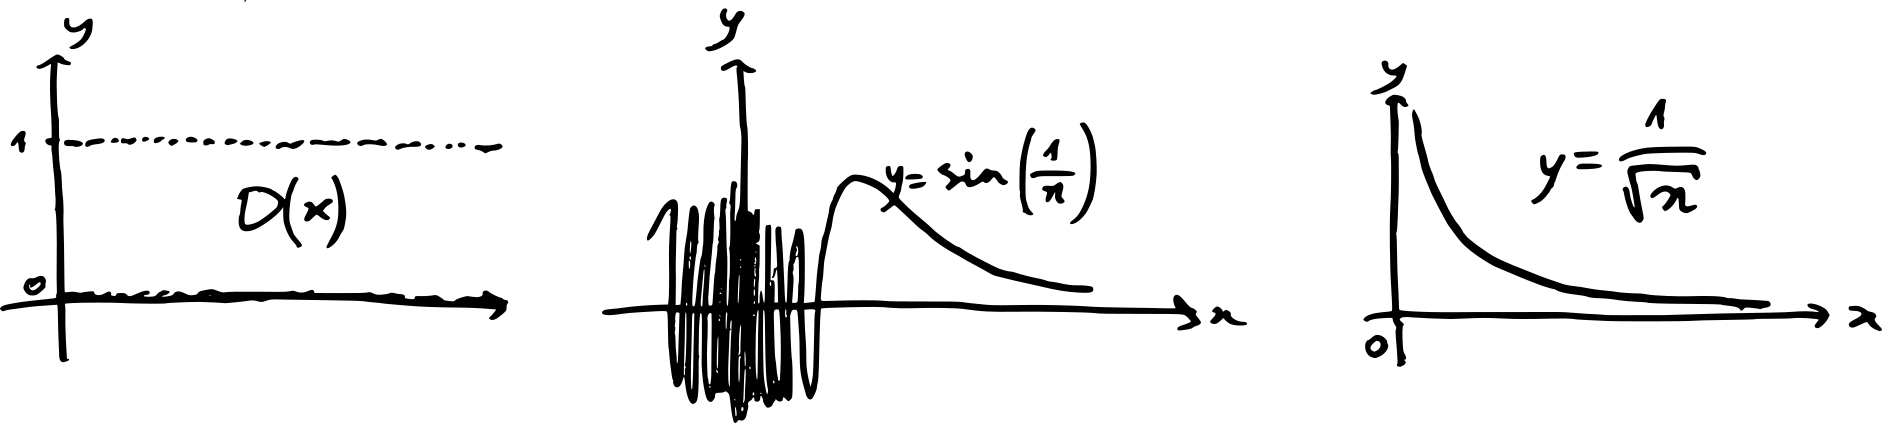
\includegraphics[width=0.65\textwidth]{11}
 \vspace{-4mm}
 \caption{Функции, не удовлетворяющие условиях Дирихле}
\end{figure}

\subsection{Периодическое продолжение функции}

Функция $F(x), \quad x \in \mathbb{R}$, равная ряду Фурье функции $f(x)$ на интервале $[-\pi, \pi]$, называется \textbf{периодическим продолжением} функции $f(x)$ с интервала $[-\pi, \pi]$.

Периодическое продолжение $F(x)$ - $2\pi$-периодическая функция. Ряд Фурье вырезает кусок и периодически его продолжает. В точках непрерывности сходится к функции, а в точках разрыва I-ого рода сходится к среднему значению функции.

\begin{figure}[h]
 \centering
 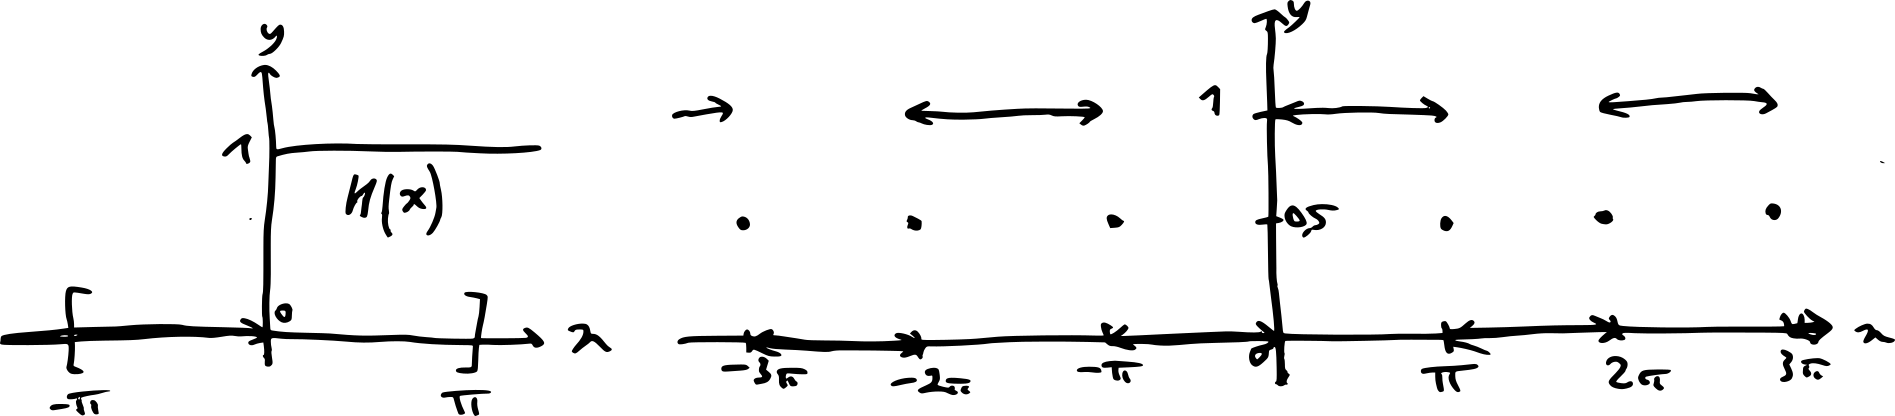
\includegraphics[width=0.7\textwidth]{12}
 \vspace{-4mm}
 \caption{Периодическое продолжение функции Хэвисайда}
\end{figure}

Функция Хэвисайда $H(x) = \begin{cases} 1, & x \geq 0 \\ 0, & x < 0 \end{cases}$ имеет ряд Фурье, равный $\tfrac{1}{2} + \sum_{k=0}^{\infty} \frac{2}{\pi (2k+1)} \cdot$ $\cdot \sin (2k+1)$, то есть периодическое продолжение функции $H(x)$ с интервала $[-\pi, \pi]$ на всю ось. По теореме Дирихле график периодического продолжения имеет вид как на \textit{Рис. 12}. Ряд Фурье вырезает кусок графика исходной функции с интервала $[-\pi, \pi]$ и его периодически продолжает. В точках непрерывности сходится к функции, а в точках разрыва I-ого рода (здесь это концы интервала $[-\pi, \pi]$) сходится к среднему значению односторонних пределов функции $H(x)$, равному $\tfrac{1}{2}$.

\subsection{Достаточные условия равномерной сходимости рядов Фурье}

\textbf{Теорема} (без док-ва) \textbf{:} Если функция $f(x)$ непрерывна на интервале $[-\pi, \pi]$ и $f(\pi) = f(-\pi)$. Тогда ряд Фурье сходится к функции $f(x)$ равномерно и абсолютно на интервале $[-\pi, \pi]$.

\begin{wrapfigure}{r}{0.25\textwidth}
  \centering
  \vspace{-13mm}
  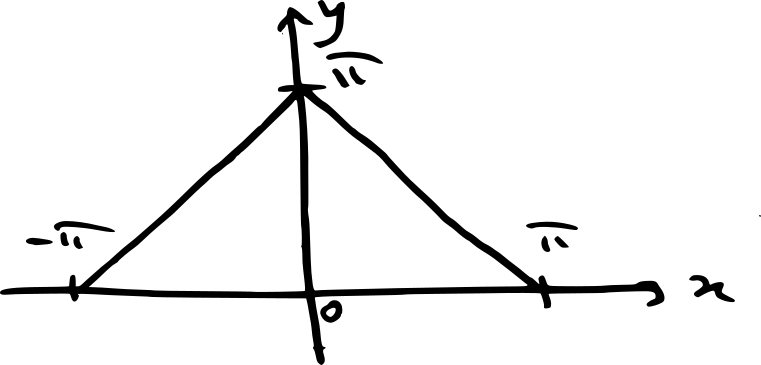
\includegraphics[width=0.25\textwidth]{13}
  \vspace{-6mm}
  \caption{Функция с равномерно и абсолютно сходящимся рядом Фурье}
\end{wrapfigure}

\textbf{Пример:} Функция $f(x) = \begin{cases} x+\pi, & x \in [-\pi, 0] \\ \pi - x, & x \in [0, \pi] \end{cases}$ чётная на интервале $[-\pi, \pi]$ следовательно, $[-\pi, \pi] \Rightarrow b_n=0$ и $a_n = \frac{2}{\pi} \int \limits_0^{\pi} f(x) \cos nx \di x \Rightarrow a_0 = \frac{2}{\pi} \int \limits_0^{\pi} (\pi - x) \di x = \frac{2\pi}{2} = \pi$.
\[a_n = \frac{2}{\pi} \int \limits_0^{\pi} (\pi - x) \cos nx \di x = \frac{2}{\pi} \left[ \pi \int \limits_0^{\pi} \cos nx \di x - \int \limits_0^{\pi} x \cos nx \di x \right] = \]
\[= \frac{2}{\pi} \cdot \frac{\pi \sin nx}{n} |^{\pi}_0 = -\frac{2}{\pi} \int \limits^{\pi}_0 x \cos nx \di x = \begin{Bmatrix} f(x) = x & f'(x) = 1 \\ g'(x) = \cos nx & g(x) = \tfrac{\sin nx}{n} \end{Bmatrix} = \]
\[= -\frac{2}{\pi} \cdot x \cdot \frac{\sin nx}{n} |^{\pi}_0 + \frac{2}{\pi} \int \limits_0^{\pi} \frac{\sin nx}{n} \di x = \frac{2}{n\pi} \left( -\frac{\cos nx}{n} \right) |_0^{\pi} = \frac{2}{n^2\pi} (1-\cos n\pi) = \frac{2 \cdot 2}{\pi (2k+1)^2} \]
В этом выражении $n = 2k+1, \quad k \geq 0$. Ряд Фурье функции:
\[f(x) \sim F(x) = \pi + \sum_{k=0}^{\infty} \frac{4}{\pi (2k+1)^2} \cos (2k+1)x \]
Ряд Фурье здесь сходится по признаку Вейерштрасса равномерно и абсолютно на всей оси.

\textbf{Замечание:} Имеет место теорема об оценке коэффициентов ряда Фурье. Если $f(x)$ - $k$-раз дифференцируемая функция на интервале $[-\pi, \pi]$ и периодическая с периодом $T=2\pi$, и $|f^k(x)|<M$ - ограничена на интервале $[-\pi, \pi]$. Тогда можно показать, что коэффициенты ряда Фурье $|a_n| < \frac{M}{n^{k+1}}$ и $|b_n| < \frac{M}{n^{k+1}}$.

\subsection{Достаточные условия сходимости в среднем}

\textbf{Теорема:} Если $f(x)$ задана и интегрируема со своим квадратом на интервале $[-\pi, \pi]$, тогда её ряд Фурье сходится к функции $f(x)$ в среднем, то есть $||f(x) - S_n(x)|| \xrightarrow[n \to +\infty]{} 0$, где:
\[S_n(x) = \frac{a_0}{2} + \sum_{k=1}^{n} (a_k \cos kx + b_k \sin kx) \]

\subsection{Ряд Фурье на произвольном интервале $[a, b]$}

Можно ввести аналогичную процедуру для произвольной функции и произвольного интервала. Пусть $f(x)$ задана и интегрируема со своим квадратом на интервале $[a, b]$. Построим отображение этого интервала на интервал $[-\pi, \pi]$:

\begin{figure}[h]
 \centering
 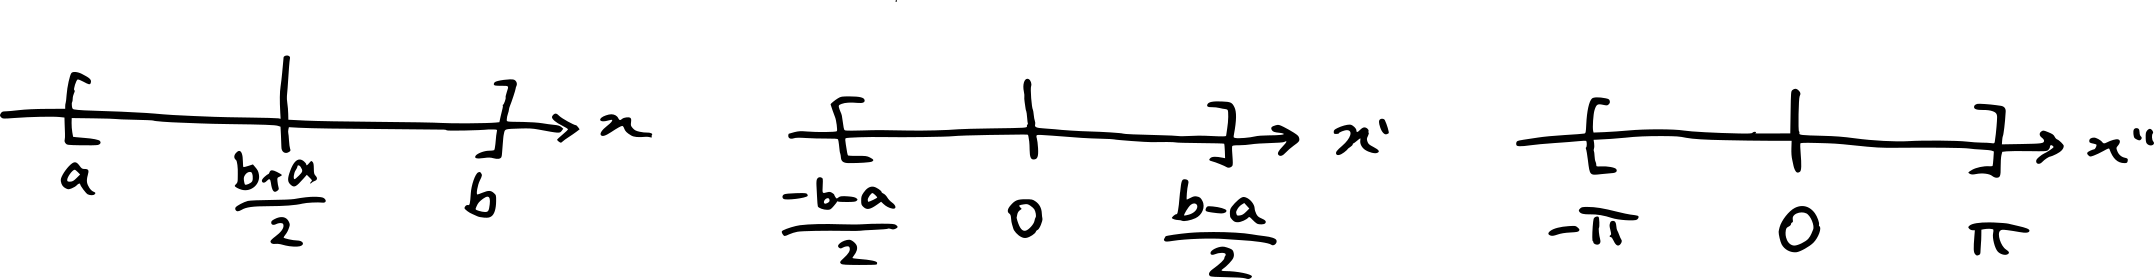
\includegraphics[width=0.7\textwidth]{14}
 \vspace{-4mm}
  \caption{Преобразования отрезка $[a,b]$}
\end{figure}

\[x' = x - \frac{a+b}{2} \in \left[ -\frac{b-a}{2}, \frac{b-a}{2} \right] \]
\[x^{\prime \prime} = \frac{2\pi}{b-a} x' = \frac{2\pi}{b-a} \left( x - \frac{a+b}{2} \right) \in \left[ -\frac{2\pi}{b-a} \frac{b-a}{2}, \frac{2\pi}{b-a} \frac{b-a}{2} \right] = [-\pi, \pi] \]
Тогда для $x \in [a, b]$ имеем $x^{\prime \prime} = \frac{2\pi}{b-a} \left( x - \frac{a+b}{2} \right) \in [-\pi, \pi]$. Соответственно, ряд Фурье для функции $f(x)$ на интервале $[a, b]$ будет иметь вид:
\[\frac{a_0}{2} + \sum_{n=1}^{\infty} \left[ a_n \cos \left( \frac{2\pi n}{b-a} \left( x - \frac{a+b}{2} \right) \right) + b_n \sin \left( \frac{2\pi n}{b-a} \left( x - \frac{a+b}{2} \right) \right) \right] \]
\[a_n = \frac{2}{b-a} \int \limits_a^b f(x) \cos \left( \frac{2\pi n \left( x - \frac{b+a}{2} \right)}{b-a} \right) \di x \]
\[b_n = \frac{2}{b-a} \int \limits_a^b f(x) \sin \left( \frac{2\pi n \left( x - \frac{b+a}{2} \right)}{b-a} \right) \di x \]

Тогда вид графика $y = F(x)$ - периодического продолжения функции $f(x)$ с интервала $[a, b]$ на действительную ось будет выглядеть следующим образом.

\begin{figure}[h]
 \centering
 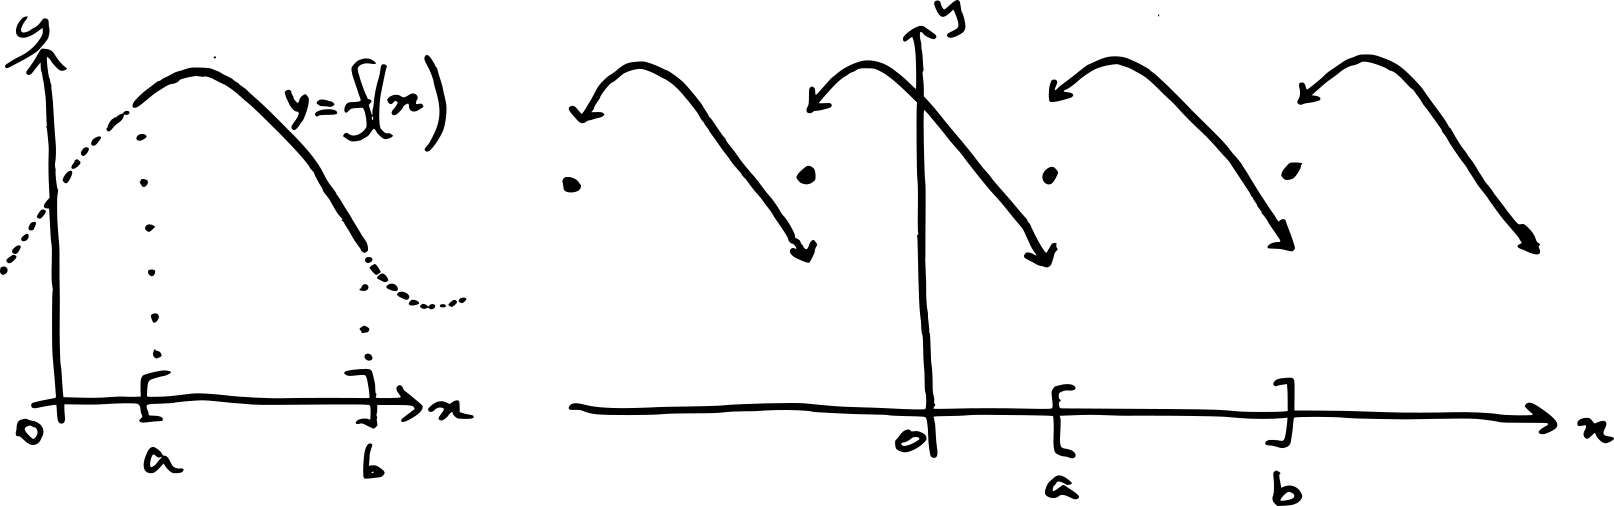
\includegraphics[width=0.7\textwidth]{15}
 \vspace{-4mm}
  \caption{Периодическое продолжение с отрезка $[a,b]$}
\end{figure}

\subsection{Ряд Фурье на произвольном симметричном интервале $[-l, l]$}

Частный случай произвольного интервала при $a = -l$ и $b = l$. Пусть $f(x)$ задана и интегрируема с квадратом на $[-l, l]$. Тогда её ряд Фурье примет вид:
\[f(x) \sim \frac{a_0}{2} + \sum_{n=1}^{\infty} \left[ a_n \cos \frac{\pi}{l} nx + b_n \sin \frac{\pi}{l} nx \right] \]
\[a_n = \frac{1}{l} \int \limits_{-l}^l f(x) \cos \frac{n\pi x}{l} \di x \]
\[b_n = \frac{1}{l} \int \limits_{-l}^l f(x) \sin \frac{n\pi x}{l} \di x \]
Соответственно, график периодического продолжения будет периодически продолжать график исходной функции с интервала $[-l, l]$ на всю действительную ось.

\subsection{Общие свойства рядов Фурье: неравенства Буняковского и Бесселя}

Ниже пойдет речь о свойствах произвольной системы ортогональных функций, не только тригонометрических.

\subsubsection{Неравенство Буняковского}

Если функции $f(x)$ и $g(x)$ - интегрируемые со своим квадратом на отрезке $[a, b]$, тогда:
\[\left( \int \limits_a^b f(x) g(x) \di x \right)^2 \leq \int \limits_a^b f^2(x) \di x \cdot \int \limits_a^b g^2(x) \di x \]

\textbf{Док-во:} Элементарное неравенство $(f(x) - g(x))^2 \geq 0$ эквивалентно следующему:
\[f(x) g(x) \leq \tfrac{1}{2} (f^2(x) + g^2(x)) \]
Из последнего следует интегрируемость произведения функций $f(x) g(x)$. Из свойств определённого интеграла имеем:
\[\int \limits_a^b (f + \lambda g)^2 \di x = \underbrace{\int \limits_a^b f^2(x) \di x}_A + 2\lambda \underbrace{\int \limits_a^b f(x) g(x) \di x}_B + \lambda^2 \underbrace{\int \limits_a^b g^2(x) \di x}_C = A + 2\lambda B + \lambda^2 C \geq 0, \quad \forall \lambda \]
\[\Updownarrow \]
\begin{center}
\textbf{ВЫРАЖЕНИЕ ПОД ВОПРОСОМ!}
\end{center}
\[D = B^2 - AC \leq 0 \quad \Leftrightarrow \quad B^2 \leq AC \quad \Leftrightarrow \quad \left( \int \limits_a^b f(x) g(x) \di x \right)^2 \leq \underbrace{\int \limits_a^b f^2(x) \di x}_{< +\infty} \underbrace{\int \limits_a^b g^2(x) \di x}_{< +\infty} < +\infty \]
Кроме этого:
\[\int \limits_a^b (f(x)+g(x))^2 \di x = \int \limits_a^b f^2(x) \di x + 2\int \limits_a^b f(x) g(x) \di x + \int \limits_a^b g^2(x) \di x < +\infty \]
\textit{Таким образом, произведение и сумма функций, интегрируемых со своим квадратом, также принадлежит этому же классу функций.}

\subsubsection{Неравенство Бесселя}

Если $f(x)$, функция интегрируемая со своим квадратом на отрезке $[a, b]$, а $\{\varphi_k(x) \}_{k \geq 0}$ - система ортогональных функций на отрезке $[a, b]$, и разложение в ряд Фурье $f(x) = \sum_{k=0}^{+\infty} c_k \varphi_k(x)$, тогда:
\[\int \limits_a^b f^2(x) \di x \geq \sum_{k=0}^n c^2_k ||\varphi_k(x)||^2 \]

\textbf{Док-во:} Если $f(x) = \sum_{k=0}^n c_k \varphi_k(x)$, то $\int \limits_a^b f(x) \varphi_k(x) \di x = c_k \cdot ||\varphi_k(x)||^2$. Покажем, что квадратичное отклонение функции $f(x)$ от частичной суммы вида $\sigma_n(x) = \sum_{k=0}^n \gamma_k \varphi_k(x)$ будет минимальным при $c_k = \gamma_k, \quad k = 0, 1, \cdots$. Действительно, скалярное произведение в силу ортогональности $\{\varphi_k(x) \}_{k \geq 0}$ равно:
\[\int \limits_a^b f(x) \sigma_n(x) \di x = \sum_{k=0}^n c_k \gamma_k ||\varphi_k(x)||^2 \hspace{1cm} \int \limits_a^b \sigma^2_n(x) \di x = \sum_{k=0}^n \gamma^2_k ||\varphi_k(x)||^2 \]
Тогда квадратичное отклонение будет равно:
\[\int \limits_a^b (f(x) - \sigma_n(x))^2 \di x = \int \limits_a^b f^2(x) \di x - 2\int \limits_a^b f(x) \sigma_n(x) \di x + \int \limits_a^b \sigma_n^2(x) \di x = \]
\[= \int \limits_a^b f^2(x) \di x - 2\sum_{k=0}^n c_k \gamma_k ||\varphi_k(x)||^2 + \sum_{k=0}^n \gamma^2_k ||\varphi_k(x)||^2 = \]
\[= \underbrace{\int \limits_a^b f^2(x) \di x}_{\const} + \sum_{k=0}^n (c_k - \gamma_k)^2 ||\varphi_k(x)||^2 - \sum_{k=0}^n \underbrace{c^2_k ||\varphi_k(x)||^2}_{\const} \to \min \]
Тогда:
\[\min \left[ \underbrace{\int \limits_a^b f^2(x) \di x}_{\const} + \sum_{k=0}^n (c_k - \gamma_k)^2 ||\varphi_k(x)||^2 - \sum_{k=0}^n \underbrace{c^2_k ||\varphi_k(x)||^2}_{\const} \right] = \int \limits_a^b f^2(x) \di x - \sum_{k=0}^n c^2_k ||\varphi_k(x)||^2 \]
при $c_k = \gamma_k, \quad k = 0, 1, \cdots$

Отсюда следует \textit{неравенство Бесселя}, так как $\int \limits_a^b (f(x) - \sigma_n(x))^2 \di x \geq 0$, то:
\[\int \limits_a^b f^2(x) \di x \geq \sum_{k=0}^n c^2_k ||\varphi_k(x)||^2 \]

\textbf{Следствия:}
\begin{enumerate}
 \item \textit{Сумма ряда Фурье функции, интегрируемой со своим квадратом, сходится}, так как правая часть неравенства $\int \limits_a^b f^2(x) \di x \geq \sum_{k=0}^n c^2_k ||\varphi_k(x)||^2$ монотонно возрастает при $n \to +\infty$, остаётся ограниченной левой частью (по теореме Вейерштрасса о пределе монотонной функции), то есть:
 \[\int \limits_a^b f^2(x) \di x = \sum_{k=0}^{+\infty} c^2_k ||\varphi_k(x)||^2 \]
 \item Из сходимости ряда Фурье при $n \to +\infty$ следует, что $c_n ||\varphi_n(x)||^2 \xrightarrow[n \to +\infty]{} 0$, или в случае ортонормированной системы, когда коэффициенты ряда Фурье $c_n \xrightarrow[n \to +\infty]{} 0$ стремятся к нулю и $\int \limits_a^b f^2(x) \di x = \sum_{k=0}^{+\infty} c^2_k$.
\end{enumerate}

\subsection{Полнота системы функций}

Свойство полноты системы функций означает, что, пользуясь аналогией с конечномерным векторным пространством, ортогональная система функций является \textit{базисом} для пространства функций, интегрируемых с полным квадратом, то есть любая функция представима рядом Фурье всюду кроме конечного числа точек.

\textit{Система ортогональных функций} $\{\varphi_n(x) \}_{n \geq 0}$ называется \textbf{полной}, если для любой функции $f(x)$, интегрируемой со своим квадратом, имеет место равенство для ряда Фурье по этой системе:
\[\int \limits_a^b f^2(x) \di x = \sum_{k=0}^{+\infty} c^2_k ||\varphi_k(x)||^2 \]

\textbf{Критерий полноты системы:} Система функций полна тогда и только тогда, когда для любой функции $f(x)$, интегрируемой со своим квадратом, имеет место равенство для ряда Фурье по этой системе функций:
\[\lim_{n \to +\infty} \int \limits_a^b \left[ f(x) - \sum_{k=0}^n c_k \varphi_k(x) \right]^2 \di x = 0 \]

\textbf{Док-во:} В доказательстве неравенства Бесселя мы получили равенство для минимального квадратичного отклонения:
\[\int \limits_a^b \left[ f(x) - \sum_{k=0}^n c_k \varphi_k(x) \right]^2 \di x = \int \limits_a^b f^2(x) \di x - \sum_{k=0}^n c^2_k ||\varphi_k(x)||^2 \]
Переходя к пределу при $n \to +\infty$, получим условие равносильности утверждений о полноте системы и сходимости ряда Фурье в среднем к функции $f(x)$.

Таким образом для полноты системы необходимо и достаточно, чтобы ряд Фурье для любой функции $f(x)$, интегрируемой со своим квадратом, сходился к ней в среднем.

\textbf{Следствие:} В силу полноты системы тригонометрических функций (\textit{см. док-во, например, Толстов Г.П. Ряды Фурье., 3-е издание – М.: Наука 1980}) ряд Фурье для любой функции $f(x)$, интегрируемой со своим квадратом, сходится к ней в среднем.

\textbf{Свойства полных систем} (без док-ва) \textbf{:}
\begin{enumerate}
 \item Если система функций полна, то непрерывная функция, ортогональная ко всем функциям системы равна тождественному нулю.
 \item Если система непрерывных функций полна, и ряд Фурье для непрерывной функции $f(x)$ сходится равномерно, то его сумма равна $f(x)$.
 \item Если система функций полна, и ряд Фурье для любой функции $f(x)$, интегрируемой со своим квадратом, можно интегрировать почленно, независимо от того, сходится он или нет.
\end{enumerate}

\section{Интеграл Фурье и интегральные преобразования Фурье}

Для тех случаев, когда функция $f(x)$ периодическая и принадлежит к достаточно широкому классу функций, интегрируемых со своим квадратом, ряд Фурье достаточно точно её представляет для любого сколь угодно большого периода. Если период устремить к бесконечности, то тогда мы будем иметь дело с представлением непериодической функции, и ряд Фурье превратится в интеграл Фурье, который в свою очередь можно представить как двойное интегральное преобразование.

\subsection{Интеграл Фурье}

Пусть $f(x)$ задана и интегрируема со своим квадратом на $(-\infty, \infty)$. Тогда для неё $\forall l > 0$ существует ряд Фурье на $[-l, l]$:
\[f(x) \sim \frac{a_0}{2} + \sum_{n=1}^{+\infty} \left[ a_n \cos \frac{\pi nx}{l} + b_n \sin \frac{\pi nx}{l} \right] \]
\[a_n = \frac{1}{l} \int \limits_{-l}^l f(x) \cos \frac{\pi nx}{l} \di x \quad n=0,1,2,\cdots \hspace{1 cm} a_n = \frac{1}{l} \int \limits_{-l}^l f(x) \cos \frac{\pi nx}{l} \di x \quad n=1,2,\cdots \]
Подставим $a_n$ и $b_n$ в ряд Фурье:
\[f(x) \sim \frac{a_0}{2} + \sum_{n=1}^{+\infty} \left[ a_n \cos \frac{\pi nx}{l} + b_n \sin \frac{\pi nx}{l} \right] = \frac{1}{2l} \int \limits_{-l}^l f(t) \di t + \sum_{n=1}^{+\infty} \frac{1}{l} \int \limits_{-l}^l \left( f(t) \cos \frac{\pi nt}{l} \cos \frac{\pi nx}{l} + \right. \]
\[\left. + f(t) \sin \frac{\pi nt}{l} \sin \frac{\pi nx}{l} \right) \di t = \frac{1}{2l} \int \limits_{-l}^l f(t) \di t + \sum_{n=1}^{+\infty} \frac{1}{l} \int \limits_{-l}^l \cos \frac{\pi n(x-t)}{l} f(t) \di t \]
Введём частоту $\omega_n \equiv \frac{\pi n}{l}$ и $\Delta \omega_n = \omega_n - \omega_{n-1} = \frac{\pi}{l}$. Тогда получим:
\[f(x) = \frac{1}{2l} \int \limits_{-l}^l f(t) \di t + \frac{1}{\pi} \sum_{n=1}^{\infty} \Delta \omega_n \int \limits_{-l}^l \cos \omega_n (x-t) f(t) \di t = \]
\[= \frac{1}{2l} \int \limits_{-l}^l f(t) \di t + \frac{1}{\pi} \sum_{n=1}^{\infty} \int \limits_{-l}^l \cos \omega_n (x-t) f(t) \di t \Delta \omega_n = \]
\[= \begin{Bmatrix} \textrm{ Переход к пределу } l \to +\infty \Rightarrow \Delta \omega_n \to 0; \omega_n \to \omega \\ \frac{1}{2l} \int \limits_{-l}^l f(t) \di t \xrightarrow[l \to +\infty]{} 0 \textrm{ так как: } \left| \int \limits_{-l}^l f(t) \di t \right| < +\infty \end{Bmatrix} = \]
\[= \frac{1}{\pi} \int \limits_0^{+\infty} \int \limits_{-\infty}^{\infty} \cos \omega (x-t) f(t) \di t \di \omega - \textbf{косинус-интеграл Фурье.} \]
Раскрыв косинус и проинтегрировав по $t$, получим формулу, напоминающую ряд Фурье:
\[f(x) = \frac{1}{\pi} \int \limits_0^{+\infty} (a(\omega) \cos \omega x + b(\omega) \sin \omega x) \di \omega \]
\[a(\omega) = \frac{1}{\pi} \int \limits_{-\infty}^{\infty} f(t) \cos \omega t \di t \hspace{1cm} b(\omega) = \frac{1}{\pi} \int \limits_{-\infty}^{\infty} f(t) \sin \omega t \di t \]

\subsection{Косинус- и синус-преобразование Фурье для чётных и нечётных функций}

Если $f(x)$ чётная функция на $(-\infty, +\infty)$, тогда из косинус-интеграла Фурье по формуле сложения получим:
\[f(x) = \frac{1}{\pi} \int \limits_0^{+\infty} \int \limits_{-\infty}^{+\infty} [\cos \omega x \cos \omega t + \sin \omega x \sin \omega t] f(t) \di t \di \omega = \]
\[= \frac{1}{\pi} \int \limits_0^{+\infty} \left[ \int \limits_{-\infty}^{\infty} \underbrace{\cos \omega x \cos \omega t \cdot f(t)}_{\textrm{чётная по } t} \di t + \int \limits_{-\infty}^{\infty} \underbrace{\sin \omega x \sin \omega t \cdot f(t)}_{\textrm{нечётная по } t} \di t \right] \di \omega = \]
\[= \frac{2}{\pi} \int \limits_0^{+\infty} \int \limits_0^{+\infty} \cos \omega x \cos \omega t \cdot f(t) \di t \di \omega - \textbf{косинус-преобразование для чётных функций.} \]

Аналогично, для нечётной функции $f(x)$ получим:
\[\frac{2}{\pi} \int \limits_0^{+\infty} \int \limits_0^{+\infty} \sin \omega x \sin \omega t \cdot f(t) \di t \di \omega - \textbf{синус-преобразование для нечётных функций.} \]

\textbf{Замечание:} Если $f(x)$ задана на интервале $(0, +\infty)$, то её косинус-преобразование задаёт \textit{чётное} продолжение по $x$ на $(-\infty, +\infty)$, а её синус преобразование - \textit{нечётное} продолжение по $x$ на $(-\infty, +\infty)$.

\begin{figure}[h]
 \centering
 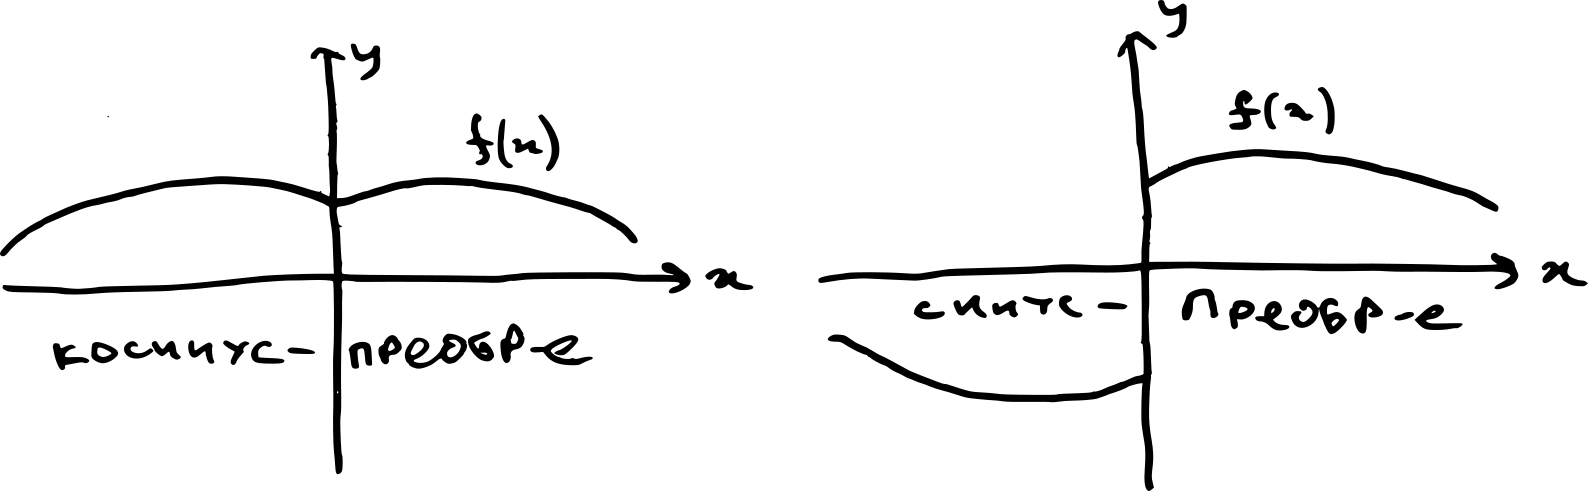
\includegraphics[width=0.7\textwidth]{16}
 \vspace{-4mm}
  \caption{Косинус- и синус-преобразования}
\end{figure}

\subsection{Интеграл Фурье в комплексной форме}

Обобщая на комплексную плоскость параметр $\omega$, получим интеграл Фурье в комплексной форме. Пусть $f(x)$ задана и интегрируема на $(-\infty, +\infty)$. Тогда имеет место косинус-интеграл Фурье:
\[f(x) = \frac{1}{\pi} \int \limits_0^{+\infty} \int \limits_{-\infty}^{+\infty} \cos (\omega (x-t)) f(t) \di t \di \omega \]
И заметим, что $\cos (\omega (x-t))$ - чётная функция по $\omega$, а $\sin (\omega (x-t))$ - нечётная. Тогда и внутренний интеграл в двойном интеграле $\int \limits_{-\infty}^{+\infty} \int \limits_{-\infty}^{+\infty} \sin (\omega (x-t)) f(t) \di t \di \omega = 0$ тоже является нечётной функцией по $\omega$, поэтому и повторный интеграл равен нулю. Аналогично, в силу чётности:
\[\int \limits_0^{+\infty} \int \limits_{-\infty}^{+\infty} \cos (\omega (x-t)) f(t) \di t \di \omega = \tfrac{1}{2} \int \limits_{-\infty}^{+\infty} \int \limits_{-\infty}^{+\infty} \cos (\omega (x-t)) f(t) \di t \di \omega \]
Тогда прибавим к интегралу Фурье выражение $\frac{i}{2 \pi} \int \limits_0^{+\infty} \int \limits_0^{+\infty} \sin (\omega (x-t)) f(t) \di t \di \omega = 0$. Получаем следующее:
\[f(x) = \frac{1}{2\pi} \int \limits_0^{+\infty} \int \limits_0^{+\infty} \{\cos (\omega (x-t)) f(t) \} \di t \di \omega + \frac{1}{2\pi} \int \limits_0^{+\infty} \int \limits_0^{+\infty} \{i \sin (\omega (x-t)) f(t) \} \di t \di \omega = \]
\[= \frac{1}{2\pi} \int \limits_0^{+\infty} \int \limits_0^{+\infty} \{\cos (\omega (x-t)) f(t) + i \sin (\omega (x-t)) f(t) \} \di t \di \omega = \frac{1}{2\pi} \int \limits_0^{+\infty} \int \limits_0^{+\infty} \mathrm{e}^{-i\omega (x-t)} f(t) \di t \di \omega \]

Итак, интеграл Фурье в комплексной форме: $f(x) = \frac{1}{2\pi} \int \limits_0^{+\infty} \int \limits_0^{+\infty} \mathrm{e}^{-i\omega (x-t)} f(t) \di t \di \omega$.

\subsection{Интегральные преобразования Фурье и формула его обращения}

Перепишем последний интеграл в следующем виде:
\[f(x) = \frac{1}{\sqrt{2\pi}} \int \limits_0^{+\infty} \frac{\mathrm{e}^{i\omega x}}{\sqrt{2\pi}} \left[ \int \limits_{-\infty}^{+\infty} f(t) \mathrm{e}^{-i\omega t \di t} \right] \di \omega \]
Если ввести функцию $F(\omega) = f^F(\omega) = \frac{1}{\sqrt{2\pi}} \int \limits_{-\infty}^{+\infty} f(t) \mathrm{e}^{-i\omega t} \di t$, называемую \textbf{интегральным преобразованием Фурье} с параметром преобразования $\omega$, тогда интеграл примет вид:
\[f(x) \frac{1}{\sqrt{2\pi}} \int \limits_{-\infty}^{+\infty} f^F(\omega) \mathrm{e}^{i\omega x} \di \omega \hspace{1cm} f^F(\omega) = \frac{1}{\sqrt{2\pi}} \int \limits_{-\infty}^{+\infty} f(t) \mathrm{e}^{-i\omega t} \di t \]

Первая формула - интеграл Фурье - представляет из себя формулу обратного преобразования Фурье, а вторая - прямого преобразования Фурье для функций, интегрируемых со своим квадратом.

\textbf{Замечание:} Так как преобразование Фурье применимо к сравнительно узкому классу функций, то чаще используют другое интегральное преобразование - преобразование Лапласа для функций, не более, чем экспоненциального роста. Оно обладает схожими свойствами и применяется для решения дифференциальных уравнений в частных производных.

\section{Введение в вариационное исчисление}

Под \textbf{вариационным исчислением} понимается методы определения экстремумов \textit{функционалов}, то есть отображений из пространства функций в поле $\mathbb{R}$. Типичным функционалом, притом линейным, является определённый интеграл. Задачи нахождения таких экстремумов называются \textit{вариационными задачами}.

\textit{Основная идея вариационного исчисления - это распространение понятий и методов дифференциального исчисления функции одной переменной на функционалы, рассматриваемые как <<функции>> от функций.}

\subsection{Классические примеры вариационных задач и их классификация}

\subsubsection{Задача о брахистохроне}

\begin{wrapfigure}{r}{0.2\textwidth}
  \centering
  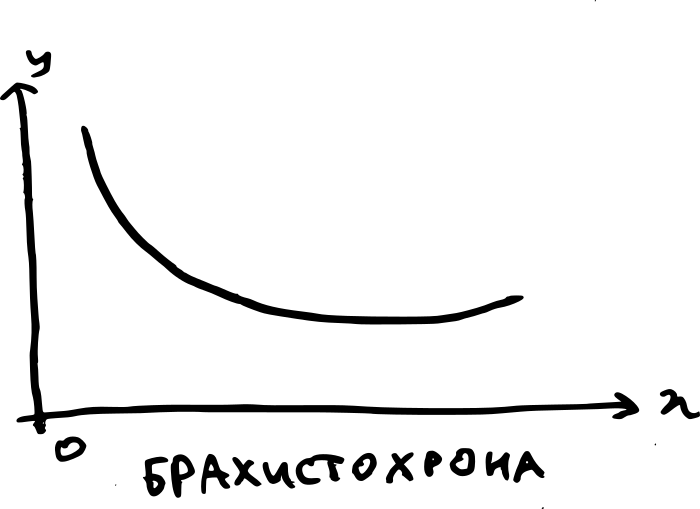
\includegraphics[width=0.2\textwidth]{17}
  \vspace{-4mm}
  \caption{Брахистохрона}
\end{wrapfigure}

В 1696 году Иоганн Бернулли предложил первую вариационную задачу - задачу о линии наискорейшего спуска - \textit{брахистохроне}. Заданы две материальные точки А и В, находящиеся на разных уровнях. По какой траектории
время спуска под действием силы тяжести будет наименьшим? Эту задачу решили Иоганн и Яков Бернулли, И. Ньютон, В.
Лейбниц. Решением оказалась кривая, под названием циклоида, кривая которую описывает точка окружности, катящейся по прямой.

\subsubsection{Изопериметрическая задача}

Требуется найти замкнутую линию, заданной длины $l$, ограничивающую максимальную площадь $S$. Решение этой известной ещё в Древней Греции задаче – \textit{окружность}, длиной $l$. В мифе об основании Карфагена Дидона, дочь тирского царя, после убийства своего мужа её братом, бежала в Африку. У нумедийского царя она купила столько земли, сколько могла покрыть воловья шкура. Хитроумная Дидона разрезала шкуру на тонкие полоски, связала их и огородила участок земли, достаточный для строительства города.

\begin{footnotesize}
\textbf{Примечание:} Известно примерное решение этой задачи Дидоны. Если шкура вола имеет площадь 4 кв. м разрезается на куски шириной 1 мм, то получается около 4 км шнура, которым можно огородить круг площадью около 1.3 кв. км, площадь вполне достаточную для строительства античного города.
\end{footnotesize}

Условия типа $l = \int \limits_a^b \sqrt{x^{\prime 2}(t) + y^{\prime 2}(t)} \di t \leq (\geq) L$ называются \textbf{изопериметрическими}. Общие методы решения вариационных задач с такими условиями были разработаны Л. Эйлером.

\subsubsection{Задача о геодезических линиях}

Пусть заданы две точки на поверхности $S$, требуется найти линию кратчайшей длины, соединяющей эти точки. Эти кратчайшие линии называются геодезическими. Частный случай этой задачи - прокладка кратчайших авиамаршрутов. Если поверхность $S$, заданная в неявном виде уравнением $\varphi (x, y, z) = 0$, то речь идёт о минимуме функционала $l = \int \limits_a^b \sqrt{1 + y^{\prime 2}(x) + z^{\prime 2}(x)} \di x$, где функции $y(x)$ и $z(x)$ должны удовлетворять условию $\varphi (x, y(x), z(x)) = 0$, то есть уравнению поверхности. Эта \textit{вариационная задача} на \textbf{условный} или \textbf{связанный экстремум}. Эта задача была решена в 1698 году Я. Бернулли, но общий метод решения такого рода задач был разработан Л. Эйлером и Ж. Лагранжем в XVIII веке.

Обобщая, можно сказать, что вариационная задача с неподвижными границами сводится к отысканию экстремума функционалов вида:
\[\int \limits_a^b F(x, y(x), y'(x)) \di x, \hspace{15mm} \int \limits_a^b F(x, y(x), y'(x), \cdots, y^{(n)}(x)) \di x, \]
\[\int \limits_a^b F(x, y_1(x), y_{1}'(x), \cdots, y_n(x), y_{n}'(x)) \di x \]
В случае, когда варьируются и пределы интегрирования, тогда \textit{получают вариационную задачу с подвижными границами}.

\subsection{Основные понятия вариационного исчисления}

Методы нахождения экстремума функционалов, <<функций от фунций>>, схожи с методами отыскания экстремумов функций. Введём параллельно аналогичные понятия для функций и функционалов.

\subsubsection{Основные классы функций и понятие метрики пространства}

\textbf{Класс} $C^0[a, b]$ - пространство непрерывных функций на отрезке $[a, b]$.

\textbf{Класс} $C^1[a, b]$ - пространство непрерывно дифференцируемых функций на отрезке $[a, b]$.

\textbf{Класс} $C^k[a, b]$ - пространство $k$ раз непрерывно дифференцируемых функций на отрезке $[a, b]$.

Для того, чтобы оценить близость, похожесть функций, вводят понятие \textit{расстояния} или \textit{метрики} в пространстве $C^k[a, b]$. Расстоянием между функциями $f(x)$ и $g(x)$ в пространстве функций $C^k[a, b]$ называется число, равное:
\[\rho_{C^k}(f, g) = \sum_{i=0}^k \max \limits_{x \in [a, b]} \left| f^{(i)}(x) - g^{(i)}(x) \right| \]

\textbf{Примеры:}
\begin{itemize}
 \item $f(x) = |x| \in C^0[a, b], \quad \forall [a, b] \subset \mathbb{R}, \textrm{но} f(x) = |x| \not\in C^1[-a, a]$ - непрерывная на любом интервале, но не на любом дифференцируемая.
 \item $f(x) = \mathrm{e}^x \in C^k[a, b], \quad \forall [a, b] \subset \mathbb{R}, \forall k \in \mathbb{N}$ - бесконечно дифференцируемая на любом интервале.
 \item Расстояние между функциями:
 \[\rho_{C^0[0, 1]}(x, x^2) = \max \limits_{x \in [0, 1]} \left| x - x^2 \right| = (x - x^2) |_{x=\tfrac{1}{2}} = \frac{1}{4} \]
 \[\rho_{C^1[0, 1]}(x, x^2) = \max \limits_{x \in [0, 1]} \left| x - x^2 \right| + \max \limits_{x \in [0, 1]} \left| (x)' - (x^2)' \right| = \frac{1}{4} + \max \limits_{x \in [0, 1]} |1-2x| = \frac{1}{4} + 1 = 1\tfrac{1}{4} \]
\end{itemize}

\subsubsection{Понятие функционала и область его задания}

\textbf{Функционал} $V$ - это отображение, действующее из множества функций $D = \{ f(x) \}$, где $D$ - область задания функционала из некоторого класса функций, во множество чисел $\mathbb{R}$. \textit{Обозначается}:
\[V: \quad D \to \mathbb{R}, \quad V = V(y(x)), \quad \textrm{где } y(x) \textrm{ из множества функций } D \subseteq C^k[a, b] \]

\textbf{Классом допустимых функций} называется множество функций, на которых определён функционал.

\textbf{Примеры функционалов:}
\begin{enumerate}
 \item $M = \max y(x), \quad x \in [a, b], y(x) \in C^0[a, b]$ - наибольшее значение функции на отрезке.
 \item $m = \min y(x), \quad x \in [a, b], y(x) \in C^0[a, b]$ - наименьшее значение функции на отрезке.
 \item $V(y(x)) = y(x_0), \quad x_0 \in [a, b], y(x) \in C^0[a, b]$ - значение функции в точке.
 \item $S = \int \limits_a^b y(x) \di x, \quad y(x) \in C^0[a, b]$ - значение площади подграфика от неотрицательной функции на отрезке $[a, b]$.
 \item $L = \int \limits_a^b \sqrt{1 + y^{\prime 2}(x)} \di x, \quad y(x) \in C^1[a, b]$ - значение длины кривой - графика дифференцируемой функции $y(x)$ на отрезке $[a, b]$.
\end{enumerate}

Функционал $L(y(x))$ называется \textbf{линейным}, если:
\begin{enumerate}
 \item $L(\lambda y(x)) = \lambda L(y(x)), \quad \forall y(x) \in D$;
 \item $L(y_1(x) + y_2(x)) = L(y_1(x)) + L(y_2(x)), \quad \forall y_1(x), y_2(x) \in D$.
\end{enumerate}

\textbf{Примеры:}
\begin{enumerate}
 \item В приведённых выше примерах 3 и 4 -- линейный функционалы, остальные нелинейные.
 \item $L(y(x)) = \int \limits_a^b (p(x)y(x) + q(x)y'(x)) \di x$ - линейный функционал.
\end{enumerate}

\subsubsection{Вариации аргумента функционала и понятие близости функций $k$-го порядка в определённом классе функций}

\textbf{Приращением} или \textbf{вариацией} аргумента $y(x)$ при $y_0(x)$ функционала $V(y_0(x)), \quad y_0(x) \in D$ называется функция вида $\delta y = y(x) - y_0(x)$, где $y(x)$ - произвольная функция в том же множестве функций $D$. Обозначается $\delta y$.

\begin{wrapfigure}[8]{l}{0.2\textwidth}
  \centering
  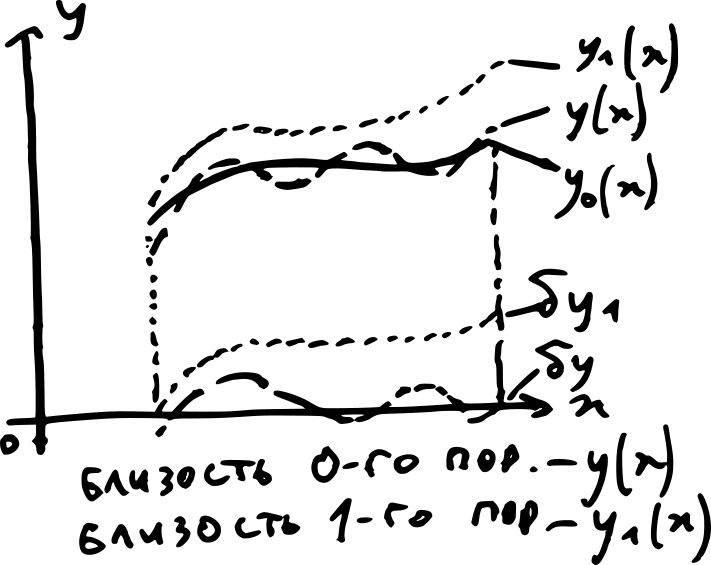
\includegraphics[width=0.2\textwidth]{20}
  \vspace{-4mm}
  \caption{Близости 0-го и 1-го порядков}
\end{wrapfigure}

Функция $y(x), \quad y(x) \in C^k[a, b]$, $\delta$-\textbf{близка} $y_0(x)$ в смысле \textbf{близости} $k$-\textbf{го порядка} на $[a, b]$, если:
\[\forall x \in [a, b] \Rightarrow \begin{cases} |y(x) - y_0(x)| < \delta \\ |y'(x) - y'_0(x)| < \delta \\ \cdots \\ |y^{(k)}(x) - y_0^{(k)}(x)| < \delta \\ \end{cases} \]

\textbf{Пример:} Близость 0-го порядка к $y_0(x)$ - разность значений в $\delta$-коридоре $(y(x))$. Близость 1-го порядка к $y_0(x)$ - разность значений и функций, и их первых производных в $\delta$-коридоре.

\subsubsection{Аналогия понятий приращения, непрерывности, вариации функционала с этими понятиями для функции}

Сведём все основные аналогичные определения в сравнительную таблицу, проиллюстрировав примеров простейшего функционала.

\newpage

\thispagestyle{empty}

\newgeometry{left=20mm, top=15mm, right=20mm, bottom=15mm, nohead, nofoot}

\begin{footnotesize}
\begin{center}
\begin{tabular}{|p{40mm}|p{76mm}|p{35mm}|}
\hline
\textbf{Основные понятия дифференциального исчисления} & \textbf{Основные понятия вариационного исчисления} & \textbf{Геометрические иллюстрации} \\ \hline
1. \textbf{Функция} $y=f(x)$, где $x$ - независимая переменная из множества $E \subseteq \mathbb{R}$. &
1. \textbf{Функционал} $V=V(y(x))$, где $y(x)$ - функция из некоторого класса функций (непрерывных, дифференцируемых, $\cdots$), заданных на $[a, b]$. &
\begin{center} 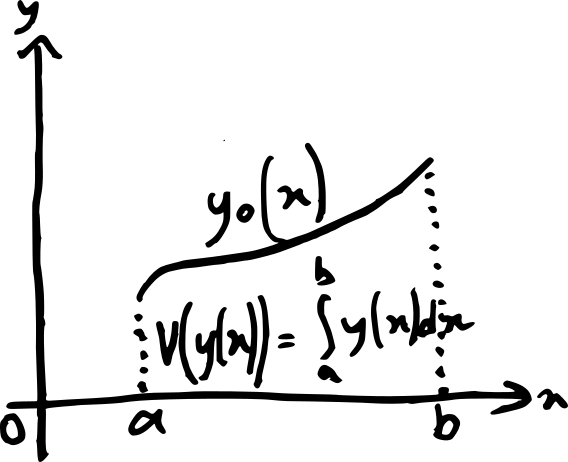
\includegraphics[width=0.9\linewidth]{18} \end{center} \\ \hline
2. \textbf{Приращение независимого аргумента} $\Delta x = x - x_0$, относительно точки $x_0$. &
2. \textbf{Приращение} или \textbf{вариация аргумента} $y(x)$ \textbf{при} $y_0(x)$ функционала $V(y(x))$ называется функция вида $\delta y = y(x) - y_0(x)$, где $y(x)$ произвольно меняется в некотором классе функций. &
\begin{center} 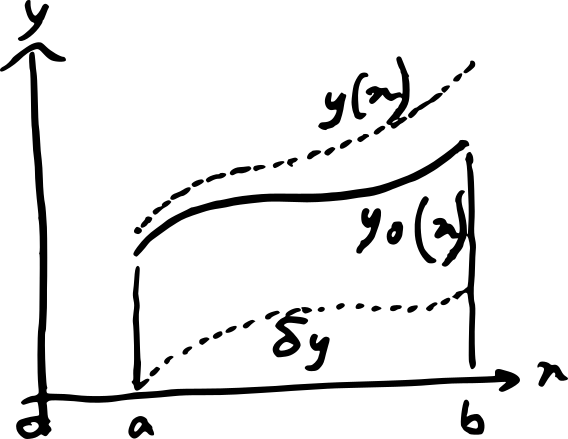
\includegraphics[width=0.9\linewidth]{19} \end{center} \\ \hline
3. Функция $y=f(x)$ \textbf{непрерывна в точке} $x_0$, если $\forall \varepsilon > 0 \quad \exists \delta (\varepsilon):$ \[|x-x_0|<\delta(\varepsilon) \Rightarrow \] \[\Rightarrow |f(x)-f(x_0)|<\varepsilon \] &
3. Функционал \textbf{непрерывен при} $y_0(x)$ в смысле \textbf{близости} $k$-\textbf{го порядка}, если $\forall \varepsilon > 0 \quad \exists \delta (\varepsilon):$ \[V(y(x)) - V(y_0(x))<\varepsilon \textrm{ при:} \] \[\begin{cases} |y(x)-y_0(x)|<\delta(\varepsilon) \\ |y'(x)-y'_0(x)|<\delta(\varepsilon) \\ \cdots \\ |y^{(k)}(x)-y^{(k)}_0(x)|<\delta(\varepsilon) \end{cases} \] \[\forall x \in [a, b] \] &
\begin{center} 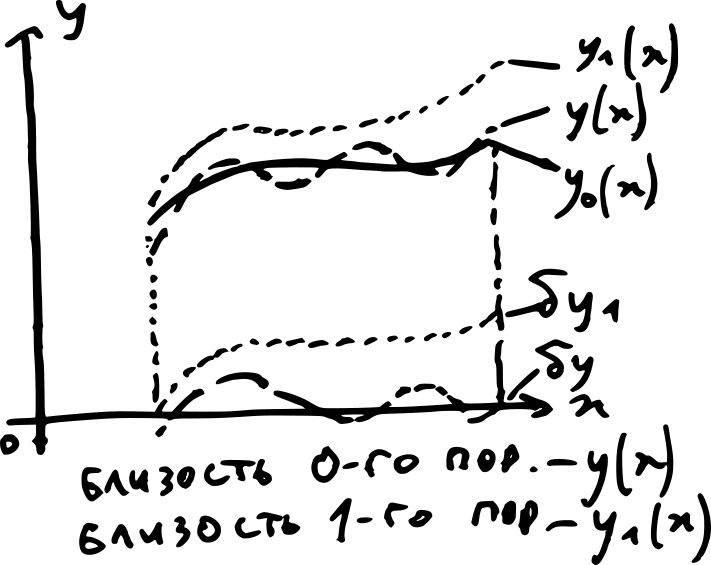
\includegraphics[width=0.9\linewidth]{20} \end{center} \\ \hline
4. \textbf{Линейной функцией} называется функция, удовлетворяющая условиям:
\begin{itemize}
 \item $L(\mathrm{c} x) = \mathrm{c} L(x)$;
 \item $L(x_1 + x_2) = L(x_1) + L(x_2)$.
\end{itemize} &
4. \textbf{Линейным функционалом} $L(y(x))$ называется такой функционал, что:
\begin{itemize}
 \item $L(\mathrm{c} y(x)) = \mathrm{c} L(y(x))$;
 \item $L(y_1(x) + y_2(x)) = L(y_1(x)) + L(y_2(x))$.
\end{itemize} &
Площадь подграфика -- линейный функционал: \[V(y(x)) = \int \limits_a^b y(x) \di x \] \\ \hline
5. \textbf{Приращением функции в точке} $x$ называется функция вида $\Delta f = f(x+\Delta x) - f(x)$. &
5. \textbf{Приращением функционала} $V(y(x))$ \textbf{в точке} $y(x)$ называется функционал от $\delta y$: \[\Delta V = V(y(x) + \delta y) - V(y(x)) \] &
Приращение равно: \begin{tiny} \[\Delta V(y(x)) = \int \limits_a^b (y(x) + \delta y) \di x - \] \[- \int \limits_a^b y(x) \di x = \int \limits_a^b \delta y \di x \] \end{tiny} \\ \hline
6. \textbf{Дифференциалом функции} $y=f(x)$ \textbf{в точке} $x$, если $f(x)$ дифференцируема в точке $x$, называется линейная часть приращения функции, равная $\Delta f = \mathrm{A} \Delta x + o(\Delta x)$, при $\Delta x \to 0$, равная $\di f = \mathrm{A} \Delta x = f_x' \Delta x$. &
6. \textbf{Вариацией функционала} называется линейная часть приращения функционала, то есть линейный относительно $\delta y$ функционал $L(y(x), \delta y)$, такой что $\Delta V = L(y(x), \delta y) + o(\max |\delta y|)$, при $\max |\delta y| \to 0$. &
Здесь в силу линейности функционала его вариация совпадает с приращением: \[\delta V(y(x)) = \int \limits_a^b \delta y \di x = \] \[= \Delta V \] \\ \hline
\end{tabular}
\end{center}
\end{footnotesize}

\newpage\restoregeometry

\textbf{Замечания:}
\begin{enumerate}
 \item Таким образом непрерывность функционала в смысле близости 0-го порядка означает, что максимум приращения функционала не превосходит заданного $\varepsilon$ для всех функций с вариацией $\delta y$, ограниченной $\delta(\varepsilon)$, а близость 1-го порядка означает, что максимум приращения функционала не превосходит заданного $\varepsilon$ для функций, для которых величиной $\delta(\varepsilon)$ ограничена не только её вариация, но и $\delta y'$, вариация её первой производной.\
 \item Вариация функционала в смысле данного выше определения существует не для всякого функционала.
\end{enumerate}

\textbf{Пример:} Рассмотрим функционал $V(y(x)) = \pi \int \limits_a^b y^2 (x) \di x$, равный объёму тела, полученного вращением относительно оси $Ox$ подграфика \textit{непрерывной} функции $y(x)$. Функционал нелинейный. Тогда приращение функционала будет равно:
\[\Delta V(y(x)) = \pi \int \limits_a^b (y(x) + \delta y)^2 \di x - \pi \int \limits_a^b y^2(x) \di x = \pi \int \limits_a^b \left[ 2y(x) \delta y + (\delta y)^2 \right] \di x \]
А его вариация для фиксированной $y(x)$ будет равна $\delta V(y(x)) = 2\pi \int \limits_a^b y(x) \delta y \di x$, так как:
\[\pi \int \limits_a^b (\delta y)^2 = \{ \textrm{по теореме о среднем} \} = (b-a)(\delta y(x_0))^2 = o(\max |\delta y|) \]

\subsubsection{Другое определение дифференциала функции и вариации функционала}

Существует другое, более широкое определение дифференциала функциии вариации функционала.

Если ввести параметр $\alpha \in [0, 1]$, то функция $f(x + \alpha \Delta x)$ при $\alpha = 0$ равна $f(x)$, а при $\alpha = 1$ равна $f(x + \Delta x)$. Частная производная по $\alpha$ при $\alpha = 0$ будет равна дифференциалу в точке $x$:
\[\left. \frac{\partial f(x + \alpha \Delta x)}{\partial \alpha} \right|_{\alpha = 0} = \left. \frac{\di f(x + \alpha \Delta x)}{\di x} \cdot \frac{x + \alpha \Delta x}{\partial \alpha} \right|_{\alpha = 0} = \left. \frac{\di f(x+ \alpha \Delta x)}{\di x} \right| \Delta x = \frac{\di f(x)}{\di x} \Delta x = \di f \]

Таким же образом для функции $n$ переменных можно ввести дифференциал, как производную по $\alpha$ от функции $f(x_1 + \alpha \Delta x_1, \cdots, x_n + \alpha \Delta x_n)$, равную при $\alpha = 0$ её дифференциалу:
\[\frac{\partial f(x_1 + \alpha \Delta x_1, \cdots, x_n + \alpha \Delta x_n)}{\partial \alpha} = \sum_{k=1}^n \frac{\partial f}{\partial x_k} \Delta x_k = \di f \]

Аналогично, для функционала можно ввести вариацию как производную по $\alpha$ от функционала $V(y(x) + \alpha \delta y)$ при $\alpha = 0$, то есть:
\[\delta V = \left. \frac{\partial V(y(x) + \alpha \delta y)}{\partial \alpha} \right|_{\alpha = 0} \]
Покажем, что это совпадает с определением вариации функционала как линейной части приращения, если она существует:
\[\Delta V = V(y(x) + \delta y) - V(y(x)) = L(y(x), \delta y) + o(\max |\delta y|), \quad \textrm{при} \quad \max |\delta y| \to 0 \]
Тогда производная от $V(y(x) + \alpha \delta y)$ по $\alpha$ будет равна:
\[\left. \frac{\partial V(y(x) + \alpha \delta y)}{\partial \alpha} \right|_{\alpha = 0} = \left. \lim_{\Delta \alpha \to 0} \frac{\Delta V}{\Delta \alpha} \right|_{\alpha = 0} = \lim_{\alpha \to 0} \frac{\Delta V}{\alpha} = \lim_{\alpha \to 0} \frac{V(y(x) + \alpha \delta y) - V(y(x))}{\alpha} = \]
\[= \lim_{\alpha \to 0} \frac{L(y(x) + \alpha \delta y) + o(\alpha \delta y)}{\alpha} = \lim_{\alpha \to 0} \frac{L(y(x) + \alpha \delta y)}{\alpha} + \lim_{\alpha \to 0} \frac{o(\alpha \delta y)}{\alpha} = \]
\[= \lim_{\alpha \to 0} \frac{\alpha L(y(x) + \delta y)}{\alpha} + \lim_{\alpha \to 0} \frac{o(\alpha \delta y)}{\alpha} = L(y(x) + \delta y) + 0 = L(y(x) + \delta y) = \delta V \]

\textbf{Пример:} Вычислим вариацию функционала $V(y(x)) = \pi \int \limits_a^b y^2(x) \di x$.
\[\delta V(y(x)) = \left. \frac{\partial V(y(x) + \alpha \delta y)}{\partial \alpha} \right|_{\alpha = 0} = \left. \frac{\partial}{\partial \alpha} \pi \int \limits_a^b (y(x) + \alpha \delta y)^2 \di x \right|_{\alpha = 0} = \]
\[= \left. \frac{\partial}{\partial \alpha} \pi \int \limits_a^b (y^2 + 2y(x)\alpha \delta y + \alpha^2 (\delta y)^2) \di x \right|_{\alpha = 0} = \left. \pi \int \limits_a^b (2y(x) \delta y + 2\alpha (\delta y)^2) \di x \right|_{\alpha = 0} = \pi \int \limits_a^b 2y(x) \delta y \di x \]

\subsubsection[Вариация интегрального функционала вида $\int \limits_a^b F(x, y(x), y'(x)) \di x$]{Вариация интегрального функционала вида $V(y(x)) = \int \limits_a^b F(x, y(x), y'(x)) \di x$}

Используя второе определение вариации и правило дифференцирования интеграла по параметру, а также предполагая существование необходимых производных, имеем:
\[\left. \delta V(y(x)) = \frac{\partial V(y(x) + \alpha \delta y)}{\partial \alpha} \right|_{\alpha = 0} = \left. \frac{\partial}{\partial \alpha} \int \limits_a^b F(x, y(x) + \alpha \delta y, y'(x) + \alpha (\delta y')) \di x \right|_{\alpha = 0} = \]
\[= \left. \int \limits_a^b \left( F_y'(x, y(x) + \alpha \delta y, y'(x) + \alpha (\delta y')) \cdot \delta y + F_{y'}'(x, y(x) + \alpha \delta y, y'(x) + \alpha (\delta y')) \cdot (\delta y') \right) \di x \right|_{\alpha = 0} = \]
\[= \left. \int \limits_a^b \left( F_y'(x, y(x), y'(x)) \cdot \delta y + F_{y'}' (x, y(x), y'(x)) \cdot (\delta y') \right) \di x \right|_{\alpha = 0} = \int \limits_a^b (F_y' \delta y + F_{y'}' (\delta y')) \di x \]
Интегрируя второе слагаемое по частям, учитывая неподвижность границ (то есть вариации $y(x)$ на концах $[a, b]$ равны нулю), упростим выражение:
\[\delta V(y(x)) = \int \limits_a^b (F_y' \delta y + F_{y'}' (\delta y')) \di x = \Bigl\{ (\delta y') = (\delta y)' \Bigr\} = \int \limits_a^b F_y' \delta y \di x + \int \limits_a^b F_{y'}' (\delta y)' \di x = \]
\[= \int \limits_a^b F_y' \delta y \di x + \Bigl. F_{y'}' \delta y \Bigr|_{x=a}^{x=b} - \int \limits_a^b \frac{\di}{\di x} (F_{y'}') \delta y \di x = \Bigl\{ \delta y(a) = \delta y(b) = 0 \Bigr\} = \int \limits_a^b \left( F_y' - \frac{\di}{\di x} (F_{y'}') \right) \delta y \di x \]

В общем, формулу для вариации интегрального функционала, заданного на классе функций $C^1[a, b]$, можно записать в виде: $\delta V(y(x)) = \int \limits_a^b \left( F_y' - \frac{\di}{\di x} (F_{y'}') \right) \delta y \di x$.

\subsection{Экстремумы интегральных функционалов с постоянными границами}

Основные задачи вариационного исчисления - это поиск оптимальных решений, то есть функций, которые реализуют минимум или максимум какой-то целевой функции (и часто выражаются через интегралы). Мы рассмотрим простейшие задачи - экстремумы интегральных функционалов с неподвижными границами.

\subsubsection{Определение экстремума функционала}

Как известно, для функций одного переменного существует две постановки задач на экстремум: отыскание локального экстремума и отыскание глобального экстремума на множестве, то есть экстремум в локальной окрестности или наибольшее и наименьшее значение на множестве. Таким образом вводятся понятие \textit{сильного экстремума}.

\textbf{Экстремум} (максимум или минимум) \textbf{функционала} $V(y(x))$ \textbf{достигается на функции} $y_0(x)$, если он принимает наибольшее (наименьшее) среди всех значений функционала на множестве функций $D$ из определённого значения, то есть функция $y_0(x)$ реализует $\max$ ($\min$) $V(y(x))$ на $D$($[a,b]$), если:
\[\forall y(x) \in D([a, b]) \quad \Rightarrow \quad V(y(x)) \leq V(y_0(x)), \quad (V(y(x)) \geq V(y_0(x))) \]
Если неравенство строгое, то \textbf{экстремум} называется \textbf{строгим}.

\textbf{Экстремум} (максимум или минимум) \textbf{функционала} $V(y(x))$ называется \textbf{сильным}, если он достигается на \textit{функции нулевого порядка близости}, то есть:
\[\forall y(x) \in D([a, b]): \quad |\delta y| = |y(x) - y_0(x)| < \varepsilon \quad \Rightarrow \]
\[\Rightarrow \quad V(y(x)) > V(y_0(x)), \quad (V(y(x)) < V(y_0(x))) \]

\textbf{Экстремум} (максимум или минимум) \textbf{функционала} $V(y(x))$ называется \textbf{слабым}, если он достигается на \textit{функции первого порядка близости}, то есть:
\[\forall y(x) \in D([a, b]): \quad \begin{cases} |\delta y| = |y(x) - y_0(x)| < \varepsilon \\ |\delta y'| = |y'(x) - y_0'(x)| < \varepsilon \end{cases} \quad \Rightarrow\]
\[\Rightarrow \quad V(y(x)) > V(y_0(x)), \quad (V(y(x)) < V(y_0(x))) \]

Так как класс вариаций нулевого класса близости шире, чем класс первого класса близости (см. пункт 4.2.3), поэтому, если реализуется \textit{сильный экстремум}, то автоматически реализуется и \textit{слабый экстремум}.

\subsubsection{Необходимое условие экстремума функционала}

Необходимое условие экстремума для гладкой функции в точке - равенство нулю производной в этой точке. Аналогично, для функционала необходимое условие экстремума - \textit{вариация функционала на функции, реализующей этот экстремум, равна нулю}.

\begin{wrapfigure}[10]{l}{0.25\textwidth}
  \centering
  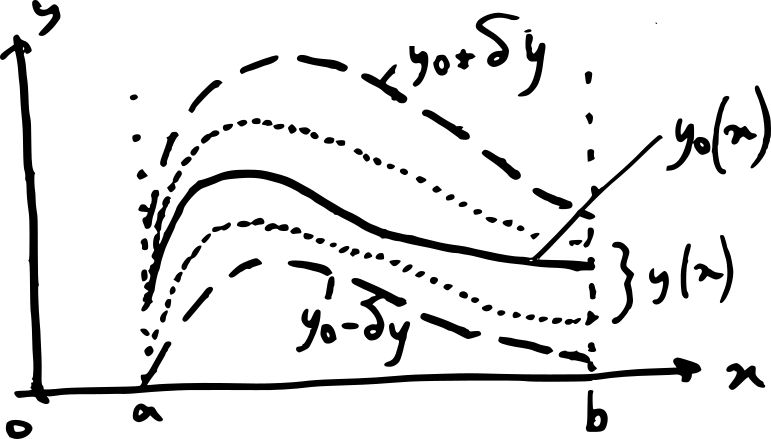
\includegraphics[width=0.25\textwidth]{21}
  \vspace{-4mm}
  \caption{Внутренняя точка области $D([a,b])$}
\end{wrapfigure}

Введём еще одно понятие - \textit{внутренней точки области} множества функций $D([a, b])$.

Функция $y_0(x)$ - \textbf{внутренняя точка области} $D([a, b])$, если все функции $y(x)$ такие, что:
\[y(x) = y_0(x) + \alpha \delta y \in D([a, b]), \quad \forall \alpha \in [-1, 1], \quad \forall \delta y \in D([a, b]) \]

\textbf{Теорема:} Если функционал $V(y(x))$, заданный на области $D([a, b])$, достигает экстремума на функции $y_0(x)$, которая есть внутренняя точка области $D$, то вариация функционала $V(y(x))$ на функции $y_0(x)$ равна нулю, то есть $\delta V(y_0(x)) = 0$.

\textbf{Док-во:} При фиксированных функциях $y_0(x)$ и $\delta y$ функционал $V(y(x)) = V(y_0(x) + \alpha \delta y) = \varphi (\alpha)$ есть функция от $\alpha$, $\forall \alpha \in [-1, 1]$, которая по условию теоремы достигает при $\alpha = 0$ своего экстремума, следовательно, производная $\varphi^{\prime}(0) = 0$. А из второго определения вариации:
\[\varphi^{\prime}(0) = \Bigl. \varphi^{\prime}(\alpha) \Bigr|_{\alpha = 0} = \left. \frac{\partial V(y(x) + \alpha \delta y)}{\partial \alpha} \right|_{\alpha = 0} \defeq \delta V = 0 \]

\textbf{Замечания:}
\begin{enumerate}
 \item Если на кривой $y_0(x)$ достигается экстремум функционала $V(y(x))$, то для любого семейства функций $y(x, \alpha)$ такого, что $y(x, 0) = y_0(x)$, а $y(x, 1) = y_0(x) + \delta y$, следует, что $\left. \frac{\partial V(y(x, \alpha))}{\partial \alpha} \right|_{\alpha = 0} = 0$.
 
 Эта производная, вообще говоря, может и не совпадать с вариацией функционала, но обращается в ноль вместе с вариацией функционала $\delta V(y_0(x))$ на реализующих экстремум функциях. 
 \item Аналогично можно перенести все понятия и результаты на функционалы от нескольких функций $V(y_1(x), y_2(x), \cdots, y_n(x))$ или от функции нескольких переменных \\ $V(y(x_1, x_2, \cdots, x_n))$.
\end{enumerate}

\subsubsection{Основная лемма вариационного исчисления}

\textbf{Теорема:} Если для любой непрерывной функции $\varphi (x)$ на интервале $[a, b]$ имеем
\[\int \limits_a^b f(x) \varphi (x) \di x = 0,\]
где $f(x)$ непрерывна на $[a, b]$, то $f(x) \equiv 0$ на $[a, b]$.

\textbf{Док-во} (от противного)\textbf{:} Предположим, что $f(x) \not = 0$ на $[a, b]$, следовательно:
\[\exists x_0 \in [a, b]: \quad f(x_0) \not = 0 \]
Положим для определённости, что $f(x) > 0$. Тогда по теореме о стабилизации знака $\exists U(x_0) \not = \varnothing$, такая, что $f(x)>0, \quad \forall x \in U(x_0)$.

\begin{wrapfigure}{l}{0.25\textwidth}
  \centering
  \vspace{-5mm}
  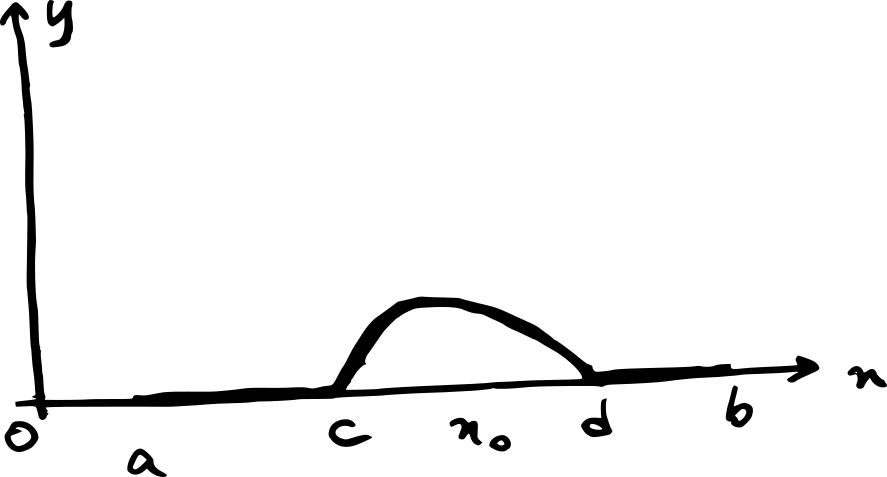
\includegraphics[width=0.25\textwidth]{22}
  \vspace{-8mm}
  \caption{Подобранная функция}
\end{wrapfigure}

Если подобрать функцию $\varphi (x)$, равную нулю всюду кроме интервала $[c, d] \not = \varnothing \subset U(x_0)$, например, $\varphi (x) = (x-c)^{2k}(x-d)^{2m}$, тогда $f(x) \cdot \varphi(x) > 0, \quad \forall x \in [c, d]$. Тогда:
\[\int \limits_a^b f(x) \varphi (x) \di x = \int \limits_c^d f(x) \varphi (x) \di x > 0 \]
Это противоречит условию теоремы, следовательно, предположение неверно, и $f(x) \equiv 0$ на $[a, b]$.

\subsubsection[Уравнение Эйлера для простейших вариационных задач]{Уравнение Эйлера для простейших вариационных задач -- функционалов вида $V(y(x)) = \int \limits_a^b F(x, y, y') \di x$}

Уравнение Эйлера позволяет свести необходимое условие экстремума -- равенство нулю вариации функционала $\delta V(y(x)) = 0$ к более простому условию, выраженному дифференциальным уравнением.

Действительно, вариация функционала равна следующему (см. пункт 4.2.6):
\[\delta V(y(x)) = \int \limits_a^b \left( F_y' - \frac{\di}{\di x} (F_{y'}') \right) \delta y \di x \]
Необходимое условие экстремума $\delta V(y(x)) = \int \limits_a^b \left( F_y' - \frac{\di}{\di x} (F_{y'}') \right) \delta y \di x = 0$, для любой вариации $\delta y$. Тогда из основной леммы вариационного исчисления (см. пункт 4.3.3) следует, что
\[\delta V(y(x)) = 0 \quad \Leftrightarrow \quad \left( F_y' - \frac{\di}{\di x} (F_{y'}') \right) = 0 \]

При условии, что $F(x, y, y')$ дважды непрерывно дифференцируемая функция по всем трём переменным, тогда по правилу дифференцирования сложной функции имеем:
\[\left( F_y' - \frac{\di}{\di x} (F_{y'}' (x, y, y')) \right) = F_y' - F_{xy'}^{\prime \prime} - F_{yy'}^{\prime \prime} y' - F_{y'y'}^{\prime \prime} y^{\prime \prime} \]

Откуда получаем \textbf{дифференциальное уравнение Эйлера} (1744 год):
\[F_y' - F_{xy'}^{\prime \prime} - F_{yy'}^{\prime \prime} y' - F_{y'y'}^{\prime \prime} y^{\prime \prime} = 0 \]

Это обыкновенное дифференциальное уравнение второго порядка относительно неизвестной функции $y(x)$. Решения уравнения Эйлера называются \textbf{экстремалями}. Только на них возможен экстремум функционала. Чтобы найти кривую, реализующую экстремум, находим ту, которая удовлетворяет граничным условиям: $y(a)=y_1$, $y(b)=y_2$.

\textbf{Замечание:} Эта задача не всегда имеет решение, а когда имеет, оно может быть не единственным. Но важно и то, что даже в случае нахождения решения краевой задачи, оно может не быть решением вариационной задачи, так как удовлетворено только необходимое, но не достаточное условие. Следовательно, требуется проверка, будет ли экстремаль решением вариационной задачи.

\subsubsection{Частные случаи интегрирования уравнения Эйлера}

В следующих случаях можно получить решения уравнения Эйлера. В общем случае нет универсального алгоритма.
\begin{enumerate}
 \item $F(x, y, y') = F(x, y)$, то есть не зависит явно от $y'$. Уравнение Эйлера примет вид $\frac{\partial}{\partial y}  F(x, y) = 0$. Если вид функции $F(x, y)$ известен, то и $F_y'(x, y)$ -- тоже известная функция, определяющая кривую $F_y'(x, y) = 0$, которая может и не проходить через граничные точки $(a, y_1)$ и $(b, y_2)$. Но если проходит, то это будет решением задачи.
 \item $F(x, y, y') = M(x, y) + N(x, y) \cdot y'$ -- линейная функция от $y'$. Тогда уравнение Эйлера после дифференцирования примет вид:
 \[\frac{\partial F}{\partial y} = \frac{\partial M}{\partial y} + \frac{\partial N}{\partial y} y', \quad \frac{\partial F}{\partial y'} = N, \quad \frac{\di}{\di x} \frac{\partial F}{\partial y'} = \frac{\di N}{\di x} = \frac{\partial N}{\partial x} + \frac{\partial N}{\partial y} y' \quad \Rightarrow \quad \frac{\partial M}{\partial y} - \frac{\partial N}{\partial x} = 0 \]
 Получено конечное уравнение при произвольных $M(x, y)$ и $N(x, y)$. Если оно выполняется тождественно, то получили условие существования потенциала $U(x,y)$ для векторного поля:
 \[F = \grad U = M(x, y) \vec{i} + N(x, y) \vec{j} \]
 Таким образом интегрирование уравнения Эйлера сведётся к известной задаче восстановления скалярного потенциала по его градиенту. И значение интеграла, то есть функционала, не зависит от пути интегрирования, то есть не зависит от кривой $y(x)$.
 \item $F(x, y, y') = F(y')$ -- зависит только от $y'$. После подстановки в уравнение Эйлера получаем:
 \[\frac{\di}{\di x} \frac{\partial F}{\partial y'} = F_{y'y'}^{\prime \prime} y^{\prime \prime} = 0 \quad \Leftrightarrow \quad \begin{sqcases} F_{y'y'}^{\prime \prime} = 0 \\ y^{\prime \prime} = 0 \end{sqcases} \quad \Leftrightarrow \quad \begin{sqcases} F = k_1y' + k_2 \\ y = c_1x + c_2 \end{sqcases} \]
 То есть экстремалями являются прямые $y = c_1x + c_2, \quad c_1, c_2 \in \mathbb{R}$. Осталось подобрать по граничным условиям $c_1$ и $c_2$.
 \item $F(x, y, y') = F(x, y')$ -- не зависит явно от $y$. Тогда уравнение Эйлера принимает вид:
 \[\frac{\di}{\di x} \frac{\partial F}{\partial y'} = 0 \quad \Leftrightarrow \quad \frac{\partial F(x, y')}{\partial y'} = c_1 \quad \Leftrightarrow \quad y' = f(x, c_1) \quad \Rightarrow \quad y(x) = \int f(x, c_1) \di x + c_2 \]
 \item $F(x, y, y') = F(y, y')$ -- не зависит явно от $x$. После подстановки в уравнение Эйлера получим:
 \[\frac{\partial F(y, y')}{\partial y} - \frac{\di}{\di x} \frac{\partial F(y, y')}{\partial y'} = 0 \quad \Leftrightarrow \quad F_y' - F_{y'y'}^{\prime \prime}y^{\prime \prime} - F_{y'y}^{\prime \prime}y' = 0 \quad \Leftrightarrow \]
 \[\Leftrightarrow \quad (F_y' - F_{y'y'}^{\prime \prime}y^{\prime \prime} - F_{y'y}^{\prime \prime}y')y' = 0 = \]
 \[= \left\{ \frac{\di}{\di x} (F - y'F_{y'}') = F_y'y' + \underbrace{F_{y'}'y^{\prime \prime} - y^{\prime \prime}F_{y'}'}_0 - y'F_{y'y'}^{\prime \prime}y^{\prime \prime} - y'F_{y'y}^{\prime \prime}y' \right\} = \]
 \[= \frac{\di}{\di x} (F - y'F_{y'}') = 0 \quad \Leftrightarrow \quad F - y'F_{y'}' = c \quad \Leftrightarrow \quad y' = \varphi (y) \]
 Получаем уравнение с разделяющимися переменными. Если не удается разрешить, то применяется метод введения параметра, применяемый, например, при интегрировании уравнений Лагранжа и Клеро.
\end{enumerate}

\newpage

Подытожим все разобранные случаи в виде краткой таблицы:

\begin{small}
\begin{center}
\begin{tabular}{|p{4mm}|p{4cm}|p{50mm}|p{56mm}|}
\hline
№ & \textbf{Вид функции} \newline $F(x, y, y')$ & \textbf{Вид уравнения Эйлера} \newline \[\frac{\partial F}{\partial y} - \frac{\di}{\di x} \frac{\partial F}{\partial y'} = 0 \] & \textbf{Решения уравнения} \newline \textbf{Эйлера} \\ \hline
1 & $F(x, y, y') = F(x, y)$ \newline не зависит от $y'$. & \[\frac{\partial}{\partial y} F(x, y) = 0 \] & Так как вид функции $F(x, y)$ известен, то уравнение \newline $F_y(x, y) = 0$ определяет конкретные кривые на плоскости, которые могут и не проходить через граничные точки $(a, y_1)$ и $(b, y_2)$. \\ \hline
2 & $F(x, y, y') =$ \newline $= M(x, y) + N(x, y) y'$ \newline линейно зависит от $y'$. & \[\frac{\partial F}{\partial y} = \frac{\partial M}{\partial y} + \frac{\partial N}{\partial y} y' \] \[\frac{\partial F}{\partial y'} = N \] \[\frac{\di}{\di x} \frac{\partial F}{\partial y'} = \frac{\di N}{\di x} = \frac{\partial N}{\partial x} + \frac{\partial N}{\partial y} y' \] \[\frac{\partial M}{\partial y} - \frac{\partial N}{\partial x} = 0 \] & Если полученное конечное уравнение выполняется тождественно, то существует потенциальная функции $U(x, y)$. Значения функционала не зависит от пути интегрирования. Нужно проверить соблюдение граничных условий $(a, y_1)$ и $(b, y_2)$. \\ \hline
3 & $F(x, y, y') = F(y')$ \newline зависит только от $y'$. & \[\frac{\di}{\di x} \frac{\partial F}{\partial y'} = F_{y'y'}^{\prime \prime} y^{\prime \prime} = 0 \] & Экстремали: $y = c_1x + c_2$. \\ \hline
4 & $F(x, y, y') = F(x, y')$ \newline не зависит от $y$. & \[\frac{\di}{\di x} \frac{\partial F}{\partial y'} = 0 \] \[\frac{\partial F(x, y')}{\partial y'} = c \] & Экстремали -- решения ОДУ-1, получающегося после разрешения относительно $y'$ уравнения $F_{y'}'(x, y') = c$ или методом введения параметра. \\ \hline
5 & $F(x, y, y') = F(y, y')$ \newline не зависит от $x$. & \[\frac{\partial F(y, y')}{\partial y} - \frac{\di}{\di x} \frac{\partial F(y, y')}{\partial y'} = 0 \] \[F_y' - F_{y'y'}^{\prime \prime}y^{\prime \prime} - F_{y'y}^{\prime \prime}y' = 0 \] \[(F_y' - F_{y'y'}^{\prime \prime}y^{\prime \prime} - F_{y'y}^{\prime \prime}y')y' = 0 \] \[\frac{\di}{\di x} (F - y'F_{y'}') = 0 \] \[F - y'F_{y'}' = c \] \[y' = \varphi (y) \] & Разрешая уравнение относительно $y'$, получим ОДУ-1 вида $y' = f(y)$, то есть уравнение с разделяющимися переменными. Если не удаётся разрешить, то поможет метод введения параметра. \\ \hline
\end{tabular}
\end{center}
\end{small}

\newpage

\subsubsection{Примеры решения случаев интегрирования уравнения Эйлера}

\begin{enumerate}
 \item $V(y(x)) = \int \limits_a^b y^2 \di x, \quad y(a) = y_1, \quad y(b) = y_2$. Уравнение Эйлера примет вид:
 \[\frac{\partial F}{\partial y} - \frac{\di}{\di x} \frac{\partial F}{\partial y'} = 0 \quad \Leftrightarrow \quad 2y = 0 \quad \Leftrightarrow \quad y = 0 \]
 Тогда при $y_1 = y_2 = 0$ это будет экстремаль, в прочих случаях в классе непрерывных функций решений нет. Минимум функционала будет достигаться на разрывной функции:
 \[y(x) = \begin{cases} y_1, & x=a \\ 0, & x \in (a, b) \\ y_2, & x=b \\ \end{cases} \]
 \item $V(y(x)) = \int \limits_a^b (y^2 + x^2y') \di x, \quad y(a) = y_1, \quad y(b) = y_2$. Уравнение Эйлера примет вид:
 \[2y - 2x = 0 \quad \Leftrightarrow \quad y = x \]
 Если условия выполняются, то прямая $y = x$ -- экстремаль.
 \item $V(y(x)) = \int \limits_a^b \sqrt{1 + y^{\prime 2}} \di x, \quad y(a) = y_1, \quad y(b) = y_2$ -- длина дуги кривой, проходящей через фиксированные точки. Экстремали: $y = c_1x + c_2$, константы определяются из граничных условий, в итоге получим:
 \[y = \frac{y_2-y_1}{b-a} (x-a) + y_1 \]
 \item $V(y(x)) = \int \limits_a^b \frac{\sqrt{1 + y^{\prime 2}}}{x} \di x, \quad y(a) = y_1, \quad y(b) = y_2$. Уравнение Эйлера примет вид:
 \[\frac{\di}{\di x} \frac{\partial}{\partial y'} \frac{\sqrt{1 + y^{\prime 2}}}{x} = 0 \quad \Leftrightarrow \quad \frac{y'}{x \sqrt{1 + y^{\prime 2}}} = c_1 \]
 Интегрируем методом введения параметра $y' = \tg t$:
 \[\frac{\di y}{\di x} = \frac{y_t'}{x_t'} = \frac{c_1y_t'}{\cos t} = \tg t \quad \Leftrightarrow \quad y_t' = \frac{1}{c_1} \tg t \cos t = \frac{1}{c_1} \sin t \quad \Leftrightarrow \quad y = -\frac{1}{c_1} \cos t + c_2 \]
 Исключив параметр $t$, получим:
 \[x^2 + (y-c_2)^2 = \frac{1}{c_1^2} \]
 \item В качестве примера задача о наименьшей площади поверхности вращения: определить кривую с заданными граничными точками, при вращении которой вокруг оси $Ox$ образуется поверхность наименьшей площади.
 \[V(y(x)) = S(y(x)) = 2\pi \int \limits_a^b y \sqrt{1 + y^{\prime 2}} \di x, \quad y(a) = y_1, \quad y(b) = y_2 \]
 Уравнение Эйлера $F - y' \frac{\partial F}{\partial y'} = c_1$ примет вид:
 \[y \sqrt{1 + y^{\prime 2}} - \frac{yy^{\prime 2}}{\sqrt{1 + y^{\prime 2}}} = c_1 \quad \Leftrightarrow \quad \frac{y}{\sqrt{1 + y^{\prime 2}}} = c_1 \]
 Интегрируем методом введения параметра $y' = \sh t$. Тогда из уравнения получим $y = c_1 \ch t$. Используя формулу для производной в параметрической форме $y_x' = \frac{y_t'}{x_t'}$, получим уравнения для $x$ относительно:
 \[x_t' = \frac{y_x'}{y_t'} = \frac{c_1 \sh t}{\sh t} = c_1 \quad \Leftrightarrow \quad x = c_1t + c_2 \]
 Тогда, исключив параметр $t$, получим:
 \[y = c_1 \ch \left( \frac{x-c_2}{c_1} \right) \]
 Это уравнение цепной линии. После подстановки граничных условий получим значения констант. Поверхности, полученные вращением цепной линии, называют \textit{катеноидами}. Стоит отметить, что в зависимости от взаимного расположения граничных точек может быть одно, два или ни одного решения.
\end{enumerate}

\section{Введение в теорию графов}

\subsection{Основные понятия}

\subsubsection{Примеры графов}

Мы встречаемся с графами буквально на каждом шагу: схема метро, блок-схема программы для ЭВМ, генеалогическое древо, схема управления (фирмой, технологическим процессом, воинским подразделением $\cdots$), электросхемы, схема внутримолекулярных связей -- всё это графы. Во всех случаях \textit{сложные объекты} (метро, программы, династии, организации, электроприборы, молекулы) представляются в виде \textit{совокупности однородных элементов} (станций, людей, операторов алгоритмического языка, электронагрузок, атомов), между которыми имеются \textit{однородные связи}, или \textit{отношения} (прямое сообщение между станциями, последовательность выполнения операций, отношения родства, иерархия подчинения, электрические провода, химическая связь). Эти связи могут быть двух типов: \textit{симметричные} и \textit{несимметричные}. Примерами симметричных связей могут служить улицы с двухсторонним движением, связывающие перекрёстки города, электропровода, отношения знакомства, дружбы. Примерами односторонних (несимметричных) связей служат улицы с односторонним движением, отношения подчинённости -- <<руководитель-подчинённый>>, кровного родства -- <<предок-потомок>>.

Теория графов изучает такие структуры независимо от их конкретной природы, то есть способами их математического описания, свойствами, сравнением и так далее. Структуру связей наглядно изображают в виде картинки, состоящей из точек, называемых вершинами, соединенных отрезками (\textit{рёбрами}) (слева) в случае симметричных связей или стрелочками (\textit{дугами}), если связи несимметричные (\textit{посередине}). Возможны смешанные графы (справа), содержащие как рёбра, так и дуги.

\begin{figure}[h]
 \centering
 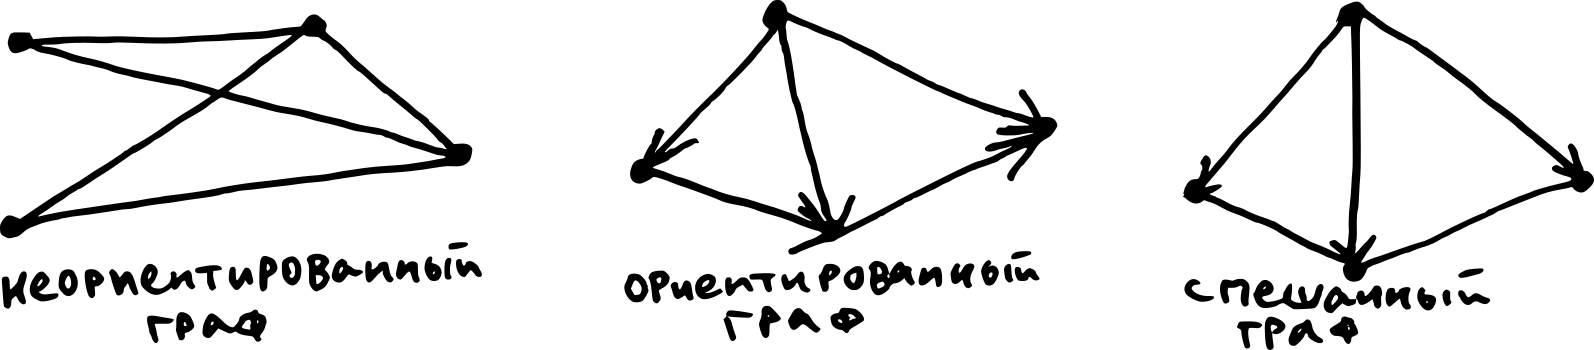
\includegraphics[width=0.7\textwidth]{23}
 \vspace{-4mm}
  \caption{Виды графов}
\end{figure}

\subsubsection{История теории графов и её основные задачи}

Начало развития теории графов относят к 1736 году, когда Леонард Эйлер решил знаменитую задачу о кёнигсбергских мостах: можно ли обойти семь мостов, соединяющих два острова (А, В) и два берега реки (С, D), как показано на \textit{Рис. 22}, так, чтобы пройдя по каждому мосту один раз, вернуться в исходную точку. Отношения пешеходной доступности отображаются графом справа.

\begin{figure}[h]
 \centering
 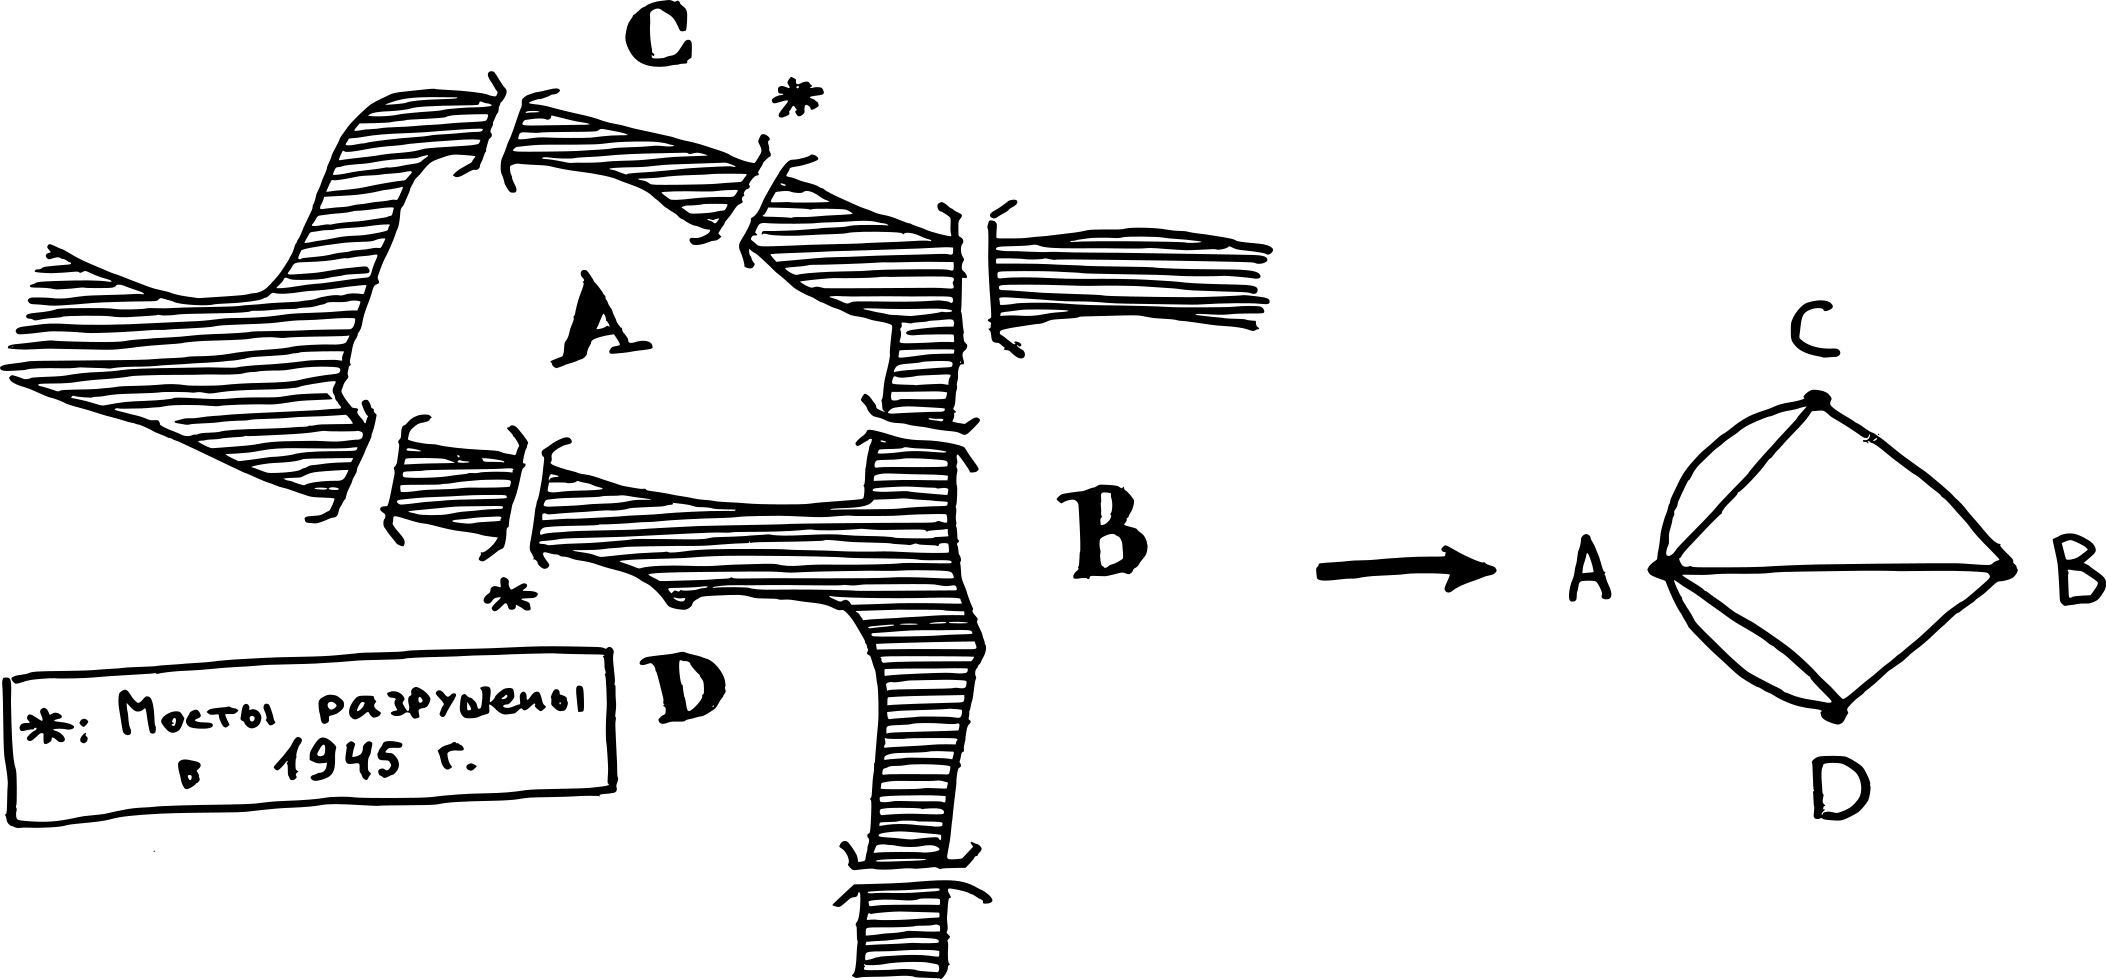
\includegraphics[width=0.7\textwidth]{24}
 \vspace{-4mm}
  \caption{Кёнигсбергские мосты}
\end{figure}

Так Л. Эйлер, прогуливаясь по набережным Кёнигсберга, сформулировал и решил общую проблему, которая в современных терминах звучит так: \textit{при каких условиях связный граф содержит цикл, проходящий через каждое его ребро?}

Почти сто лет это был единственный результат в теории графов. Следующий шаг был сделан инженером-электриком Г. Кирхгофом, разработавшим теорию деревьев для исследования электрических цепей, связанную с задачей минимизации длины проводов к конечному числу точек подключения. А задачи о количестве возможных изомеров в углеводородных цепях привели английского математика А. Кэли к решению перечислительных задач для трех типов деревьев.

Бурное развитие теории графов приходится на вторую половину 20-го века и начало 21-го из-за стремительного роста приложений в области экономики и статистики, химии и биологии. Этим объясняется некоторая неустойчивость в терминологии. В терминах теории графов моделируются огромное число задач, связанных прежде всего с задачами управления дискретными объектами, теории расписаний, теории сетевого планирования, проектирования интегральных микросхем и так далее.

Огромное количество разнообразных по форме задач может быть сведено к основным задачам теории графов: задаче \textit{о кратчайшем маршруте}, задаче \textit{о наибольшем потоке}, задаче \textit{о наименьшем дереве}, задаче \textit{о паросочетаниях}.

\subsubsection{Определение неориентированного графа и его элементов}

Впервые термин <<граф>> появился в книге венгерского математика Д. Кёнига в 1936 году. В технической литературе можно встретить определение графа, восходящее к его наглядной интерпретации, а именно: \textit{графом называется совокупность вершин и связывающих их рёбер} (или \textit{дуг}).

Но это определение недостаточно потому, что его можно трактовать неоднозначно, трудно изобразить пространственный граф (например, модель кристаллической решетки) на плоскости, трудно стандартизировать различные графы. Посмотрим на два изображения одного того же графа.

\begin{figure}[h]
 \centering
 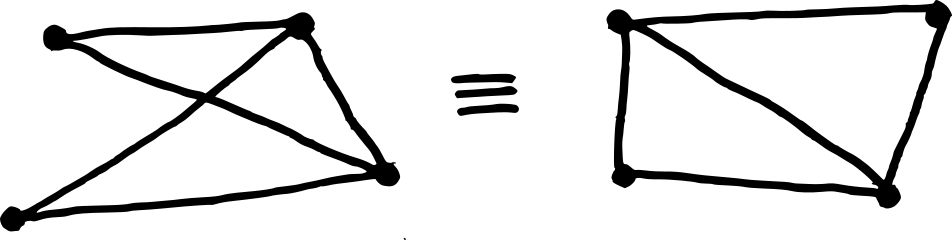
\includegraphics[width=0.4\textwidth]{25}
 \vspace{-4mm}
  \caption{Эквивалентные графы}
\end{figure}
Ниже приведены строгие теоретико-множественные определения.

Пусть $V$ -- непустое конечное множество, $V^{(2)}$ -- множество его двухэлементных подмножеств. Тогда:
\begin{enumerate}
 \item упорядоченная пара $(V, E)$, где $E$ -- произвольное подмножество множества $V^{(2)}$, называется \textbf{неориентированным графом};
 \item элементы множества $V$ называются \textbf{вершинами графа};
 \item элементы множества $E$ называются \textbf{рёбрами графа};
 \item \textbf{порядком графа} называется число его вершин.
\end{enumerate}
\textbf{Обозначения:} Пусть имеется граф $G$, тогда:
\begin{itemize}
 \item $V(G) = \{ 1, 2, \cdots, n \}$ -- множество вершин;
 \item $|V(G)| = n$ -- количество вершин, порядок графа;
 \item $E(G)$ -- множество рёбер графа;
 \item $|E(G)| = m$ -- число рёбер графа;
 \item $(i,j)=(j,i)$ -- ребро, соединяющее вершины $i,j \in V$.
\end{itemize}

Если у графа $G$ имеем $|V(G)| = n$, а $|E(G)| = m$, то этот граф называется $(n, m)$-\textbf{графом}. Таким образом, граф $G = E(G) \cup V(G)$ -- совокупность $n$ вершин и $m$ рёбер.

\textbf{Замечание:} В технической литературе рёбра обозначаются через вершины, которые они связывают, например, $(1, 2)$. Иногда их обозначают буквами с индексом $e_i, \quad i=\bar{1,m}$.

Граф $G$ называется \textbf{пустым} (\textbf{ноль-графом}), если множество его рёбер пусто, то есть $|E(G)| = 0$. Фактически, он представляет из себя \textit{совокупность} $n$ \textit{несвязанных вершин} и обозначается $O_n$.

\begin{wrapfigure}{r}{0.25\textwidth}
  \centering
  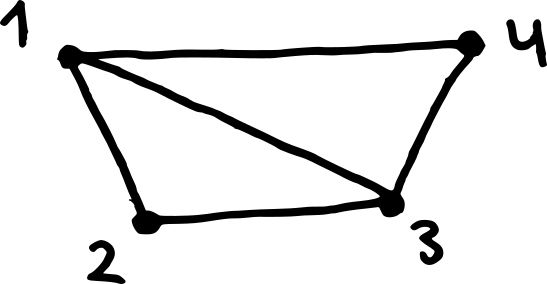
\includegraphics[width=0.25\textwidth]{26}
  \vspace{-4mm}
  \caption{Помеченный граф $G$}
\end{wrapfigure}

Граф $G$ называется \textbf{помеченным графом}, если его вершины помечены индивидуальным символом, чаще всего числами или буквами.

\textbf{Пример:} Отметим числами от 1 до 4 вершины графа $G$ на \textit{Рис. 24}. Граф $G$ -- это $(4,5)$-граф, его порядок $|V(G)| = 4$, число рёбер $|E(G)| = 5$, множество вершин $V(G) = \{ 1, 2, 3, 4 \}$, множество рёбер
\[E(G) = \{ (1,2),(1,3),(1,4),(2,3),(3,4) \}. \]

\subsubsection{Отношения смежности и инцидентности для неориентированного графа}

Между вершинами существует \textit{отношение смежности}, и между рёбрами графа существует \textit{отношение смежности}, а между вершинами и рёбрами -- \textit{отношение инцидентности}. Эти отношения помогают описать графы универсальным образом с помощью \textit{матриц смежности и инцидентности}.

\textbf{Смежными вершинами} графа $G$ называются вершины $u$ и $v$, для которых ребро $(u,v) \in E(G)$, то есть вершины $u,v$ соединены ребром из множества $E$ (рёбер графа $G$), в противном случае они \textbf{несмежные}.

\textbf{Смежными рёбрами} графа $G$ называются рёбра $(u,v) \in E$, то есть рёбра графа, имеющие общую концевую вершину.

\textbf{Вершина} $v$ и \textbf{ребро} $(i,j)$ \textbf{инцидентны}, если вершина $v$ есть один из концов ребра, то есть $v=i$ или $v=j$. В противном случае они \textbf{не инцидентны}.

\textbf{Окружением вершины} $v$ называется множество вершин графа $G$, смежных с вершиной $v$. Обозначается как $N(v)$. Простыми словами, окружение вершины -- это множество вершин, связанных в ней одним ребром.

\textbf{Степенью вершины} $v$ графа $G$ называется $\deg v = |N(v)|$ -- мощность множества $N(v)$.

\begin{wrapfigure}[5]{r}{0.25\textwidth}
  \centering
  \vspace{2cm}
  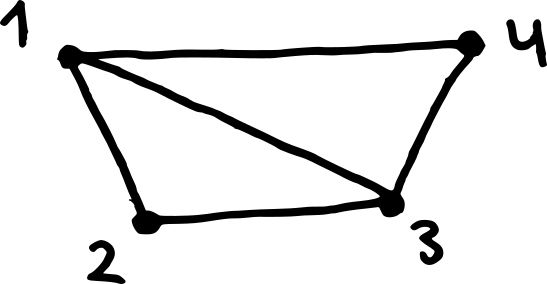
\includegraphics[width=0.25\textwidth]{26}
  \vspace{-4mm}
  \caption{Помеченный граф $G$}
\end{wrapfigure}

\textbf{Пример:} опять рассмотрим тот же граф $G$, $(4,5)$-граф порядка 4 (\textit{Рис. 25}).
\begin{itemize}
 \item $N(1) = \{ 2,3,4 \}$ -- окружение вершины 1;
 \item $N(2) = \{ 1,3 \}$ -- окружение вершины 2;
 \item смежные вершины -- концы рёбер -- 1 и 2, 1 и 3, 1 и 4, 2 и 3, 3 и 4;
 
 \item смежные рёбра -- рёбра $(1,2)$, $(1,3)$, $(1,4)$, рёбра $(2,3)$, $(3,4)$, $(1,3)$, рёбра $(3,4)$, $(1,4)$, рёбра $(1,2)$, $(2,3)$;
 \item инцидентны рёбра $(1,2)$, $(1,3)$, $(1,4)$ с вершиной 1, рёбра $(2,3)$, $(3,4)$, $(1,3)$ с вершиной 3, рёбра $(3,4)$, $(1,4)$ с вершиной 4, рёбра $(1,2)$, $(2,3)$ с вершиной 2;
 \item степени вершин: $\deg 1=3$, $\deg 2=2$, $\deg 3=3$, $\deg 4=2$.
\end{itemize}

\subsubsection{Определение ориентированного графа и его элементов}

Понятие \textit{ориентированного графа} (\textit{орграфа}) описывает более сложную структуру с несимметричными связями аналогично понятию \textit{неориентированного графа}, или просто графа. В технической литературе можно встретить определение ориентированного графа, восходящее опять же к его наглядной интерпретации, а именно: \textit{орграфом называется совокупность вершин и связывающих их дуг, которые обозначаются стрелочками.}

Строгие же теоретико-множественные определения опираются на понятие \textit{упорядоченной пары}. Понятие упорядоченной пары указывает, что важен не только выбор двух элементов, но и их порядок.

Множество упорядоченных пар элементов, взятых из двух множеств $M_1$ и $M_2$ называется \textbf{декартовым произведением} этих множеств, то есть:
\[M_1 \times M_2 = \{ (m_1, m_2): \quad \forall m_1 \in M_1 \land \forall m_2 \in M_2 \} \]

Пусть $V$ -- непустое множество а $V^2 = V \times V$ -- множество упорядоченных пар элементов множества $V$, тогда:
\begin{enumerate}
 \item упорядоченная пара $(V, A)$, где $A$ -- произвольное подмножество множества $V^2$, называется \textbf{ориентированным графом} или \textbf{орграфом};
 \item элементы множества $V$ называются \textbf{вершинами орграфа};
 \item элементы множества $A$ называются \textbf{дугами орграфа};
 \item \textbf{порядком орграфа} называется число его вершин.
\end{enumerate}
\textbf{Обозначения:} Пусть имеется орграф $G$, тогда:
\begin{itemize}
 \item $V(G) = \{ 1, 2, \cdots, n \}$ -- множество вершин;
 \item $|V(G)| = n$ -- количество вершин, порядок орграфа;
 \item $A(G)$ -- множество дуг орграфа;
 \item $|E(G)| = m$ -- число дуг орграфа;
 \item $\irv{u, v}$ -- дуга, где $u$ и $v$ -- концевые вершины, причём первая -- \textit{начало дуги}, а вторая -- \textit{конец}.
\end{itemize}

\textbf{Замечание:} Иногда в литературе вместо термина \textit{дуги} также употребляют термин \textit{рёбра}.

Если у орграфа $|V(G)| = n$, а $|А(G)| = m$, то этот орграф называется $(n, m)$-\textbf{орграфом}. Можно сказать, что, если дуга -- это упорядоченная пара вершин, то орграф $G = V(G) \cup А(G)$ -- это \textit{совокупность вершин и дуг}.

Дуга (ребро) $\irv{v, v}$ или $(v, v)$ с совпадающим началом и концом называется \textbf{петлёй}, а графы \textit{с петлями} называются \textbf{псевдографами}.

\begin{figure}[h]
 \centering
 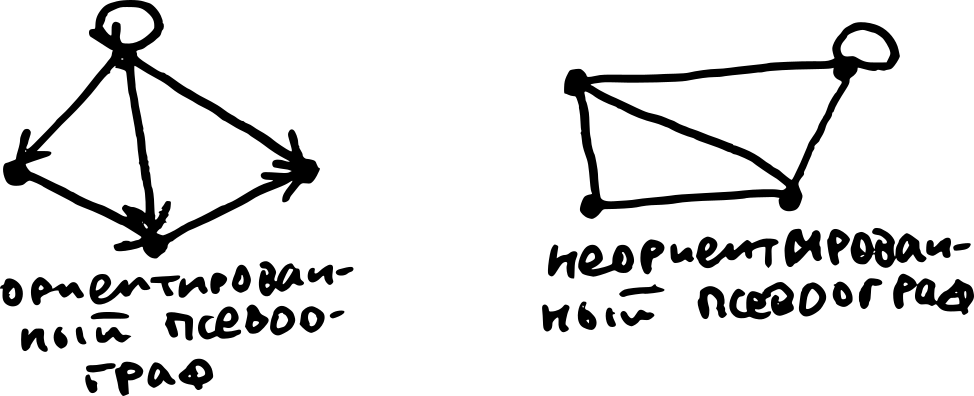
\includegraphics[width=0.35\textwidth]{27}
 \vspace{-4mm}
  \caption{Псевдографы}
\end{figure}

\textbf{Пример:} граф на \textit{Рис. 27} является $(4,6)$-орграфом, его порядок $|V(G)| = 4$, число дуг $|A(G)| = 6$, множество вершин $V(G) = \{ 1,2,3,4 \}$, множество дуг
\[A(G) = \{ \irv{1,2}, \irv{2,3}, \irv{3,4}, \irv{3,1}, \irv{3,4}, \irv{1,4}, \irv{3,3} \}, \]
среди которых одна петля -- дуга $\irv{3,3}$.

\subsubsection{Отношения смежности и инцидентности для орграфов}

Между вершинами существует \textit{отношение смежности}, и между дугами орграфа существует \textit{отношение смежности}, а между вершинами и дугами -- \textit{отношение инцидентности}.

\textbf{Вершина} $u$ орграфа $G$ \textbf{смежная с вершиной} $v$, если дуга $\irv{v, u}$ принадлежит множеству $А$, то есть существует дуга $\irv{v, u}$ орграфа $G$, в противном случае они \textbf{несмежные}. Отношения смежности между вершинами в случае орграфа \textit{несимметричные}.

\textbf{Окружением вершины} $v$ орграфа $G$ называется множество вершин $N(v)$, смежных с вершиной $v$.

\textbf{Степенью вершины} $v$ орграфа $G$ называется $\deg v = |N(v)|$ -- мощность множества $N(v)$. Иными словами, окружение вершины -- это множество смежных вершин, которые являются концами дуг, выходящей из данной вершины, а порядок вершины -- их количество.

\textbf{Дуга} $\irv{v, t}$ орграфа $G$ называется \textbf{смежной с дугой} $\irv{u, v}$, если $\irv{u, v}, \irv{v, t}$ принадлежат множеству $А(G)$ -- множеству дуг орграфа $G$. Отношения смежности для дуг также \textit{несимметричны} для орграфов: смежной первой дуге будет дуга, \textit{начало которой совпадает с концом первой}.

Вершина $v$ и дуга $\irv{u, v}$ \textbf{инцидентны}, когда вершина $v$ -- конец дуги, в противном случае они
\textbf{не инцидентны}. Можно сказать, что всякая вершина \textit{инцидентна} входящим в неё дугам.

\begin{wrapfigure}{r}{0.25\textwidth}
  \centering
  \vspace{2cm}
  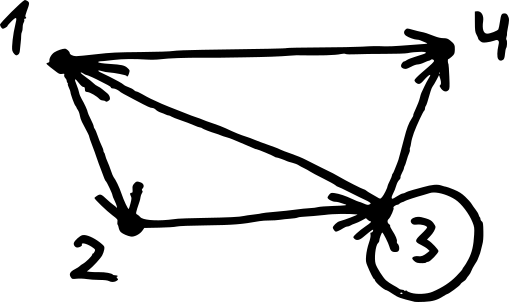
\includegraphics[width=0.25\textwidth]{28}
  \vspace{-4mm}
  \caption{Помеченный орграф $G$}
\end{wrapfigure}

\textbf{Пример:} у помеченного $(4,5)$-орграфа $G$ на \textit{Рис. 27}:
\begin{itemize}
 \item вершина 1 смежная с вершиной 3, 4 -- с вершинами 1 и 3, 2 -- с 1, 3 -- с 2;
 \item дуга $\irv{2,3}$ смежная с дугой $\irv{1,2}$, дуга $\irv{3,4}$ -- с дугой $\irv{2,3}$ и петлёй $\irv{3,3}$, $\irv{1,4}$ -- с $\irv{3,1}$, а петля $\irv{3,3}$ смежная с дугой $\irv{2,3}$;
 \item вершина 1 инцидентна дуге $\irv{3,1}$, вершина 2 инцидентна дуге $\irv{1,2}$, вершина 3 инцидентна дуге $\irv{2,3}$ и петле $\irv{3,3}$, вершина 4 инцидентна дугам $\irv{1,4}$ и $\irv{3,4}$;
 \item окружения вершин: $N(1) = \{ 2,4 \}$, $N(2) = \{ 3 \}$, $N(3) = \{ 1,3 \}$, $N(4) = \varnothing$;
 \item степени вершин $\deg 1=2$, $\deg2=1$, $\deg3=2$, $\deg4=0$.
\end{itemize}

\subsubsection{Мультиграфы}

\begin{figure}[h]
 \centering
 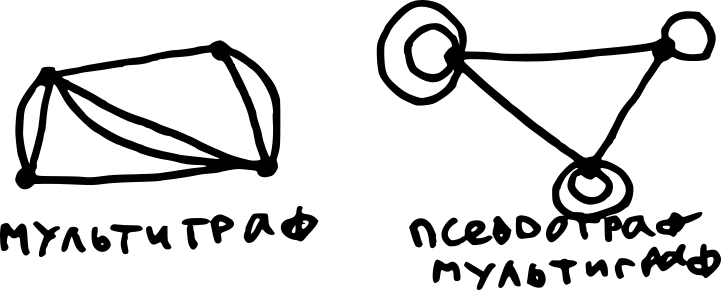
\includegraphics[width=0.35\textwidth]{29}
 \vspace{-3mm}
  \caption{Мультиграфы}
\end{figure}

Граф, у которого паре вершин (или одной вершине) соответствует несколько рёбер или дуг, называется \textbf{мультиграфом}. Если у псевдографа есть две и более петель у одной вершины, он также является \textit{мультиграфом}.

\subsubsection{Полный граф и дополнительный граф}

\begin{wrapfigure}[11]{l}{0.22\textwidth}
  \centering
  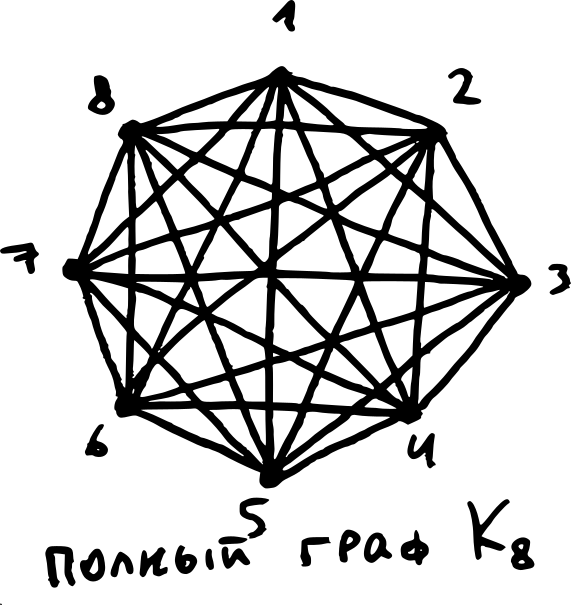
\includegraphics[width=0.22\textwidth]{30}
  \vspace{-7mm}
  \caption{Полный граф $K_8$}
\end{wrapfigure}

\textbf{Полным графом} порядка $n$ называется граф $K_n$, у которого каждая пара вершин соединена ребром.

\textbf{Теорема:} $|E(K_n)| = \frac{n(n-1)}{2}$.

\textbf{Док-во:} Всего в графе $n$ вершин. Из каждой из них выходит $(n-1)$ ребро. Таким образом, получим $n(n-1)$ ребро. Так как каждое ребро относится к двум вершинам, при таком подсчёте оно будет учитываться дважды, поэтому следует поделить на 2. Получим: $\frac{n(n-1)}{2}$.

\textbf{Дополнением графа} $G(V,E)$ или \textbf{дополнительным графом к графу} $G$ называется граф $\bar{G}(V,\bar{E})$, дополняющий исходный граф $G$ до \textit{полного} $K_n$, где $\bar{E} \cup E = V \times V$.

\begin{figure}[h]
 \centering
 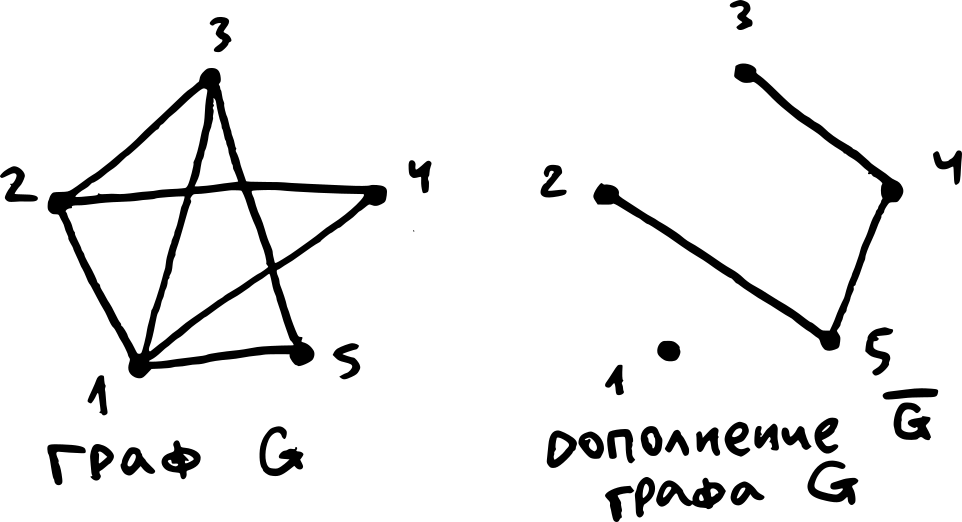
\includegraphics[width=0.4\textwidth]{31}
 \vspace{-4mm}
  \caption{Дополнение графа}
\end{figure}

%\subsection{Основные понятия (продолжение)}

\subsubsection{Однородные графы и их свойства}

Примерами однородных графов могут послужить структуры некоторых молекул, например, бензола, если под вершинами понимать атомы, а под рёбрами -- химические связи, а также структуры некоторых кристаллов, например, алмаза или кремния.

Граф называется \textbf{однородным}, если степени всех его вершин равны. Число, которому равны все степени графа, называется \textbf{степенью однородного графа}. Обозначается как $R_n^k$, где $k$ -- степень каждой вершины, а $n$ -- порядок графа.

\begin{figure}[h]
 \centering
 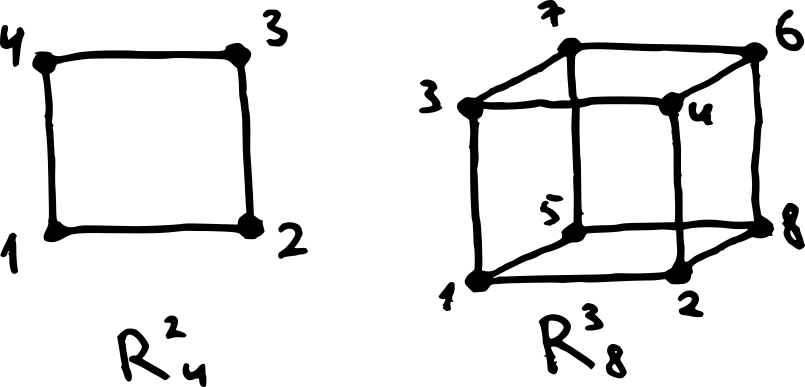
\includegraphics[width=0.4\textwidth]{32}
 \vspace{-3mm}
  \caption{Однородные графы}
\end{figure}

\textbf{Теорема:} В любом однородном графе либо его порядок, либо степень его вершин есть чётное число.

\textbf{Доказательство:} Число рёбер однородного графа $R_n^k$, в котором каждая из $n$ вершин инцидентна $k$ рёбрам, равно $m = \frac{n \cdot k}{2}$, так как каждое ребро инцидентно двум вершинам. Отсюда, так как $m$ -- целое число, вытекает утверждение теоремы.

\subsubsection{Свойства степеней вершин}

В начале заметим, что ниже речь идет о простых неориентированных графах без петель и изолированных вершин.

\textbf{Теорема:} Для любого $(n,m)$-графа $G$ выполняются следующие соотношения:
\begin{enumerate}
 \item сумма всех степеней вершин графа есть чётное число, равное удвоенному количеству рёбер:
 \[2m = \sum_{k=1}^n \deg{(k)}; \]
 \item число вершин нечётной степени в любом графе чётно;
 \item в любом простом графе обязательно найдутся хотя бы две вершины, имеющие одинаковую степень.
\end{enumerate}

\textbf{Доказательство:}
\begin{enumerate}
 \item Степень вершины -- это число смежных вершин, то есть число рёбер, выходящих из данной вершины, следовательно, раз каждое ребро инцидентно двум вершинам, то $2m = \sum \limits_{k=1}^n \deg{(k)}$.
 \item Из первого утверждения вытекает, что сумма степеней всех вершин графа чётная, сумма степеней вершин чётной степени тоже чётное число, следовательно, сумма степеней вершин нечётной степени, как разность чётных чисел, также чётная, что возможно только в случае, когда их количество чётно.
 \item Предположим противное, что все вершины $(n,m)$-графа $G$ имеют разные степени. Тогда $n$ вершин могут иметь $n$ различных степеней единственным образом: от $(n-1)$ до $0$. То есть должна быть изолированная вершина, что противоречит условию простоты графа. Следовательно, предположение неверно, и существуют две вершины с одинаковой степенью.
\end{enumerate}

\subsubsection{Изоморфизм графов}

Это одно из важнейших понятий теории графов, которое для графов является эквивалентным понятию равенства.

Два графа $G$ и $H$ называются \textbf{изоморфными}, если существует \textit{биекция} (взаимно однозначное соответствие) между множествами их вершин, сохраняющее отношение смежности. Обозначается как $G \cong H$.

\begin{figure}[h]
 \centering
 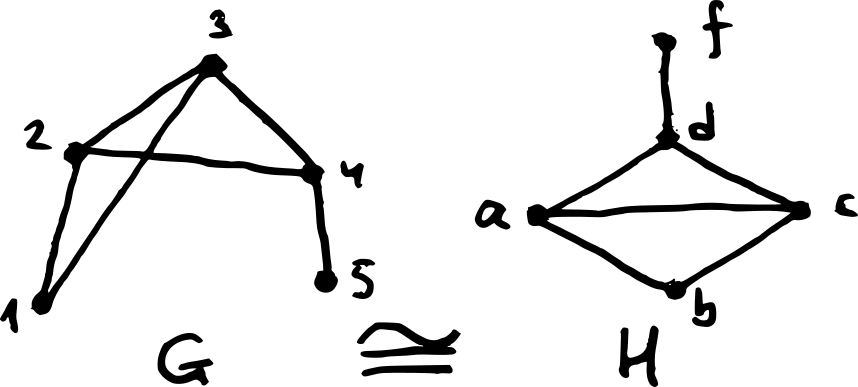
\includegraphics[width=0.4\textwidth]{33}
 \vspace{-4mm}
  \caption{Изоморфные графы}
\end{figure}

Граф называется \textbf{самодополнительным}, если он изоморфен своему дополнению. Два \textbf{самодополнительных} и изоморфных графа представлены на \textit{Рис. 32} и \textit{33}.

\begin{figure}[h]
 \centering
 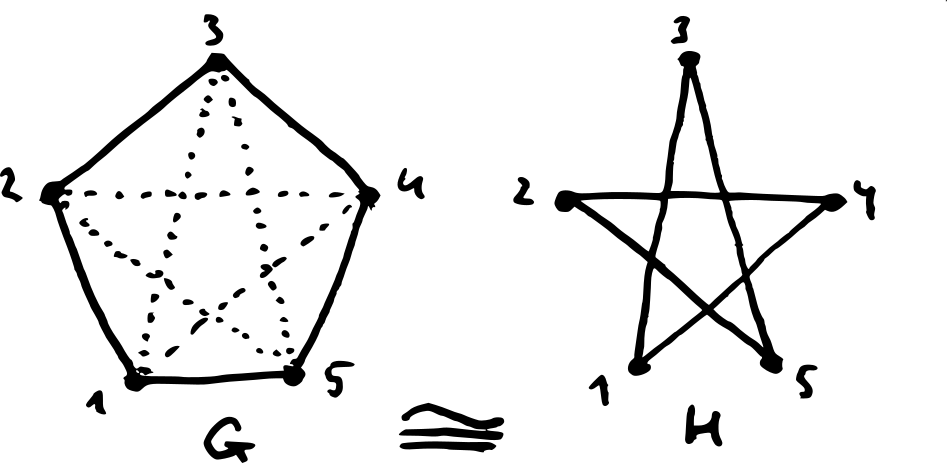
\includegraphics[width=0.4\textwidth]{34}
 \vspace{-4mm}
  \caption{Самодополнительный граф}
\end{figure}

\subsubsection{Подграфы и их виды}

Понятие подграфа как подструктуры важно для анализа графов, но оно отличается от понятия подмножества.

Положим, что даны два графа: $G(V, E)$ и $G_1(V_1, E_1)$.
\begin{enumerate}
 \item Граф $G_1(V_1, E_1)$ называется \textbf{подграфом} графа $G(V, E)$, если $V_1 \subseteq V$, а $E_1 \subseteq E$.
 \item Подграф $G_1(V_1, E_1)$ графа $G(V, E)$ \textbf{остовным}, если $V_1 = V$, а $E_1 \subseteq E$.
 \item Подграф $G_1(V_1, E_1)$ графа $G(V, E)$ \textbf{порождённым}, если для любых вершин $u, v \in V_1$ верно, что $(u, v) \in E_1$ тогда и только тогда, когда $(u, v) \in E$.
 То есть, вершины подграфа есть подмножество вершин основного графа, а рёбра подграфа -- подмножество рёбер основного графа. В \textit{остовной подграф} входят все вершины основного графа. Для \textit{порожденного подграфа} множество рёбер совпадает со множеством рёбер основного графа, инцидентных вершинам подграфа.
\end{enumerate}

\begin{figure}[h]
 \centering
 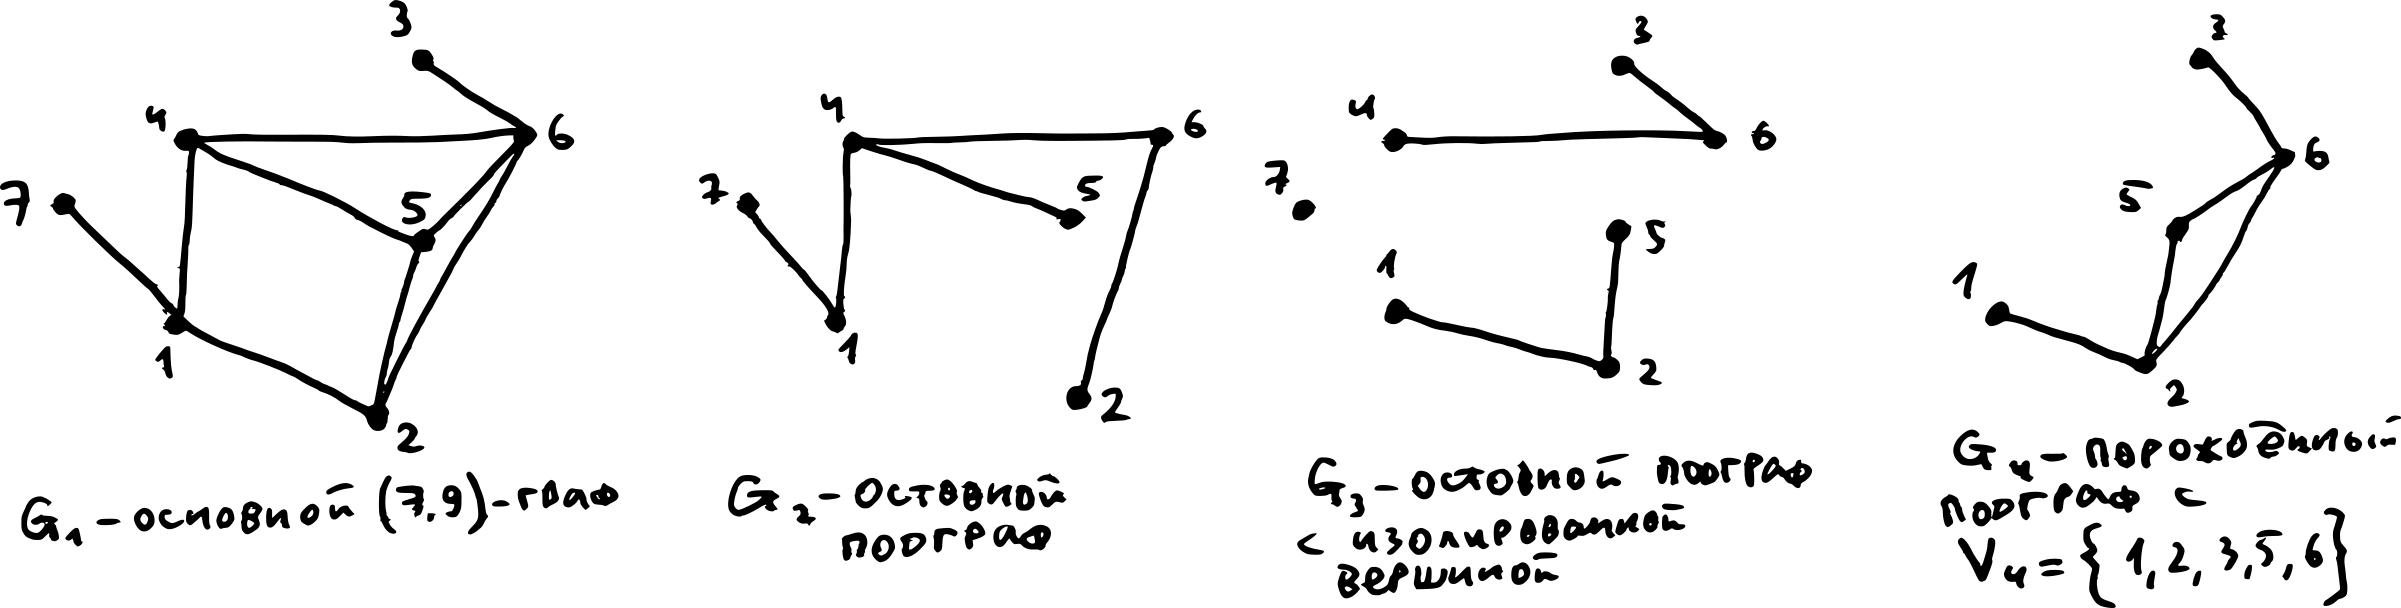
\includegraphics[width=0.9\textwidth]{35}
 \vspace{-4mm}
  \caption{Остовные и порождённые подграфы}
\end{figure}

\subsubsection{Маршруты и частные случаи маршрутов}

Понятие \textit{маршрута} очень важно для определения такой характеристики графов как \textit{связность}, а также для способов их \textit{обхода} и \textit{построения}, \textit{пересчёта элементов} графа. \textit{Связность} -- это характеристика целостности структуры. Для орграфов соответствующие понятия имеют несколько более сложный вид, но здесь будем рассматривать лишь неориентированные графы.
\begin{enumerate}
\item \textbf{Маршрутом} называется последовательность вершин и соединяющих их рёбер графа. Маршрут, соединяющий вершины $v_1$ и $v_n$ обозначается:
\[v_1(v_1,v_2)v_2(v_2,v_3)v_3 \cdots v_{n-1}(v_{n-1},v_n)v_n \]
\item \textbf{Длиной маршрута} называется число входящих в него рёбер. Длина маршрута, соединяющего вершины $v_1$ и $v_n$ обозначается:
\[\rho (v_1(v_1,v_2)v_2(v_2,v_3)v_3 \cdots v_{n-1}(v_{n-1},v_n)v_n) = n \]
\item \textbf{Расстоянием между вершинами} $u$ \textbf{и} $v$ называется длина кратчайшего маршрута между ними. Обозначается как $d(u, v) = \min \rho (u(u, \cdots) \cdots (\cdots, v)v)$.
\end{enumerate}

\begin{wrapfigure}[5]{r}{0.25\textwidth}
  \vspace{-8mm}
  \centering
  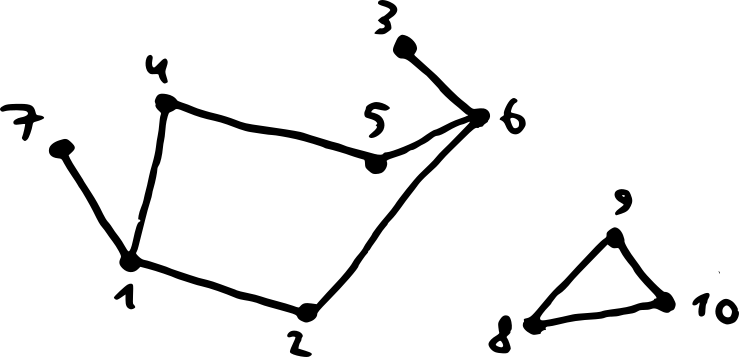
\includegraphics[width=0.25\textwidth]{36}
  \vspace{-7mm}
  \caption{$(10,10)$-граф}
\end{wrapfigure}

\textbf{Пример:} Рассмотрим $(10, 10)$-граф $G$. Из вершины $1$ в вершину $6$ существует 2 маршрута. Первый: $1(1, 2)2(2, 6)6$ длиной $\rho_1=2$ и второй: $1(1, 4)4(4, 5)5(5, 6)6$ длиной $\rho_2=3$, расстояние между вершинами $1$ и $6$ равно $d(1, 6) = 2$. Из $1$ в $10$ нет маршрута, тогда $d(1, 10) = \infty$.

\begin{enumerate}
 \item \textbf{Цепь} -- это маршрут, у которого все рёбра различны (вершины же могут повторяться).
 \item \textbf{Цепь} -- \textbf{простая}, если все вершины, разве что кроме крайних, различны. Обозначается как $P_n$.
 \item \textbf{Маршрут} -- \textbf{циклический}, если конечная вершина совпадает с исходной.
 \item \textbf{Цикл} -- циклическая цепь, или цепь с совпадающими концами.
 \item \textbf{Цикл простой} -- это простая циклическая цепь. Обозначается как $C_n$.
\end{enumerate}

\textbf{Примеры:}

\begin{wrapfigure}{r}{0.2\textwidth}
 \centering
 \vspace{-10mm}
 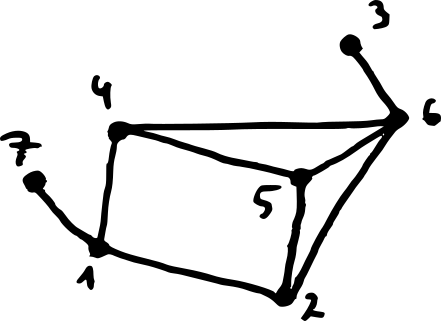
\includegraphics[width=0.2\textwidth]{37}
 \vspace{-4mm}
 \caption{$(7,9)$-граф $G$}
\end{wrapfigure}

Рассмотрим $(7,9)$-граф $G$ на \textit{Рис. 36}. Маршрут
\[7(7,1)1(1,4)4(4,5)5(5,6)6(6,4)4 \]
-- \textit{цепь непростая}, так как вершина 4 встречается дважды. Маршрут
\[7(7,1)1(1,2)2(2,5)5(5,6)6(6,4)4 \]
-- \textit{цепь простая}.

\begin{wrapfigure}{r}{0.25\textwidth}
 \centering
 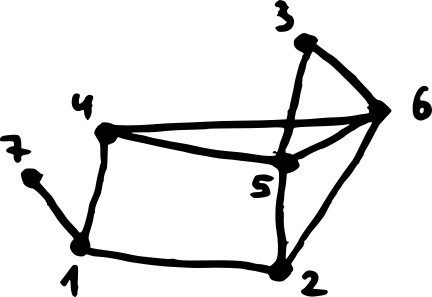
\includegraphics[width=0.25\textwidth]{38}
 \vspace{-4mm}
 \caption{$(7,10)$-граф $G$}
\end{wrapfigure}

Рассмотрим $(7,10)$-граф $G$ на \textit{Рис. 37}. Маршрут
\[7(7,1)1(1,2)2(2,5)5(5,4)4(4,1)1(1,7)7 \]
-- \textit{циклический}, так как совпадают начало и конец маршрута. Маршрут
\[6(6,5)5(5,4)4(4,6)6(6,2)2(2,1)1(1,4)4(4,6)6 \]
-- \textit{цикл}, но \textit{не простой}, так как есть повторяющиеся вершины. Маршрут
\[4(4,1)1(1,2)2(2,5)5(5,4)4 \]
-- \textit{простой цикл}.

\subsubsection{Связные графы и их свойства}

\textbf{Граф связный}, если любые его две несовпадающие вершины соединены маршрутом.

\textbf{Вершины} $u$ и $v$ \textbf{эквивалентны}, если существует связывающий их маршрут или $u=v$. Обозначается как $u \cong v$.

Множество эквивалентных вершин образуют \textbf{класс эквивалентности} или \textbf{компоненту связности}.

Таким образом, всякий граф можно представить в виде объединения классов эквивалентности, не имеющих общих вершин. Используя \textit{простейшие операции над графами} -- а именно стягивание рёбер -- можно получить в итоге пустой граф, состоящий из конечного числа вершин, равных количеству компонент связности. Образно можно представить себе \textit{классы эквивалентности} графа, представив себе нескольких осьминогов, распластавших щупальца-<<рёбра>> на морском дне. И если каждый сожмётся в комок-<<вершину>>, то их будет столько, сколько \textit{компонент связности} у графа.

\textbf{Пример:} У $(10,10)$-графа на \textit{Рис. 38} есть две компоненты связности.

\begin{figure}[h]
 \centering
 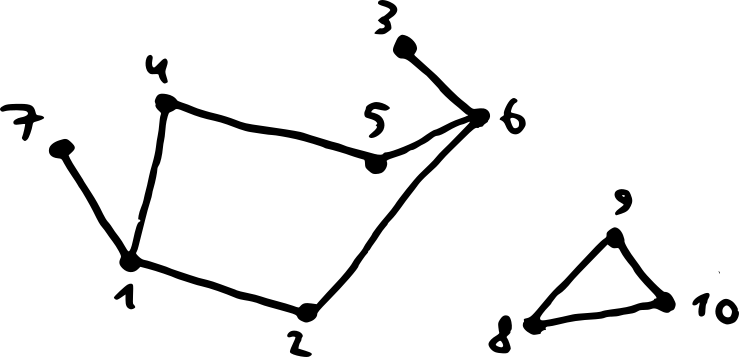
\includegraphics[width=0.35\textwidth]{36}
 \vspace{-4mm}
 \caption{$(10,10)$-граф}
\end{figure}

\textbf{Теорема} (о свойствах связных графов, без док-ва)\textbf{:}
\begin{enumerate}
\item Для любого графа либо он сам, либо его дополнение являются связным графом.
\item Связный граф остаётся связным графом после удаления ребра в том и только том случае, если удалённое ребро принадлежало циклу.
\item При удалении ребра из связного графа, граф либо остается связным, либо распадается на две компоненты связности.
\item В связном графе порядка $n$ число рёбер не меньше, чем $n-1$.
\end{enumerate}

\subsection{Леса, деревья и другие виды графов}

\subsubsection{Деревья и леса}

Особенно часто \textit{деревья} используются в теории планирования и теории алгоритмов.

Граф, в котором \textit{нет циклов} (\textit{ациклической граф}) называется \textbf{лесом}. 

\begin{figure}[h]
 \centering
 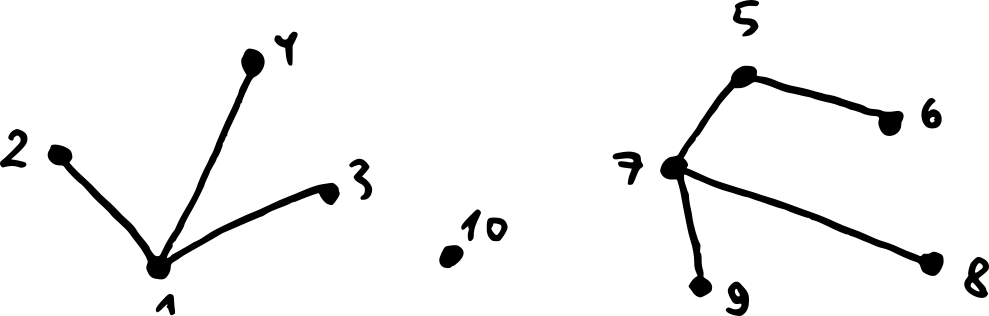
\includegraphics[width=0.35\textwidth]{39}
 \vspace{-4mm}
 \caption{Лес}
\end{figure}

В лесу кроме деревьев могут быть и <<\textit{пеньки}>> -- изолированные вершины.

\begin{wrapfigure}[5]{r}{0.2\textwidth}
  \vspace{-5mm}
  \centering
  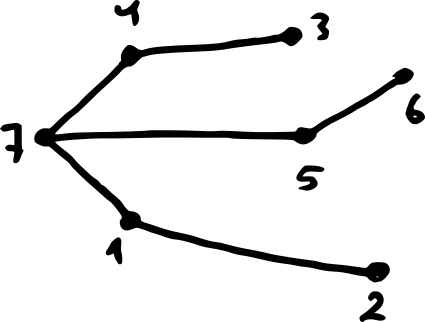
\includegraphics[width=0.2\textwidth]{40}
  \vspace{-9mm}
 \caption{Дерево}
\end{wrapfigure}

\textit{Связный ациклический} граф называется \textbf{деревом}. Обозначается как $T_n$ -- дерево порядка $n$.

Висячие вершины дерева называются \textbf{концевыми вершинами}.

Если остовной подграф некоторого графа является \textit{деревом}, то он называется \textbf{остовным деревом} или \textbf{остовом}.

Необходимые и достаточные условия для того, чтобы граф был деревом, даёт следующая теорема (без доказательства).

\textbf{Теорема} (Об определении дерева)\textbf{:}
Для $(n,m)$-графа $G$ следующие утверждения эквивалентны:
\begin{enumerate}
\item граф $G$ -- дерево;
\item граф $G$ -- связный граф и $m = n – 1$;
\item граф $G$ -- ациклический граф и $m = n – 1$;
\item любые две несовпадающие вершины графа соединены единственной простой цепью.
\end{enumerate}

\textbf{Теорема} (О свойствах дерева)\textbf{:}
В любом дереве порядка $n \geq 2$ имеется не менее двух висячих вершин.

\textbf{Док-во:} Простейшее дерево -- это простая ациклическая цепь. У неё две висячие вершины. При добавлении дополнительных рёбер, которые не образуют циклов, могут появиться только дополнительные висячие вершины.

Задача построения \textit{остова} (\textit{остовного дерева}) актуальна при прокладке сетей связи и дорог, связывающих заданные пункты.

\subsubsection{Корневые деревья}

Есть несколько определений \textit{корневого дерева} для разных типов графов и разных ситуаций.

\textit{Неориентированный} граф называется \textbf{корневым деревом}, если у него выбрана \textbf{корневая вершина}.

Для \textit{неориентированного} дерева в качестве корневой может быть выбрана любая из его вершин, как на \textit{Рис. 41} (слева).

Для \textit{ориентированного} графа существуют два случая выбора корневой вершины: либо эта вершина \textit{нулевой степени}, то есть у неё нет инцидентных дуг (рёбер), тогда эта вершина называется \textbf{истоком} (вершина 1 дерева на \textit{Рис. 41} справа), либо, если в неё только входят все дуги (рёбра), тогда эта вершина называется \textbf{стоком} (вершина 5 дерева на \textit{Рис. 41} справа).

\begin{figure}[h]
 \centering
 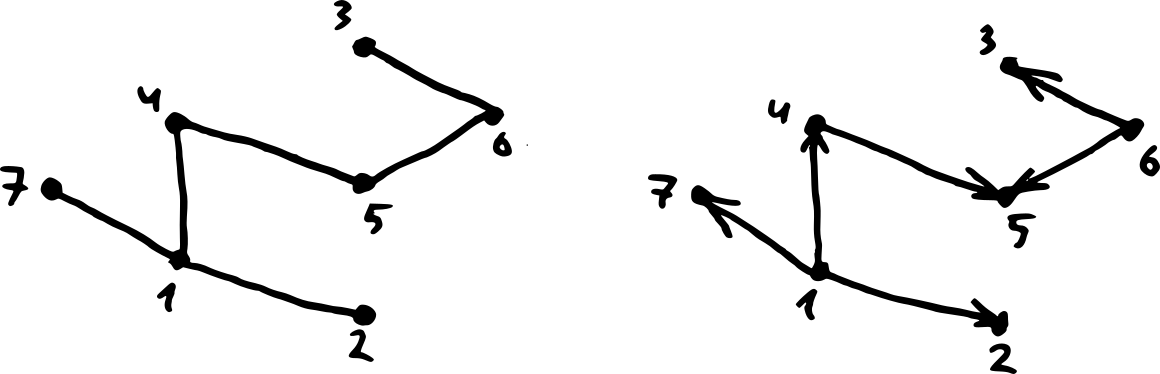
\includegraphics[width=0.45\textwidth]{41}
 \vspace{-4mm}
 \caption{Деревья: неориентированное и ориентированное}
\end{figure}

\subsubsection{Двудольные графы}

Граф $G$ называется \textbf{двудольным графом}, если существует такое разбиение его вершин на две части (\textbf{доли}) такое, что концы каждого ребра принадлежат разным долям.

\begin{figure}[h]
 \centering
 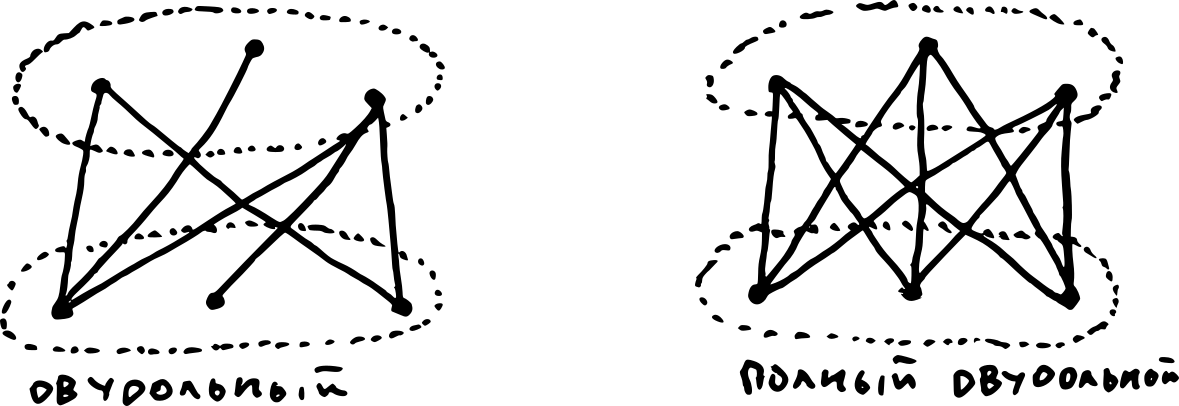
\includegraphics[width=0.45\textwidth]{42}
 \vspace{-4mm}
 \caption{Двудольные графы}
\end{figure}

Например, структура супружеских связей описывается двудольным графом, вершинам которого соответствуют люди, которых можно подразделить на две части: мужей и жён.

Граф называется \textbf{полным двудольным графом}, если у двудольного графа любые две вершины из разных долей смежные. Полный двудольный граф, доли которого состоят из $p$ и $q$ вершин, обозначается $K_{p,q}$.

Следующая теорема (без доказательства) даёт необходимые и достаточные условия.

\textbf{Теорема} (Критерий двудольности)\textbf{:} Граф является двудольным тогда и только тогда, когда он не содержит простых циклов нечётной длины.

\textbf{Док-во:} \textit{Если граф двудольный}, то, чтобы вернуться по замкнутому маршруту -- простому циклу -- в исходную точку по рёбрам, инцидентным всегда паре вершин из разных долей, нужно обязательно пройти по два раза туда и обратно несколько раз, не проходя два раза по одному и тому же ребру, так как цикл простой, следовательно нечётных простых циклов нет.

\textit{Если в графе только простые чётные циклы}, то тогда все вершины, через которые проходят циклы, можно поделить на доли по принципу: нечётные вершины циклов принадлежат одной доле, а чётные другой, начиная с первого цикла. Тогда второй цикл, если он содержит вершины первого, уже имеет тот же порядок нумерации, а если нет общих вершин с первым циклом -- можно назначить произвольно. И далее по индукции. Изолированные вершины или висячие вершины, связанные одиночным ребром, можно приписать к разным долям произвольно. Таким образом получим двудольный граф.

\subsubsection{<<Свадебный переполох>> и теорема Холла}

Наглядное представление о проблеме разбиении графа на доли даёт задача о свадьбах. Рассмотрим некоторое множество юношей, каждый из которых знаком с несколькими девушками. Требуется женить юношей так, чтобы каждый из них сочетался браком со знакомой ему девушкой.

При каком условии эта задача разрешима? Конечно, девушек, знакомых юношам, должно быть не меньше, чем юношей, но одного этого условия недостаточно. Действительно, если один из юношей знаком со всеми девушками, а все остальные юноши знакомы только с одной и той же девушкой, то, если юношей более двух, поженить их невозможно, соблюдая условие знакомства. Если задача о свадьбах разрешима, то любые $k$ из данных юношей должны быть знакомы не менее, чем с $k$ девушками. Удивительным образом это необходимое условие разрешимости задачи оказывается также и достаточным.

\textbf{Теорема о свадьбах} (Холла)\textbf{:} Решение задачи о свадьбах существует тогда и только тогда, когда любые $k$ юношей из данного семейства знакомы в совокупности не менее чем с $k$ девушками.

\textbf{Док-во} (по индукции)\textbf{:} Пусть всего $m$ юношей Предположим, что любые $k$ юношей, $1, \cdots, k < m$, знакомы в совокупности не менее чем с $k+1$ девушкой. Тогда, женив любого юношу на знакомой ему девушке, получим, что любые $k$ из оставшихся $m-1$ юношей будут знакомы по крайней мере с $k$ девушками. Теперь предположим, что имеются $k$ юношей, где $k < m$, знакомых всего с $k$ девушками. Этих юношей женить можно. Остаются еще $m - k$ из них. Исключим из рассмотрения тех девушек, на которых женились эти юноши, и проверим, что любые $\ell$ юношей из оставшихся знакомы не менее чем с $\ell$ оставшимися девушками. Предположим противное. Пусть $B'$ -- это множество из $k$ юношей, знакомых в совокупности ровно с $k$ девушками. Рассмотрим множество $B^{\prime \prime}$ каких-то $\ell$ юношей, которые знакомы менее, чем с $\ell$ из оставшихся девушек, пусть $B = B' \cup B^{\prime \prime}$. Множество $B$ состоит из $k + \ell$ юношей, которые знакомы в совокупности менее, чем с $k + \ell$ девушками, что противоречит условию теоремы. Таким образом, условие теоремы Холла выполнено и для множества из $m - k$ оставшихся юношей (и оставшихся девушек), поэтому, в силу индукционного предположения, оставшихся юношей также можно поженить.

Теорема Холла \textit{на языке теории графов}. Напомним, что граф называется двудольным, если множество его вершин можно разбить на такие два подмножества $V_1$ и $V_2$, что любое ребро рассматриваемого графа соединяет вершину из $V_1$ с вершиной из $V_2$.

\textbf{Паросочетание} из $V_1$ в $V_2$:
\begin{enumerate}
\item набор $M$ рёбер двудольного графа, такой что никакие два ребра из этого набора не имеют общих вершин и для всякой вершины $v \in V_1$ найдется инцидентное к ней ребро $\ell \in M$;
\item инъективное (однозначное) отображение $\varphi: V_1 \to V_2$, что для любой вершины $v \in V_1$ существует ребро, соединяющее вершины $v$ и $\varphi (v)$.
\end{enumerate}

\begin{figure}[h]
 \centering
 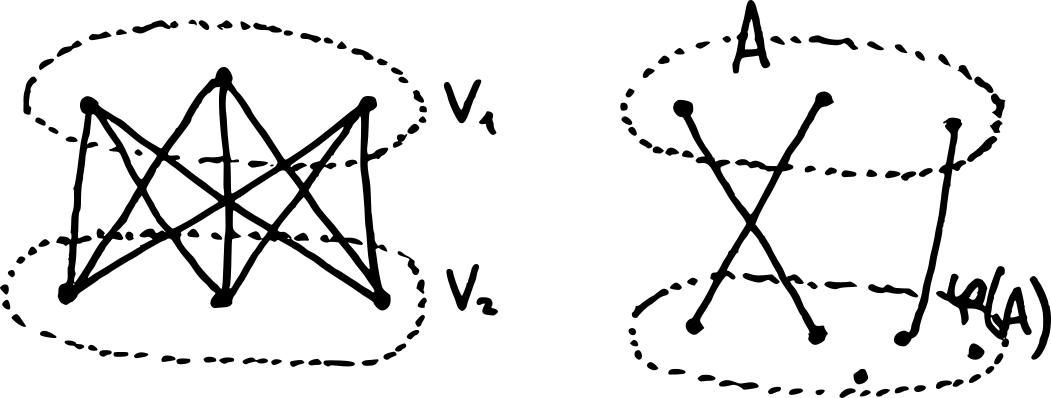
\includegraphics[width=0.45\textwidth]{43}
 \vspace{-4mm}
 \caption{Двудольные граф (слева) и паросочетание $V_1 \to V_2$ (справа)}
\end{figure}

В задаче о свадьбах двудольный граф возникает совершенно естественно. Пусть $V_1$ -- это множество юношей, $V_2$ -- множество девушек. Если юноша $m \in V_1$ и девушка $f \in V_2$ знакомы друг с другом, то пара $\{ m,f \}$ является ребром графа. Паросочетание $M$ из $V_1$ в $V_2$ в таком графе это и есть множество $\{ u,f \}$ супружеских пар, в которых участвуют все юноши. Введём ещё одно обозначение. Для всякого подмножества $A \subset V_1$ через $\Phi (A)$ будем обозначать множество всех вершин $w \in V_2$, для которых существует вершина $u \in  A$, соединённая ребром с вершиной $w$. Ясно, что если $\varphi$ -- паросочетание из $V_1$ в $V_2$, то $\varphi (A) \subset \Phi (A)$. В задаче о свадьбах $\Phi (A)$ -- это множество девушек, с которыми знакомы в совокупности юноши из множества $A$. Тогда теорема Холла на языке графов равносильна следующему утверждению.

\textbf{Теорема:} Пусть $G = (V,E)$ -- это двудольный граф, тогда паросочетание из $V_1$ в $V_2$ существует тогда и только тогда, когда для любого подмножества $A \subset V_1$ справедливо неравенство $|\Phi (A)| > |A|$.

\subsection{Матрицы, ассоциированные с графами}

Ассоциированными матрицами называют матрицы \textit{смежности} и \textit{инцидентности}. Они позволяют задать граф с помощью матриц. Таким образом, можно перейти от картинки, схемы к <<числу>>.

\subsubsection{Матрица смежности и инцидентности для неориентированного графа}

Матрица смежности позволяет однозначно задать граф с точностью до круговой перестановки меток вершин. Но если граф \textit{помеченый}, то он задаётся однозначно матрицей смежности.

\textbf{Матрицей смежности помеченного графа} $G$ порядка $n$ называется квадратная симметричная матрица $А_n$, определяемая как:
\[A_n = \left[ a_{ij} \right]_{i,j=1}^n, \quad \textrm{где } a_{ij} = \begin{cases} 1, & \textrm{если вершины } i,j \textrm{ смежные}; \\ 0, & \textrm{если вершины } i,j \textrm{ несмежные}. \end{cases} \]
Матрица смежности помеченного графа -- \textit{симметричная}, то есть совпадающая со своей транспонированной.

\textbf{Матрицей смежности помеченного мультиграфа} $G$ порядка $n$ называется квадратная матрица $n$-го порядка:
\[A_n = \left[ a_{ij} \right]_{i,j=1}^n, \quad \textrm{где } a_{ij} = \begin{cases} k, & \textrm{если вершины } i,j \textrm{ связывают } k \textrm{ рёбер}; \\ 0, & \textrm{если вершины } i,j \textrm{ несмежные}. \end{cases} \]

Это определение -- обобщение первого, матрица смежности мультиграфа тоже \textit{симметричная}.

\textbf{Замечание:} У матрицы смежности псевдографа на главной диагонали вместо нулей стоит удвоенное количество петель при $i$-й вершине, $i=\bar{1,n}$.

\textbf{Примеры:}

\begin{figure}[h]
 \centering
 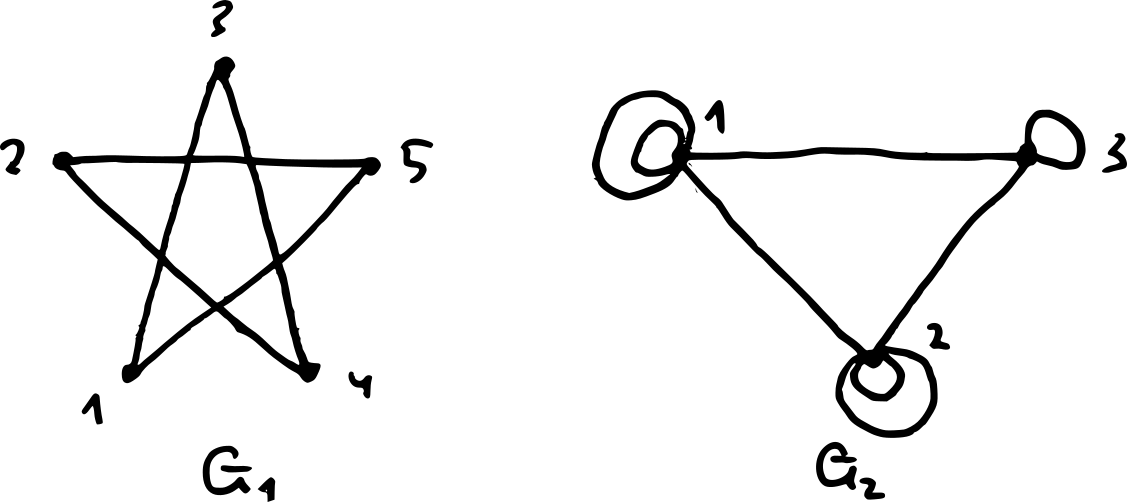
\includegraphics[width=0.5\textwidth]{44}
 \vspace{-3mm}
 \caption{Графы $G_1$ и $G_2$}
\end{figure}

\[A_5(G_1) = \begin{pmatrix}
0 & 0 & 1 & 0 & 1 \\ 0 & 0 & 0 & 1 & 1 \\ 1 & 0 & 0 & 1 & 0 \\ 0 & 1 & 1 & 0 & 0 \\ 1 & 1 & 0 & 0 & 0 
\end{pmatrix} \hspace{2cm}
A_3(G_2) = \begin{pmatrix}
4 & 1 & 1 \\ 1 & 4 & 1 \\ 1 & 1 & 2
\end{pmatrix} \]

Если помеченными в графе оказываются не только вершины, но и дуги (рёбра), то можно задать матрицу \textit{инцидентности}.

\textbf{Матрицей инцидентности} $(n,m)$-графа $G$ называется прямоугольная матрица размером $n \times m$:
\[I = \left( i_{kl} \right)_{k,l=1}^{n,m}, \quad \textrm{где } i_{kl} = \begin{cases} 1, & \textrm{если вершина } k \textrm{ и дуга } l \textrm{ инцидентны}; \\ 0, & \textrm{если вершина } k \textrm{ и дуга } l \textrm{ не инцидентны}. \end{cases} \]

\textbf{Пример:} Матрица инцидентности $(6,8)$-графа $G$ (строки соответствуют вершинам, столбцы -- рёбрам):

\begin{wrapfigure}[0]{r}{0.25\textwidth}
  \centering
  \vspace{-10mm}
  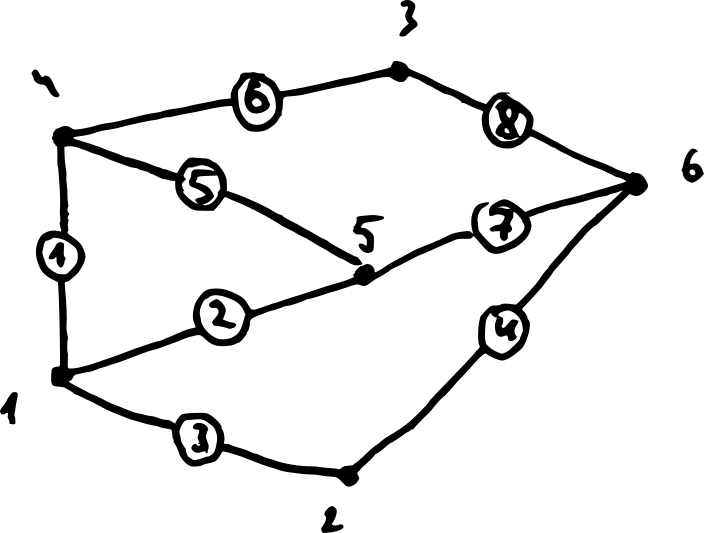
\includegraphics[width=0.25\textwidth]{45}
  \vspace{-8mm}
 \caption{$(6,8)$-граф $G$}
\end{wrapfigure}

\[I = \begin{pmatrix}
1 & 1 & 1 & 0 & 0 & 0 & 0 & 0 \\
0 & 0 & 1 & 1 & 0 & 0 & 0 & 0 \\
0 & 0 & 0 & 0 & 0 & 1 & 0 & 1 \\
1 & 0 & 0 & 0 & 1 & 1 & 0 & 0 \\
0 & 1 & 0 & 0 & 1 & 0 & 1 & 0 \\
0 & 0 & 0 & 1 & 0 & 0 & 1 & 1 \\
\end{pmatrix} \]

\textbf{Замечание:} Матрица смежности задаёт граф с точностью до изоморфизма.

Графы $G$ и $H$ изоморфны тогда и только тогда, когда их матрицы смежности (инцидентности) получаются одна из другой произвольными перестановками строк и столбцов.

Для \textit{ориентированных} графов матрицы смежности и инцидентности \textit{определяются иначе}. Заметим, что в литературе встречаются разные способы задания матриц под одним и тем же названием.

\subsubsection{Матрица смежности и инцидентности для ориентированного графа}

Определения матриц смежности и инцидентности для орграфов очень похожи с определениями для графов, но различаются из-за особенностей определения отношений смежности и инцидентности для орграфов.

\textbf{Матрицей смежности орграфа} $G$ $n$-го порядка называется квадратная матрица $n$-го порядка:
\[A_n = \left( a_{ij} \right)_{i,j=1}^{n}, \quad \textrm{где } a_{ij} = \begin{cases} 1, & \textrm{если вершина } j \textrm{ смежная вершине } i; \\ 0, & \textrm{если вершина } j \textrm{ несмежная } i. \end{cases} \]

\textbf{Пример:}

\begin{wrapfigure}[0]{r}{0.25\textwidth}
  \vspace{-12mm}
  \centering
  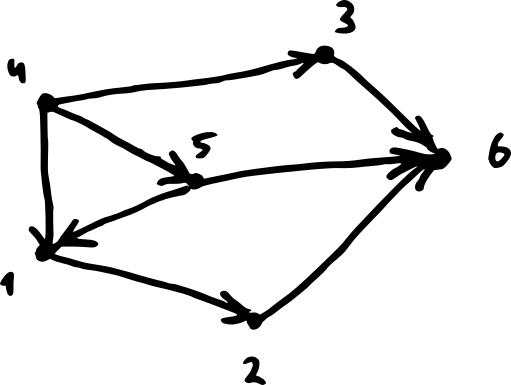
\includegraphics[width=0.25\textwidth]{46}
  \vspace{-7mm}
 \caption{$(6,8)$-орграф}
\end{wrapfigure}

\[A_6 = \begin{pmatrix}
0 & 1 & 0 & 0 & 0 & 0 \\
0 & 0 & 0 & 0 & 0 & 1 \\
0 & 0 & 0 & 0 & 0 & 1 \\
1 & 0 & 1 & 0 & 1 & 0 \\
1 & 0 & 0 & 0 & 0 & 1 \\
0 & 0 & 0 & 0 & 0 & 0 \\
\end{pmatrix} \]

Матрицей смежности мультиорграфа $n$-го порядка $G$ называется квадратная матрица $n$-го порядка:
\[A_n = \left( a_{ij} \right)_{i,j=1}^{n}, \quad \textrm{где } a_{ij} = \begin{cases} k, & \textrm{то есть число дуг, начало которых в вершине } i, \textrm{ а конец в } j; \\ 0, & \textrm{если вершина } j \textrm{ несмежная } i. \end{cases} \]

\newpage

\textbf{Пример:}

\begin{wrapfigure}[0]{r}{0.25\textwidth}
  \vspace{-13mm}
  \centering
  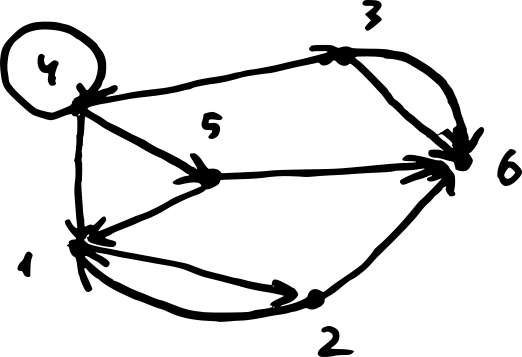
\includegraphics[width=0.25\textwidth]{47}
  \vspace{-8mm}
 \caption{Мульти-псевдоорграф}
\end{wrapfigure}

\[A_6 = \begin{pmatrix}
0 & 1 & 0 & 0 & 0 & 0 \\
1 & 0 & 0 & 0 & 0 & 1 \\
0 & 0 & 0 & 0 & 0 & 2 \\
1 & 0 & 1 & 1 & 1 & 0 \\
1 & 0 & 0 & 0 & 0 & 1 \\
0 & 0 & 0 & 0 & 0 & 0 \\
\end{pmatrix} \]

Если помеченными в орграфе оказываются не только вершины, но и дуги (рёбра), то можно задать \textit{матрицу инцидентности}.

\textbf{Матрицей инцидентности} $(n,m)$-\textbf{орграфа} $G$ называется прямоугольная матрица:
\[I_{n \times m} = \left( i_{kl} \right)_{k,l=1}^{n,m}, \quad \textrm{где } i_{kl} = \begin{cases} +1, & \textrm{если вершина } k \textrm{ -- начало дуги } l; \\ -1, & \textrm{если вершина } k \textrm{ -- конец дуги } l; \\ 0, & \textrm{если вершина } k \textrm{ не является ни началом, ни концом дуги } l. \end{cases} \]

Это определение подходит и для мультиорграфов, так как помечаются все дуги (рёбра).

\textbf{Примеры:}

\begin{wrapfigure}[0]{r}{0.25\textwidth}
  \centering
  \vspace{-8mm}
  \includegraphics[width=0.25\textwidth]{48}
  \vspace{-6mm}
 \caption{$(6,8)$-орграф}
\end{wrapfigure}

\begin{align*}
I(G_3) = \begin{pmatrix}
1 & 0 & 0 & -1 & 0 & 0 & -1 & 0 \\
-1 & 1 & 0 & 0 & 0 & 0 & 0 & 0 \\
0 & 0 & 1 & 0 & -1 & 0 & 0 & 0 \\
0 & 0 & 0 & 1 & 1 & 1 & 0 & 0 \\
0 & 0 & 0 & 0 & 0 & -1 & 1 & 1 \\
0 & -1 & -1 & 0 & 0 & 0 & 0 & -1 \\
\end{pmatrix} &&
\end{align*}

\begin{wrapfigure}[0]{r}{0.22\textwidth}
  \centering
  \vspace{-2mm}
  \includegraphics[width=0.22\textwidth]{49}
  \vspace{-5mm}
 \caption{$(6,10)$-мультиорграф}
\end{wrapfigure}

\begin{align*}
I(G_4) = \begin{pmatrix}
1 & -1 & 0 & 0 & 0 & -1 & 0 & 0 & 0 & -1 \\
-1 & 1 & 1 & 0 & 0 & 0 & 0 & 0 & 0 & 0 \\
0 & 0 & 0 & 1 & 1 & 0 & -1 & 0 & 0 & 0 \\
0 & 0 & 0 & 0 & 0 & 1 & 1 & 1 & 0 & 0 \\
0 & 0 & 0 & 0 & 0 & 0 & 0 & -1 & 1 & 1 \\
0 & 0 & -1 & -1 & -1 & 0 & 0 & 0 & -1 & 0 \\
\end{pmatrix} &&
\end{align*}

\subsubsection{Матрица Кирхгоффа}

Существует ещё один вид матриц, придуманный Робертом Кирхгофом, немецким ученым и инженером 19-го века, основоположником современной электротехники. Матрицы Кирхгофа позволяют в частности найти число остовов для данного графа.

\textbf{Матрицей Кирхгофа помеченного графа} порядка $n$ называется квадратная матрица порядка $n$:
\[K_n = \left( k_{ij} \right)_{i,j=1}^{n}, \quad \textrm{где } k_{ij} = \begin{cases} -1, & \textrm{если вершины } i, j \textrm{ смежны}; \\ 0, & \textrm{если } i \not= j, \textrm{ и вершины } i,j \textrm{ несмежны}; \\ \deg(i), & \textrm{если } i=j. \end{cases} \]

\newpage

\textbf{Пример:}

\begin{wrapfigure}[0]{r}{0.25\textwidth}
  \vspace{-1mm}
  \centering
  \includegraphics[width=0.25\textwidth]{50}
  \vspace{-4mm}
 \caption{$(6,8)$-граф}
\end{wrapfigure}

\[K_6 = \begin{pmatrix}
3 & -1 & 0 & -1 & -1 & 0 \\
-1 & 2 & 0 & 0 & 0 & -1 \\
0 & 0 & 2 & -1 & 0 & -1 \\
-1 & 0 & -1 & 3 & -1 & 0 \\
-1 & 0 & 0 & -1 & 3 & -1 \\
0 & -1 & -1 & 0 & -1 & 3 \\
\end{pmatrix} \]

Подводя итог, можно утверждать, что:
\begin{itemize}
\item графы изоморфны тогда и только тогда, когда их матрицы смежности вершин получаются друг из друга одинаковыми перестановками строк и столбцов;
\item графы изоморфны тогда и только тогда, когда их матрицы инцидентности получаются друг из друга произвольными перестановками строк и столбцов;
\item графы изоморфны тогда и только тогда, когда их матрицы Кирхгофа получаются друг из друга одинаковыми перестановками строк и столбцов.
\end{itemize}

Таким образом, если граф \textit{непомеченный}, то он восстанавливается по ассоциированным матрицам с точностью до перестановки строк и столбцов этих матриц.

\textbf{Замечание:} Между $I$, матрицей инцидентности орграфа, и $K$, матрицей Кирхгофа для соответствующего неориентированного графа, существует простая связь: $K = I \times I^T$.

\subsubsection{Матричная теорема о деревьях}

\textbf{Теорема} (без док-ва)\textbf{:} Граф $G$ связный помеченный граф. $K$ -- его матрица Кирхгофа. Тогда:
\begin{enumerate}
\item все алгебраические дополнения матрицы $K$ равны между собой;
\item их значение равно количеству остовных деревьев графа $G$.
\end{enumerate}

\textbf{Пример:} Рассмотрим ещё раз граф с \textit{Рис. 50}. Подсчитаем два алгебраических дополнения, убедимся в верности теоремы и определим заодно количество \textit{остовных деревьев} или \textit{остовов}:
\[K_{11} = (-1)^1+1 \begin{vmatrix}
2 & 0 & 0 & 0 & -1 \\
0 & 2 & -1 & 0 & -1 \\
0 & -1 & 3 & -1 & 0 \\
0 & 0 & -1 & 3 & -1 \\
-1 & -1 & 0 & -1 & 3 \\
\end{vmatrix} = 35; \hspace{5mm}
K_{44} = (-1)^4+4 \begin{vmatrix}
3 & -1 & 0 & -1 & 0 \\
-1 & 2 & 0 & 0 & -1 \\
0 & 0 & 2 & 0 & -1 \\
-1 & 0 & 0 & 3 & -1 \\
0 & -1 & -1 & -1 & 3 \\
\end{vmatrix} = 35 \]
Таким образом, всего можно построить 35 остовных деревьев.

\subsection{Плоские графы, формула Эйлера и задача Эйлера}

\subsubsection{Плоские графы}

Граф называется \textbf{плоским}, если никакие два его ребра не пересекаются.

Граф называется \textbf{планарным}, если он \textit{изоморфен} некоторому плоскому графу.

\begin{figure}[h]
 \centering
 \includegraphics[width=0.35\textwidth]{51}
 \vspace{-3mm}
 \caption{Плоский и планарный графы}
\end{figure}

\textbf{Теорема:} Любой планарный граф допускает представление, в котором все рёбра являются отрезками.

\textbf{Гранью плоского графа} называется максимальное по включению множество точек плоскости, любые две из которых можно соединить непрерывной кривой, не пересекающей ребра графа. Обозначается строчными латинскими буквами: $a, b, c, \cdots$.

\textbf{Пример:}

\begin{figure}[h]
 \centering
 \includegraphics[width=0.35\textwidth]{52}
 \vspace{-4mm}
 \caption{Грани плоского графа}
\end{figure}

Четыре области: конечные -- $a,b,c$ и бесконечная -- $d$, являются гранями $(7,9)$-графа.

Характеристикой Эйлера графа $G$ называется число, равное $n-m+f$, где $n$ -- порядок графа, $m$ -- число рёбер, $f$ -- число граней:
\[E_G = n - m + f \]

\textbf{Теорема Эйлера} (без док-ва)\textbf{:} Для всякого связного плоского графа характеристика Эйлера равна 2.

\textbf{Примеры:}
\begin{enumerate}
\item Для графа на \textit{Рис. 53} (слева) $n = 7$, $m = 9$, $f = 4 \quad \Rightarrow \quad  E_G = 7-9+4 = 2$.
\item Для любого дерева $T_n$: $m=n-1$, $f=1$, $E_G=n-(n-1)+1=2$.
\end{enumerate}

\subsubsection{Задача Эйлера}

Возвращаемся к задаче о кёнигсбергских мостах в терминах современной теории графов.

\textbf{Эйлеровым циклом} называется цикл, содержащий все рёбра графа.

\textbf{Эйлеровым графом} называется граф, если в нём существует \textit{эйлеров цикл}.

\textbf{Теорема} (без док-ва)\textbf{:} Критерий эйлеровости графа: граф является эйлеровым тогда и только тогда, когда он не содержит вершин нечётной степени.

\newpage

\textbf{Примеры:}

\begin{figure}[h]
 \centering
 \includegraphics[width=0.5\textwidth]{53}
 \vspace{-4mm}
 \caption{Эйлеров граф (слева) и кёнигсбергские мосты (справа)}
\end{figure}

Рассмотрим степени вершин $\deg 1=2, \deg 2=2, \deg 3=2, \deg 4=2, \deg 5=2, \deg 6=4, \deg 7=2, \deg 8=6$ -- в этом графе все вершины чётные, поэтому есть \textit{эйлеров цикл}:
\[8(8,1)1(1,7)7(7,4)4(4,8)8(8,2)2(2,6) \]
\[6(6,5)5(5,8)8(8,6)6(6,3)3(3,8)8 \]

В задаче о кёнигсбергских мостах: $\deg A=5 \deg B=3, \deg C=3, \deg D=3$, следовательно граф не эйлеров, и обойти мосты нельзя, пройдя по каждому только раз.

\section{Методы вычислений: основные понятия и задачи}

\subsection{Введение}

В узком смысле под методами вычислений в математике понимается совокупность типовых вычислительных задач и методов их решения, опирающихся на результаты всех остальных математических дисциплин, в первую очередь математического анализа, функционального анализа, алгебры, теории чисел, теории дифференциальных уравнений и т.д. Это понятно, так как любая математическая задача в конце концов сводится к необходимости получить <<число>>.

В более широком смысле сейчас вычислительные методы понимаются как \textit{метод математического моделирования}, который включает в себя кроме непосредственно вычислительной задачи ещё и \textit{создание математической модели изучаемого объекта}. Для этого, приняв \textit{упрощающие предположения} (например, в астрономии Земля принимается за точку, а в классической механике -- за бесконечную плоскость), составляют уравнения на соответствующем уровне, описывающие эволюцию и основные свойства этой системы. Здесь \textit{наука вычислять} переходит в \textit{искусство строить модели}. Они должны быть максимально простыми, чтобы быть понятными и технически решаемыми, но достаточно сложными, чтобы не потерять определяющих качеств системы, выявить основное. Для этого требуется глубокое изучение соответствующей предметной области.

Предельно обобщая, задача состоит в том, чтобы определить, \textit{что} нужно вычислить (постановка задачи, математическая модель), \textit{как}, по какому алгоритму вычислить (какой метод вычислений, какой алгоритм применить), \textit{при каких условиях} этот алгоритм приведёт к истинному решению (устойчивость алгоритма), \textit{с какой точностью вычислить} (определить абсолютную и/или относительную погрешность полученных
результатов, которая в свою очередь зависит от точности входных данных) и, вообще, \textit{существует ли однозначное решение} задачи и \textit{непрерывная зависимость от параметров задачи} (установить разрешимость и корректность постановки задачи). Кроме того возникает еще и <<экономический>> вопрос: а \textit{какой ценой}, за какое время, с помощью каких ресурсов можем решить эту задачу (скорость сходимости алгоритма)? Для ответов на эти
вопросы и привлекается вся мощь математики. С какой-то точки зрения вся математика работает на методы вычислений.

Крайне актуальная цитата из <<Вычислительных методов для инженеров>> гласит:
\begin{displayquote}
Само по себе использование ЭВМ не только не освобождает от необходимости глубоко осмыслить решаемую проблему, но и заставляет уделять постановке задачи гораздо больше внимания... Вычислительный эксперимент не противоречит натурному эксперименту или классическому математическому анализу задачи, а находится с ними в органическом единстве.
\end{displayquote}

Таким образом подтверждается старая истина философии: <<человек -- мера всех вещей>>. Только грамотные люди со знанием дела могут использовать в полной мере такое сложное орудие труда, каковым является современная вычислительная машина.

На протяжении курса высшей математики уже рассматривались примеры вычислительных задач: задачи интерполяции с помощью многочлена Лагранжа, вычисление значений функции с помощью формулы Тейлора, приближённое представление
функций из различных классов с помощью рядов Тейлора и Фурье. Рассмотрим подробнее некоторые из этих задач.

\subsection{Методы приближённых вычислений значений функции}

\subsubsection{Вычисление значений элементарных функций}

Практически для всех элементарных функций, кроме многочленов, приходится для вычисления их значений применять приближённые методы, прежде всего ряды Тейлора-Маклорена.

\begin{enumerate}
 \item $\mathrm{e}^x = \sum \limits_{k=1}^n \frac{x^k}{k!} + o(x^n) = 1 + x + \frac{x^2}{2!} + \frac{x^3}{3!} + \cdots + \frac{x^n}{n!} + o(x^n), \quad \forall x \in \mathbb{R}$;
 \item $\sin x = \sum \limits_{k=0}^n (-1)^k \frac{x^{2k+1}}{(2k+1)!} + o(x^{2n+1}) = x - \frac{x^3}{3!} + \frac{x^5}{5!} - \cdot \pm \frac{x^{(2n+1)}}{(2n+1)!} + o(x^{2n+1}), \quad \forall x \in \mathbb{R}$;
 \item $\cos x = \sum \limits_{k=0}^n (-1)^k \frac{x^{2k}}{(2k)!} + o(x^{2n}) = 1 - \frac{x^2}{2!} + \frac{x^4}{4!} - \cdots \pm \frac{x^{(2n)}}{(2n)!} + o(x^{2n}), \quad \forall x \in \mathbb{R}$;
 \item $\ln (1+x) = \sum \limits_{k=1}^n \frac{(-1)^{n-1}x^n}{n} + o(x^n) = x - \frac{x^2}{2} + \frac{x^3}{3} - \cdots \pm \frac{x^n}{n} + o(x^n), \quad \forall x \in (-1, 1]$;
 \item $(1+x)^{\alpha} = 1+\alpha x + \frac{\alpha (\alpha - 1)x^2}{2!} + \frac{\alpha (\alpha - 1)(\alpha - 2)x^3}{3!} + \cdots + \frac{\alpha (\alpha - 1) \cdots (\alpha - (n-1))x^n}{n!} + o(x^n), \quad \forall x \in (-1, 1)$.
\end{enumerate}

Погрешность вычислений определяется из теоремы о ряде Тейлора вида
\[f(x) = \sum_{k=0}^n \frac{f^{(k)}(x_0)}{k!} (x-x_0)^k + R_n(x) \]
как модуль остатка ряда и выражается как:
\[R_n(x) = \frac{(x-x_0)^{n+1}}{(n+1)!} f^{(n+1)} [x_0 + \theta (x-x_0)], \quad \theta \in (0, 1). \]

\textbf{Замечание:} Для вычисления значений функций при $x \gg 0$ нужно использовать свойства функций, чтобы привести аргумент к значениям, близким к нулю, чтобы ускорить сходимость алгоритма, то есть уменьшить $n$, количество требуемых слагаемых, чтобы достичь требуемой точности.

\textbf{Примеры:}
\begin{enumerate}
 \item $\sin 3 = \sin (\pi - x) = \sin x, \quad x = \pi - 3 \approx 0.1415\cdots$;
 \item $\eu^{4.5} = \eu^{4+0.5} = \eu^4 \cdot \eu^{0.5}, \quad x=0.5$;
 \item $\sqrt{5} = \sqrt{4+1} = 2\sqrt{1+\tfrac{1}{4}} = 2(1+\tfrac{1}{4})^{\tfrac{1}{2}}, \quad x = \tfrac{1}{4}$.
\end{enumerate}

\textbf{Замечание:} Для сложных функций (суперпозиций) приходится применять переразложение функций с помощью рядов Тейлора или вычислять его коэффициенты непосредственно.

\textbf{Пример:}
\[\eu^{\sin x} = \sum_{k=1}^n \frac{(\sin x)^k}{k!} + o((\sin x)^n) = 1 + \sin x + \frac{(\sin x)^2}{2!} + \frac{(\sin x)^3}{3!} + \cdots + \frac{(\sin x)^n}{n!} + o((\sin x)^n) = \]
\[= 1 + x + \frac{x^2}{2!} + \frac{x^3}{3!} + \cdots, \quad \forall x \in \mathbb{R} \]

\end{document}
